% GENERATED FILE. Edit the normalized Atlas data or concise generator, not this fragment.
% One-page-per-campus Atlas report derived from the normalized Atlas data.
\clearpage
% Atlas overview page
\markright{Atlas overview}
\noindent\begin{minipage}[t][0.90\textheight][t]{\textwidth}
{\raggedright\sffamily\bfseries\LARGE\color{accent} AI Chip Fab Atlas\par}
\smallskip
{\raggedright\sffamily\large\color{accent} Public-Evidence Atlas of AI-Relevant Chip-Fabrication Campuses\par}
{\sffamily\small\color{black!62} Version 1.0.0 · September 27, 2026\par}
\medskip
{\small This atlas presents publicly available evidence about 31 physical wafer-fabrication campuses that may matter for advanced AI chips. We used two routes to identify campuses. First, we traced publicly documented data-center AI processors and related manufacturing programs to plausible production campuses. Second, to reduce omissions, we reviewed every publicly identified operating logic campus at 16 nm or more advanced operated by a foundry identified in the first step. We also included 11 older-node or under-construction sites whose documented capabilities may matter for older or future AI chips. Each continuous campus is counted once, even when it contains several fab buildings or phases. Campus profiles are ordered by region and country, then by operator; operating campuses precede planned campuses within each group. The inventory is not presented as exhaustive.\par}
\medskip
{\sffamily\footnotesize\textbf{Image marker.} The yellow cross marks the cited location point listed on each profile. The image may be shifted to show more of the campus, so the cross is not always centered.\par}
\smallskip
{\sffamily\scriptsize\color{black!62}\textbf{Other catalogues.} Some profiles link to same-campus entries in four selected open catalogues reviewed August 25, 2026; this includes a named fab or module within the same physical complex. These cross-references do not independently establish capability or products, and a profile without a note may still appear elsewhere.\par}
\bigskip
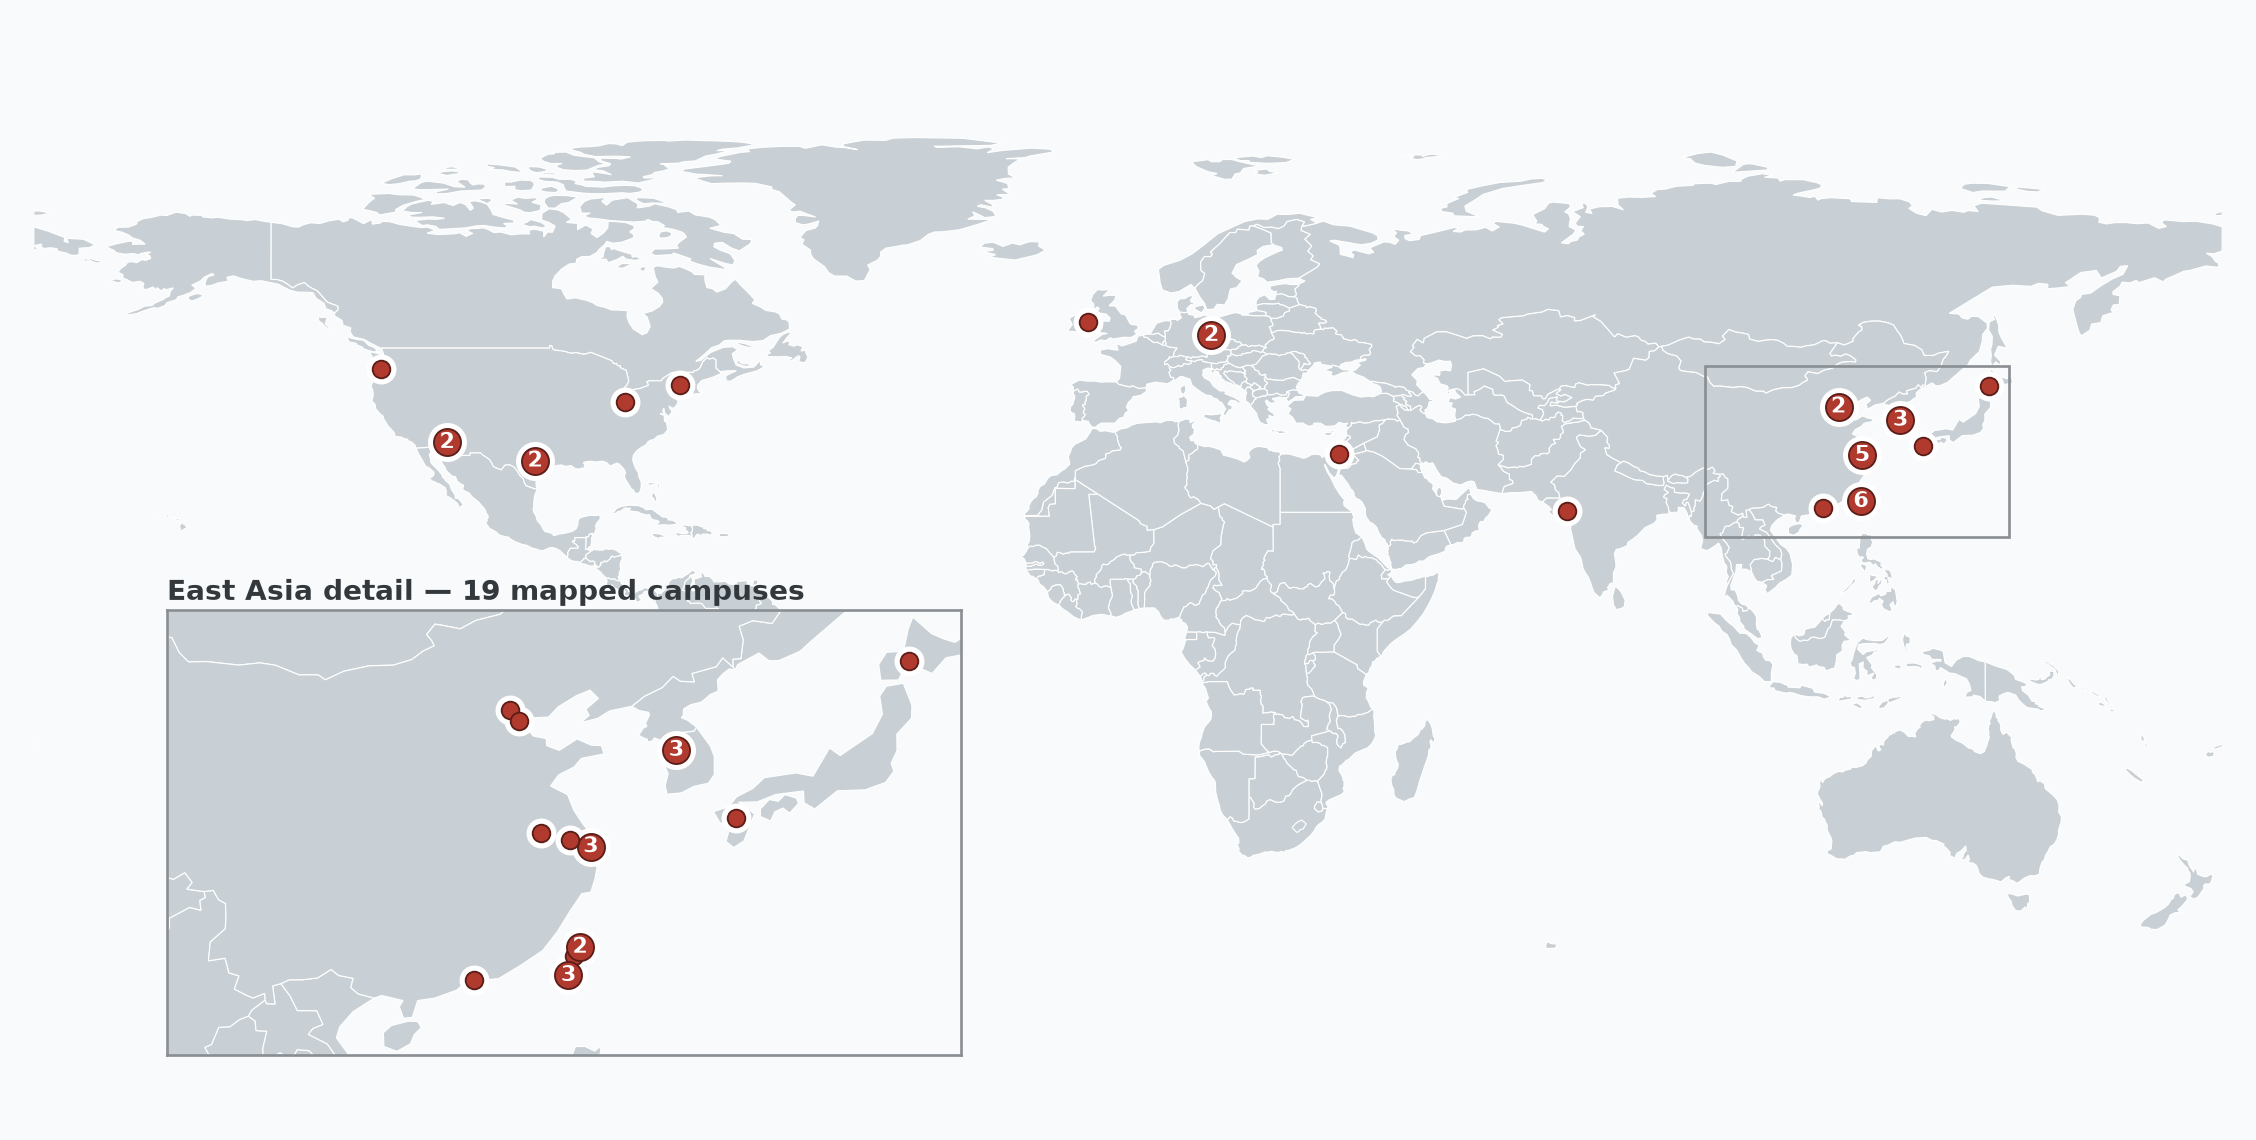
\includegraphics[width=\linewidth,keepaspectratio]{../figures/campus-locators/all-located-fabs-world-map.png}
\vfill
{\sffamily\scriptsize\color{black!58} Evidence reviewed through August 25, 2026.\par}
\end{minipage}
\clearpage
% Campus profile AIFAB-025
\markright{Fab 12B}
\noindent\begin{minipage}[t][0.90\textheight][t]{\textwidth}
\noindent\begin{minipage}[t]{0.69\textwidth}
\raggedright
{\sffamily\bfseries\Large\color{accent} Fab 12B\par}
\smallskip
{\sffamily\small\textbf{Operator:} TSMC\quad \textbf{Location:} Baoshan Township, Hsinchu County, TWN\par}
{\sffamily\footnotesize\color{black!68}\textbf{Facility status:} Operating (as of 2026-08-25)\par}
\end{minipage}
\hfill
\begin{minipage}[t]{0.27\textwidth}
\raggedright
{\sffamily\bfseries\footnotesize World location}\par\smallskip
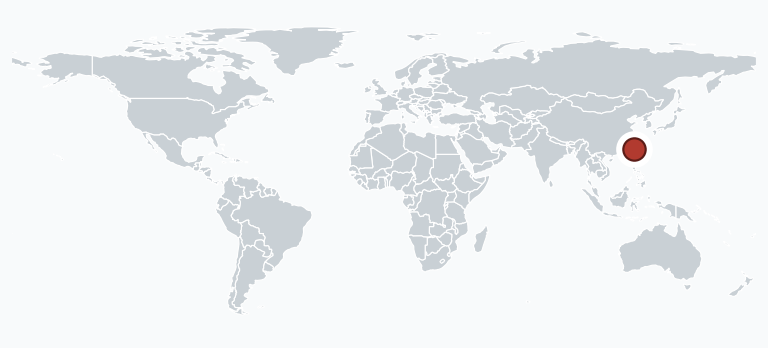
\includegraphics[width=\linewidth,keepaspectratio]{../figures/campus-locators/aifab-025-world-locator.png}
\par\smallskip
{\sffamily\scriptsize Coordinates: 24.770, 121.013.\par}
{\sffamily\scriptsize\color{black!68} Coordinates are the representative point returned for the cited OpenStreetMap feature.\nobreak\textsuperscript{\href{\detokenize{https://www.openstreetmap.org/way/717426548}}{\textcolor{accent}{1}}}\par}
\end{minipage}
\par\vspace{0.9em}
\noindent
\begin{minipage}[t]{\textwidth}
\raggedright
% Image-left evidence-right profile row
\begin{minipage}[t]{0.64\textwidth}
\vspace{0pt}\raggedright
\includegraphics[width=\linewidth,height=0.42\textheight,keepaspectratio,trim=0 0bp 0 0bp,clip]{../assets/campus-imagery/aifab-025.png}
\end{minipage}
\hfill
\begin{minipage}[t]{0.32\textwidth}
\vspace{0pt}\vspace{1.0em}\raggedright
{\sffamily\scriptsize Source: Taiwan Ministry of the Interior, National Land Surveying and Mapping Center, PHOTO2 orthophoto service; accessed August 6, 2026; acquisition date not stated; source extract 0.976562 m grid; 4 km view.\nobreak\textsuperscript{\href{\detokenize{https://maps.nlsc.gov.tw/S09SOA/pro/Wms_ajax_list.jsp}}{\textcolor{accent}{6}}} Yellow cross: cited location point.\par}
\medskip
{\footnotesize TSMC identifies Fab 12B as an operating 300 mm manufacturing site.\nobreak\textsuperscript{\href{\detokenize{https://www.openstreetmap.org/way/717426548}}{\textcolor{accent}{1}},\href{\detokenize{https://www.tsmc.com/english/aboutTSMC/TSMC_Fabs}}{\textcolor{accent}{2}},\href{\detokenize{https://investor.tsmc.com/sites/ir/annual-report/2024/2024}\%\detokenize{20Annual}\%\detokenize{20Report-E.pdf}}{\textcolor{accent}{3}},\href{\detokenize{https://web.archive.org/web/20260822170034/https://www.tsmc.com/english/aboutTSMC/executives.htm}}{\textcolor{accent}{4}},\href{\detokenize{https://investor.tsmc.com/sites/ir/sec-filings/2025_20F}\%\detokenize{20Report.pdf}}{\textcolor{accent}{5}}}\par}
\medskip
{\footnotesize\textbf{Documented wafer-fabrication capability:} Operating 300 mm manufacturing; 40 nm was the most advanced volume-production technology reported for Fab 12 at year-end 2025\nobreak\textsuperscript{\href{\detokenize{https://web.archive.org/web/20260822170034/https://www.tsmc.com/english/aboutTSMC/executives.htm}}{\textcolor{accent}{4}},\href{\detokenize{https://investor.tsmc.com/sites/ir/sec-filings/2025_20F}\%\detokenize{20Report.pdf}}{\textcolor{accent}{5}}}\par}
\end{minipage}
\end{minipage}
\par\vspace{0.65em}
\medskip
{\footnotesize\textbf{Named data-center AI accelerators or programs:} None identified in the sources reviewed.\par}
\smallskip
{\sffamily\scriptsize\color{black!62}\textbf{Other public catalogues (same campus; reviewed August 25, 2026):} \href{\detokenize{https://en.wikipedia.org/w/index.php?title=List_of_semiconductor_fabrication_plants&oldid=1370451124}\#\detokenize{Open_plants}}{Wikipedia fab list}.\par}
\medskip
{\sffamily\scriptsize\setlength{\emergencystretch}{1.5em}\textbf{Sources.} \textsuperscript{1}\,OpenStreetMap contributors. \href{\detokenize{https://www.openstreetmap.org/way/717426548}}{\enquote{TSMC Fab 12 mapped industrial area, OSM way 717426548.}} Accessed August 25, 2026; \textsuperscript{2}\,TSMC. \href{\detokenize{https://www.tsmc.com/english/aboutTSMC/TSMC_Fabs}}{\enquote{TSMC global manufacturing facilities.}} Accessed August 11, 2026; \textsuperscript{3}\,TSMC. \href{\detokenize{https://investor.tsmc.com/sites/ir/annual-report/2024/2024}\%\detokenize{20Annual}\%\detokenize{20Report-E.pdf}}{\enquote{TSMC 2024 Annual Report.}} March 12, 2025; \textsuperscript{4}\,TSMC. \href{\detokenize{https://web.archive.org/web/20260822170034/https://www.tsmc.com/english/aboutTSMC/executives.htm}}{\enquote{TSMC executive profiles describing site-specific process histories.}} Archived August 22, 2026; \textsuperscript{5}\,TSMC. \href{\detokenize{https://investor.tsmc.com/sites/ir/sec-filings/2025_20F}\%\detokenize{20Report.pdf}}{\enquote{2025 Form 20-F.}} April 16, 2026; \textsuperscript{6}\,Taiwan Ministry of the Interior, National Land Surveying and Mapping Center. \href{\detokenize{https://maps.nlsc.gov.tw/S09SOA/pro/Wms_ajax_list.jsp}}{\enquote{PHOTO2 general orthophoto service.}} Accessed August 6, 2026.\par}
\vfill
\noindent{\color{hairline}\rule{\linewidth}{0.4pt}}\par\smallskip
{\sffamily\scriptsize\color{black!58} Evidence reviewed through August 25, 2026.\par}
\end{minipage}
\clearpage
% Campus profile AIFAB-010
\markright{Fab 14B}
\noindent\begin{minipage}[t][0.90\textheight][t]{\textwidth}
\noindent\begin{minipage}[t]{0.69\textwidth}
\raggedright
{\sffamily\bfseries\Large\color{accent} Fab 14B\par}
\smallskip
{\sffamily\small\textbf{Operator:} TSMC\quad \textbf{Location:} Shanhua District, Tainan City, TWN\par}
{\sffamily\footnotesize\color{black!68}\textbf{Facility status:} Operating (as of 2026-08-25)\par}
\end{minipage}
\hfill
\begin{minipage}[t]{0.27\textwidth}
\raggedright
{\sffamily\bfseries\footnotesize World location}\par\smallskip
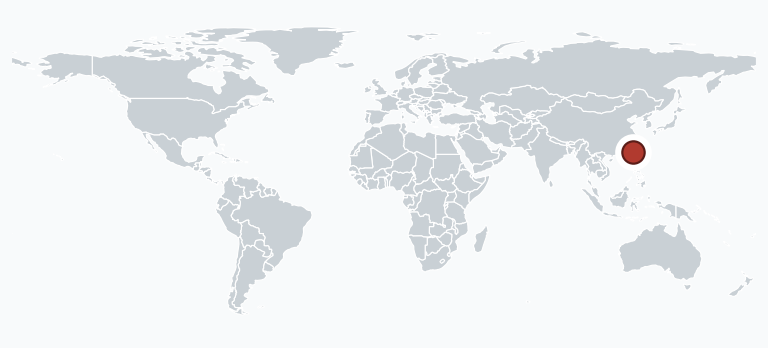
\includegraphics[width=\linewidth,keepaspectratio]{../figures/campus-locators/aifab-010-world-locator.png}
\par\smallskip
{\sffamily\scriptsize Coordinates: 23.111, 120.268.\par}
{\sffamily\scriptsize\color{black!68} Coordinates are the representative point returned for the cited OpenStreetMap feature.\nobreak\textsuperscript{\href{\detokenize{https://www.openstreetmap.org/way/1369955775}}{\textcolor{accent}{1}}}\par}
\end{minipage}
\par\vspace{0.9em}
\noindent
\begin{minipage}[t]{\textwidth}
\raggedright
% Image-left evidence-right profile row
\begin{minipage}[t]{0.64\textwidth}
\vspace{0pt}\raggedright
\includegraphics[width=\linewidth,height=0.42\textheight,keepaspectratio,trim=0 0bp 0 0bp,clip]{../assets/campus-imagery/aifab-010.png}
\end{minipage}
\hfill
\begin{minipage}[t]{0.32\textwidth}
\vspace{0pt}\vspace{1.0em}\raggedright
{\sffamily\scriptsize Source: Taiwan Ministry of the Interior, National Land Surveying and Mapping Center, PHOTO2 orthophoto service; accessed August 23, 2026; acquisition date not stated; source extract 0.976562 m grid; 4 km view.\nobreak\textsuperscript{\href{\detokenize{https://maps.nlsc.gov.tw/S09SOA/pro/Wms_ajax_list.jsp}}{\textcolor{accent}{5}}} Yellow cross: cited location point.\par}
\medskip
{\footnotesize TSMC identifies Fab 14B as a distinct manufacturing site and documented 12/16 nm wafer production there.\nobreak\textsuperscript{\href{\detokenize{https://www.tsmc.com/english/aboutTSMC/TSMC_Fabs}}{\textcolor{accent}{2}},\href{\detokenize{https://investor.tsmc.com/sites/ir/sec-filings/2025_20F}\%\detokenize{20Report.pdf}}{\textcolor{accent}{3}},\href{\detokenize{https://pr.tsmc.com/english/news/1984}}{\textcolor{accent}{4}}}\par}
\medskip
{\footnotesize\textbf{Documented wafer-fabrication capability:} TSMC documented 12/16 nm wafer production at Fab 14B in 2019; the current product mix is not disclosed.\nobreak\textsuperscript{\href{\detokenize{https://pr.tsmc.com/english/news/1984}}{\textcolor{accent}{4}}}\par}
\end{minipage}
\end{minipage}
\par\vspace{0.65em}
\medskip
{\footnotesize\textbf{Named data-center AI accelerators or programs:} None identified in the sources reviewed.\par}
\smallskip
{\sffamily\scriptsize\color{black!62}\textbf{Other public catalogues (same campus; reviewed August 25, 2026):} \href{\detokenize{https://en.wikipedia.org/w/index.php?title=List_of_semiconductor_fabrication_plants&oldid=1370451124}\#\detokenize{Open_plants}}{Wikipedia fab list}.\par}
\medskip
{\sffamily\scriptsize\setlength{\emergencystretch}{1.5em}\textbf{Sources.} \textsuperscript{1}\,OpenStreetMap contributors. \href{\detokenize{https://www.openstreetmap.org/way/1369955775}}{\enquote{TSMC Fab 14 Phase 6 mapped building, OSM way 1369955775.}} Accessed August 11, 2026; \textsuperscript{2}\,TSMC. \href{\detokenize{https://www.tsmc.com/english/aboutTSMC/TSMC_Fabs}}{\enquote{TSMC global manufacturing facilities.}} Accessed August 11, 2026; \textsuperscript{3}\,TSMC. \href{\detokenize{https://investor.tsmc.com/sites/ir/sec-filings/2025_20F}\%\detokenize{20Report.pdf}}{\enquote{2025 Form 20-F.}} April 16, 2026; \textsuperscript{4}\,TSMC. \href{\detokenize{https://pr.tsmc.com/english/news/1984}}{\enquote{TSMC Details Impact of Fab 14B Photoresist Material Incident, Updates 1Q'19 Guidance.}} February 15, 2019; \textsuperscript{5}\,Taiwan Ministry of the Interior, National Land Surveying and Mapping Center. \href{\detokenize{https://maps.nlsc.gov.tw/S09SOA/pro/Wms_ajax_list.jsp}}{\enquote{PHOTO2 general orthophoto service.}} Accessed August 23, 2026.\par}
\vfill
\noindent{\color{hairline}\rule{\linewidth}{0.4pt}}\par\smallskip
{\sffamily\scriptsize\color{black!58} Evidence reviewed through August 25, 2026.\par}
\end{minipage}
\clearpage
% Campus profile AIFAB-001
\markright{Fab 15B}
\noindent\begin{minipage}[t][0.90\textheight][t]{\textwidth}
\noindent\begin{minipage}[t]{0.69\textwidth}
\raggedright
{\sffamily\bfseries\Large\color{accent} Fab 15B\par}
\smallskip
{\sffamily\small\textbf{Operator:} TSMC\quad \textbf{Location:} Xitun District, Taichung City, TWN\par}
{\sffamily\footnotesize\color{black!68}\textbf{Facility status:} Operating (as of 2026-08-25)\par}
\end{minipage}
\hfill
\begin{minipage}[t]{0.27\textwidth}
\raggedright
{\sffamily\bfseries\footnotesize World location}\par\smallskip
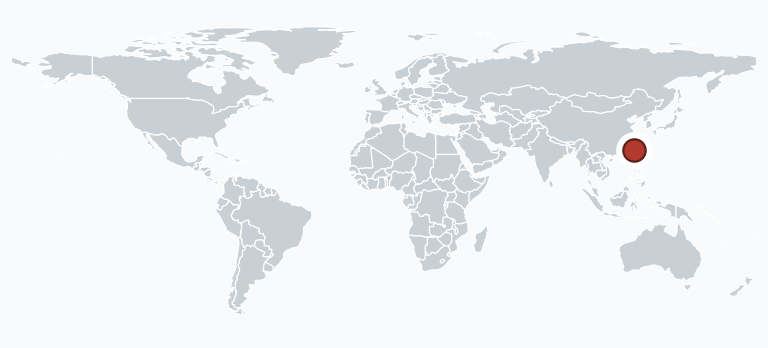
\includegraphics[width=\linewidth,keepaspectratio]{../figures/campus-locators/aifab-001-world-locator.png}
\par\smallskip
{\sffamily\scriptsize Coordinates: 24.212, 120.609.\par}
{\sffamily\scriptsize\color{black!68} Coordinates from TSMC's cited facilities listing.\nobreak\textsuperscript{\href{\detokenize{https://maps.app.goo.gl/ctdzf84Wjd5HqFJ28}}{\textcolor{accent}{1}}}\par}
\end{minipage}
\par\vspace{0.9em}
\noindent
\begin{minipage}[t]{\textwidth}
\raggedright
% Image-left evidence-right profile row
\begin{minipage}[t]{0.64\textwidth}
\vspace{0pt}\raggedright
\includegraphics[width=\linewidth,height=0.42\textheight,keepaspectratio,trim=0 0bp 0 0bp,clip]{../assets/campus-imagery/aifab-001.png}
\end{minipage}
\hfill
\begin{minipage}[t]{0.32\textwidth}
\vspace{0pt}\vspace{1.0em}\raggedright
{\sffamily\scriptsize Source: Taiwan Ministry of the Interior, National Land Surveying and Mapping Center, PHOTO2 orthophoto service; accessed August 6, 2026; acquisition date not stated; source extract 0.976562 m grid; 4 km view.\nobreak\textsuperscript{\href{\detokenize{https://maps.nlsc.gov.tw/S09SOA/pro/Wms_ajax_list.jsp}}{\textcolor{accent}{5}}} Yellow cross: cited location point.\par}
\medskip
{\footnotesize TSMC identifies Fab 15B as an operating manufacturing campus.\nobreak\textsuperscript{\href{\detokenize{https://maps.app.goo.gl/ctdzf84Wjd5HqFJ28}}{\textcolor{accent}{1}},\href{\detokenize{https://www.tsmc.com/english/aboutTSMC/TSMC_Fabs}}{\textcolor{accent}{2}},\href{\detokenize{https://investor.tsmc.com/sites/ir/sec-filings/2025_20F}\%\detokenize{20Report.pdf}}{\textcolor{accent}{3}},\href{\detokenize{https://web.archive.org/web/20260822170034/https://www.tsmc.com/english/aboutTSMC/executives.htm}}{\textcolor{accent}{4}}}\par}
\medskip
{\footnotesize\textbf{Documented wafer-fabrication capability:} TSMC states that Fab 15B began with 10 nm technology in 2017 and migrated to 7 nm in 2018; current product allocation is not disclosed.\nobreak\textsuperscript{\href{\detokenize{https://web.archive.org/web/20260822170034/https://www.tsmc.com/english/aboutTSMC/executives.htm}}{\textcolor{accent}{4}}}\par}
\end{minipage}
\end{minipage}
\par\vspace{0.65em}
\medskip
{\footnotesize\textbf{Named data-center AI accelerators or programs:} None identified in the sources reviewed.\par}
\smallskip
{\sffamily\scriptsize\color{black!62}\textbf{Other public catalogues (same campus; reviewed August 25, 2026):} \href{\detokenize{https://en.wikipedia.org/w/index.php?title=List_of_semiconductor_fabrication_plants&oldid=1370451124}\#\detokenize{Open_plants}}{Wikipedia fab list}.\par}
\medskip
{\sffamily\scriptsize\setlength{\emergencystretch}{1.5em}\textbf{Sources.} \textsuperscript{1}\,TSMC. \href{\detokenize{https://maps.app.goo.gl/ctdzf84Wjd5HqFJ28}}{\enquote{Operator-linked map point for TSMC Fab 15B.}} Accessed August 25, 2026; \textsuperscript{2}\,TSMC. \href{\detokenize{https://www.tsmc.com/english/aboutTSMC/TSMC_Fabs}}{\enquote{TSMC global manufacturing facilities.}} Accessed August 11, 2026; \textsuperscript{3}\,TSMC. \href{\detokenize{https://investor.tsmc.com/sites/ir/sec-filings/2025_20F}\%\detokenize{20Report.pdf}}{\enquote{2025 Form 20-F.}} April 16, 2026; \textsuperscript{4}\,TSMC. \href{\detokenize{https://web.archive.org/web/20260822170034/https://www.tsmc.com/english/aboutTSMC/executives.htm}}{\enquote{TSMC executive profiles describing site-specific process histories.}} Archived August 22, 2026; \textsuperscript{5}\,Taiwan Ministry of the Interior, National Land Surveying and Mapping Center. \href{\detokenize{https://maps.nlsc.gov.tw/S09SOA/pro/Wms_ajax_list.jsp}}{\enquote{PHOTO2 general orthophoto service.}} Accessed August 6, 2026.\par}
\vfill
\noindent{\color{hairline}\rule{\linewidth}{0.4pt}}\par\smallskip
{\sffamily\scriptsize\color{black!58} Evidence reviewed through August 25, 2026.\par}
\end{minipage}
\clearpage
% Campus profile AIFAB-002
\markright{Fab 18A/B}
\noindent\begin{minipage}[t][0.90\textheight][t]{\textwidth}
\noindent\begin{minipage}[t]{0.69\textwidth}
\raggedright
{\sffamily\bfseries\Large\color{accent} Fab 18A/B\par}
\smallskip
{\sffamily\small\textbf{Operator:} TSMC\quad \textbf{Location:} Tainan, TWN\par}
{\sffamily\footnotesize\color{black!68}\textbf{Facility status:} Operating (as of 2026-08-10)\par}
\end{minipage}
\hfill
\begin{minipage}[t]{0.27\textwidth}
\raggedright
{\sffamily\bfseries\footnotesize World location}\par\smallskip
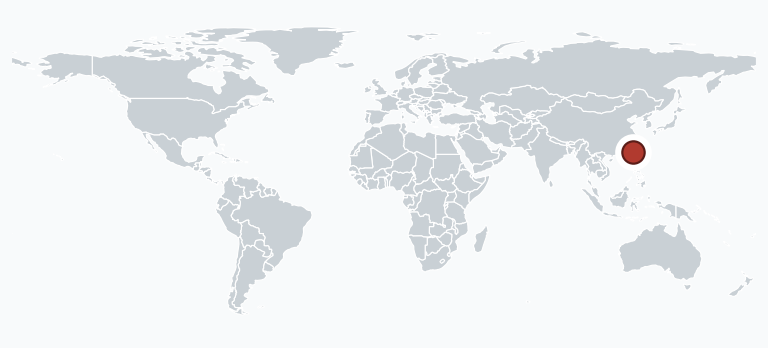
\includegraphics[width=\linewidth,keepaspectratio]{../figures/campus-locators/aifab-002-world-locator.png}
\par\smallskip
{\sffamily\scriptsize Coordinates: 23.116, 120.264.\par}
{\sffamily\scriptsize\color{black!68} Coordinates from TSMC's cited facilities listing.\nobreak\textsuperscript{\href{\detokenize{https://www.tsmc.com/english/aboutTSMC/TSMC_Fabs}}{\textcolor{accent}{1}}}\par}
\end{minipage}
\par\vspace{0.9em}
\noindent
\begin{minipage}[t]{\textwidth}
\raggedright
% Image-left evidence-right profile row
\begin{minipage}[t]{0.64\textwidth}
\vspace{0pt}\raggedright
\includegraphics[width=\linewidth,height=0.42\textheight,keepaspectratio,trim=0 0bp 0 0bp,clip]{../assets/campus-imagery/aifab-002.png}
\end{minipage}
\hfill
\begin{minipage}[t]{0.32\textwidth}
\vspace{0pt}\vspace{1.0em}\raggedright
{\sffamily\scriptsize Source: Taiwan Ministry of the Interior, National Land Surveying and Mapping Center, PHOTO2 orthophoto service; accessed August 6, 2026; acquisition date not stated; source extract 0.976562 m grid; 4 km view.\nobreak\textsuperscript{\href{\detokenize{https://maps.nlsc.gov.tw/S09SOA/pro/Wms_ajax_list.jsp}}{\textcolor{accent}{4}}} Yellow cross: cited location point.\par}
\medskip
{\footnotesize TSMC identifies Fab 18 and its history of N5, N4, and N3 production. These processes are suitable for advanced AI chips.\nobreak\textsuperscript{\href{\detokenize{https://www.tsmc.com/english/aboutTSMC/TSMC_Fabs}}{\textcolor{accent}{1}},\href{\detokenize{https://pr.tsmc.com/english/news/2986}}{\textcolor{accent}{2}},\href{\detokenize{https://web.archive.org/web/20260822170034/https://www.tsmc.com/english/aboutTSMC/executives.htm}}{\textcolor{accent}{3}}}\par}
\medskip
{\footnotesize\textbf{Documented wafer-fabrication capability:} N5/N4/N3\nobreak\textsuperscript{\href{\detokenize{https://pr.tsmc.com/english/news/2986}}{\textcolor{accent}{2}},\href{\detokenize{https://web.archive.org/web/20260822170034/https://www.tsmc.com/english/aboutTSMC/executives.htm}}{\textcolor{accent}{3}}}\par}
\end{minipage}
\end{minipage}
\par\vspace{0.65em}
\medskip
{\footnotesize\textbf{Named data-center AI accelerators or programs:} None identified in the sources reviewed.\par}
\smallskip
{\sffamily\scriptsize\color{black!62}\textbf{Other public catalogues (same campus; reviewed August 25, 2026):} \href{\detokenize{https://en.wikipedia.org/w/index.php?title=List_of_semiconductor_fabrication_plants&oldid=1370451124}\#\detokenize{Open_plants}}{Wikipedia fab list}.\par}
\medskip
{\sffamily\scriptsize\setlength{\emergencystretch}{1.5em}\textbf{Sources.} \textsuperscript{1}\,TSMC. \href{\detokenize{https://www.tsmc.com/english/aboutTSMC/TSMC_Fabs}}{\enquote{TSMC global manufacturing facilities.}} Accessed August 11, 2026; \textsuperscript{2}\,TSMC. \href{\detokenize{https://pr.tsmc.com/english/news/2986}}{\enquote{TSMC Holds 3nm Volume Production and Capacity Expansion Ceremony, Marking a Key Milestone for Advanced Manufacturing.}} December 29, 2022; \textsuperscript{3}\,TSMC. \href{\detokenize{https://web.archive.org/web/20260822170034/https://www.tsmc.com/english/aboutTSMC/executives.htm}}{\enquote{TSMC executive profiles describing site-specific process histories.}} Archived August 22, 2026; \textsuperscript{4}\,Taiwan Ministry of the Interior, National Land Surveying and Mapping Center. \href{\detokenize{https://maps.nlsc.gov.tw/S09SOA/pro/Wms_ajax_list.jsp}}{\enquote{PHOTO2 general orthophoto service.}} Accessed August 6, 2026.\par}
\vfill
\noindent{\color{hairline}\rule{\linewidth}{0.4pt}}\par\smallskip
{\sffamily\scriptsize\color{black!58} Evidence reviewed through August 25, 2026.\par}
\end{minipage}
\clearpage
% Campus profile AIFAB-004
\markright{Fab 20}
\noindent\begin{minipage}[t][0.90\textheight][t]{\textwidth}
\noindent\begin{minipage}[t]{0.69\textwidth}
\raggedright
{\sffamily\bfseries\Large\color{accent} Fab 20\par}
\smallskip
{\sffamily\small\textbf{Operator:} TSMC\quad \textbf{Location:} Baoshan Township (Hsinchu Science Park), Hsinchu County, TWN\par}
{\sffamily\footnotesize\color{black!68}\textbf{Facility status:} Operating; production ramp and phased expansion continuing (as of 2026-08-25)\par}
\end{minipage}
\hfill
\begin{minipage}[t]{0.27\textwidth}
\raggedright
{\sffamily\bfseries\footnotesize World location}\par\smallskip
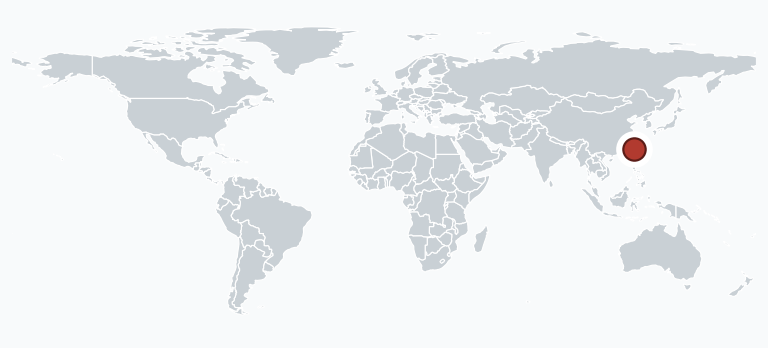
\includegraphics[width=\linewidth,keepaspectratio]{../figures/campus-locators/aifab-004-world-locator.png}
\par\smallskip
{\sffamily\scriptsize Coordinates: 24.766, 121.002.\par}
{\sffamily\scriptsize\color{black!68} Coordinates derived from the cited science-park project record.\nobreak\textsuperscript{\href{\detokenize{https://pavo.sipa.gov.tw/sppc/bleppage02.html}}{\textcolor{accent}{1}}}\par}
\end{minipage}
\par\vspace{0.9em}
\noindent
\begin{minipage}[t]{\textwidth}
\raggedright
% Image-left evidence-right profile row
\begin{minipage}[t]{0.64\textwidth}
\vspace{0pt}\raggedright
\includegraphics[width=\linewidth,height=0.42\textheight,keepaspectratio,trim=0 0bp 0 0bp,clip]{../assets/campus-imagery/aifab-004.png}
\end{minipage}
\hfill
\begin{minipage}[t]{0.32\textwidth}
\vspace{0pt}\vspace{1.0em}\raggedright
{\sffamily\scriptsize Source: Taiwan Ministry of the Interior, National Land Surveying and Mapping Center, PHOTO2 orthophoto service; accessed August 6, 2026; acquisition date not stated; source extract 0.976562 m grid; 4 km view.\nobreak\textsuperscript{\href{\detokenize{https://maps.nlsc.gov.tw/S09SOA/pro/Wms_ajax_list.jsp}}{\textcolor{accent}{6}}} Yellow cross: cited location point.\par}
\medskip
{\footnotesize TSMC identifies Fab 20 as an operating N2 campus whose commercial production began in 2025. TSMC also describes a multi-phase ramp and expansion at Hsinchu supported by smartphone, high-performance-computing, and AI demand.\nobreak\textsuperscript{\href{\detokenize{https://www.tsmc.com/english/aboutTSMC/TSMC_Fabs}}{\textcolor{accent}{2}},\href{\detokenize{https://investor.tsmc.com/sites/ir/sec-filings/2025_20F}\%\detokenize{20Report.pdf}}{\textcolor{accent}{3}},\href{\detokenize{https://www.tsmc.com/english/dedicatedFoundry/technology/logic/l_2nm}}{\textcolor{accent}{4}},\href{\detokenize{https://investor.tsmc.com/chinese/encrypt/files/encrypt_file/reports/2026-04/3cef85204275f94fd111485cfdf4adb3c0263c45/TSMC}\%\detokenize{201Q26}\%\detokenize{20Transcript.pdf}}{\textcolor{accent}{5}}}\par}
\medskip
{\footnotesize\textbf{Documented wafer-fabrication capability:} Operating 12-inch fab; N2 is its most advanced volume-production technology; multi-phase ramp and expansion continue\nobreak\textsuperscript{\href{\detokenize{https://investor.tsmc.com/sites/ir/sec-filings/2025_20F}\%\detokenize{20Report.pdf}}{\textcolor{accent}{3}},\href{\detokenize{https://www.tsmc.com/english/dedicatedFoundry/technology/logic/l_2nm}}{\textcolor{accent}{4}},\href{\detokenize{https://investor.tsmc.com/chinese/encrypt/files/encrypt_file/reports/2026-04/3cef85204275f94fd111485cfdf4adb3c0263c45/TSMC}\%\detokenize{201Q26}\%\detokenize{20Transcript.pdf}}{\textcolor{accent}{5}}}\par}
\end{minipage}
\end{minipage}
\par\vspace{0.65em}
\medskip
{\footnotesize\textbf{Named data-center AI accelerators or programs:} None identified in the sources reviewed.\par}
\medskip
{\sffamily\scriptsize\setlength{\emergencystretch}{1.5em}\textbf{Sources.} \textsuperscript{1}\,Hsinchu Science Park Bureau. \href{\detokenize{https://pavo.sipa.gov.tw/sppc/bleppage02.html}}{\enquote{Baoshan Phase 2 expansion project: second tender.}} Accessed August 11, 2026; \textsuperscript{2}\,TSMC. \href{\detokenize{https://www.tsmc.com/english/aboutTSMC/TSMC_Fabs}}{\enquote{TSMC global manufacturing facilities.}} Accessed August 11, 2026; \textsuperscript{3}\,TSMC. \href{\detokenize{https://investor.tsmc.com/sites/ir/sec-filings/2025_20F}\%\detokenize{20Report.pdf}}{\enquote{2025 Form 20-F.}} April 16, 2026; \textsuperscript{4}\,TSMC. \href{\detokenize{https://www.tsmc.com/english/dedicatedFoundry/technology/logic/l_2nm}}{\enquote{TSMC N2 logic technology.}} Accessed August 11, 2026; \textsuperscript{5}\,TSMC. \href{\detokenize{https://investor.tsmc.com/chinese/encrypt/files/encrypt_file/reports/2026-04/3cef85204275f94fd111485cfdf4adb3c0263c45/TSMC}\%\detokenize{201Q26}\%\detokenize{20Transcript.pdf}}{\enquote{First Quarter 2026 Earnings Conference Transcript.}} April 16, 2026; \textsuperscript{6}\,Taiwan Ministry of the Interior, National Land Surveying and Mapping Center. \href{\detokenize{https://maps.nlsc.gov.tw/S09SOA/pro/Wms_ajax_list.jsp}}{\enquote{PHOTO2 general orthophoto service.}} Accessed August 6, 2026.\par}
\vfill
\noindent{\color{hairline}\rule{\linewidth}{0.4pt}}\par\smallskip
{\sffamily\scriptsize\color{black!58} Evidence reviewed through August 25, 2026.\par}
\end{minipage}
\clearpage
% Campus profile AIFAB-005
\markright{Fab 22}
\noindent\begin{minipage}[t][0.90\textheight][t]{\textwidth}
\noindent\begin{minipage}[t]{0.69\textwidth}
\raggedright
{\sffamily\bfseries\Large\color{accent} Fab 22\par}
\smallskip
{\sffamily\small\textbf{Operator:} TSMC\quad \textbf{Location:} Kaohsiung, TWN\par}
{\sffamily\footnotesize\color{black!68}\textbf{Facility status:} Operating; production ramp and phased expansion continuing (as of 2026-08-25)\par}
\end{minipage}
\hfill
\begin{minipage}[t]{0.27\textwidth}
\raggedright
{\sffamily\bfseries\footnotesize World location}\par\smallskip
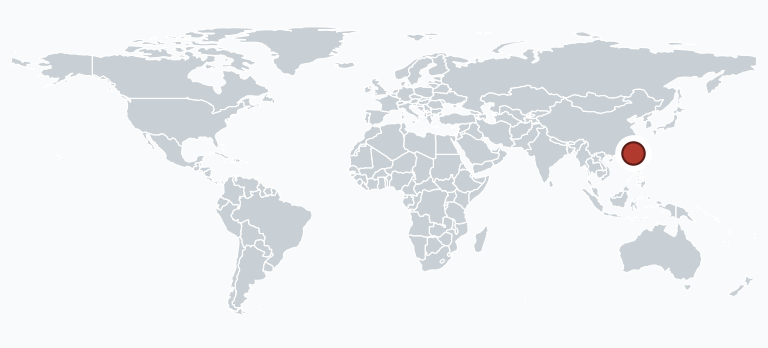
\includegraphics[width=\linewidth,keepaspectratio]{../figures/campus-locators/aifab-005-world-locator.png}
\par\smallskip
{\sffamily\scriptsize Coordinates: 22.713, 120.309.\par}
{\sffamily\scriptsize\color{black!68} Coordinates from the official site/event point in the cited government record.\nobreak\textsuperscript{\href{\detokenize{https://www.ey.gov.tw/Page/278197D37F0FCDA?ED=20250331&K=&SD=20250331&T=1&page=1}}{\textcolor{accent}{1}}}\par}
\end{minipage}
\par\vspace{0.9em}
\noindent
\begin{minipage}[t]{\textwidth}
\raggedright
% Image-left evidence-right profile row
\begin{minipage}[t]{0.64\textwidth}
\vspace{0pt}\raggedright
\includegraphics[width=\linewidth,height=0.42\textheight,keepaspectratio,trim=0 0bp 0 0bp,clip]{../assets/campus-imagery/aifab-005.png}
\end{minipage}
\hfill
\begin{minipage}[t]{0.32\textwidth}
\vspace{0pt}\vspace{1.0em}\raggedright
{\sffamily\scriptsize Source: Taiwan Ministry of the Interior, National Land Surveying and Mapping Center, PHOTO2 orthophoto service; accessed August 6, 2026; acquisition date not stated; source extract 0.976562 m grid; 4 km view.\nobreak\textsuperscript{\href{\detokenize{https://maps.nlsc.gov.tw/S09SOA/pro/Wms_ajax_list.jsp}}{\textcolor{accent}{7}}} Yellow cross: cited location point.\par}
\medskip
{\footnotesize TSMC identifies Fab 22 as an operating N2 campus whose commercial production began in 2025. Official sources support Phases 1--5 planned and a multi-phase production ramp, with expansion continuing.\nobreak\textsuperscript{\href{\detokenize{https://www.tsmc.com/english/aboutTSMC/TSMC_Fabs}}{\textcolor{accent}{2}},\href{\detokenize{https://investor.tsmc.com/sites/ir/sec-filings/2025_20F}\%\detokenize{20Report.pdf}}{\textcolor{accent}{3}},\href{\detokenize{https://www.stsp.gov.tw/attached/Letter/Ebook/316/files/basic-html/page5.html}}{\textcolor{accent}{4}},\href{\detokenize{https://www.tsmc.com/english/dedicatedFoundry/technology/logic/l_2nm}}{\textcolor{accent}{5}},\href{\detokenize{https://investor.tsmc.com/chinese/encrypt/files/encrypt_file/reports/2026-04/3cef85204275f94fd111485cfdf4adb3c0263c45/TSMC}\%\detokenize{201Q26}\%\detokenize{20Transcript.pdf}}{\textcolor{accent}{6}}}\par}
\medskip
{\footnotesize\textbf{Documented wafer-fabrication capability:} Operating 12-inch fab; N2 is its most advanced volume-production technology; Phases 1--5 are planned and a multi-phase production ramp is under way\nobreak\textsuperscript{\href{\detokenize{https://investor.tsmc.com/sites/ir/sec-filings/2025_20F}\%\detokenize{20Report.pdf}}{\textcolor{accent}{3}},\href{\detokenize{https://www.stsp.gov.tw/attached/Letter/Ebook/316/files/basic-html/page5.html}}{\textcolor{accent}{4}},\href{\detokenize{https://www.tsmc.com/english/dedicatedFoundry/technology/logic/l_2nm}}{\textcolor{accent}{5}},\href{\detokenize{https://investor.tsmc.com/chinese/encrypt/files/encrypt_file/reports/2026-04/3cef85204275f94fd111485cfdf4adb3c0263c45/TSMC}\%\detokenize{201Q26}\%\detokenize{20Transcript.pdf}}{\textcolor{accent}{6}}}\par}
\end{minipage}
\end{minipage}
\par\vspace{0.65em}
\medskip
{\footnotesize\textbf{Named data-center AI accelerators or programs:} None identified in the sources reviewed.\par}
\medskip
{\sffamily\scriptsize\setlength{\emergencystretch}{1.5em}\textbf{Sources.} \textsuperscript{1}\,Executive Yuan, Republic of China (Taiwan). \href{\detokenize{https://www.ey.gov.tw/Page/278197D37F0FCDA?ED=20250331&K=&SD=20250331&T=1&page=1}}{\enquote{Premier's March 31, 2025 schedule: TSMC Fab 22 expansion ceremony.}} March 31, 2025; \textsuperscript{2}\,TSMC. \href{\detokenize{https://www.tsmc.com/english/aboutTSMC/TSMC_Fabs}}{\enquote{TSMC global manufacturing facilities.}} Accessed August 11, 2026; \textsuperscript{3}\,TSMC. \href{\detokenize{https://investor.tsmc.com/sites/ir/sec-filings/2025_20F}\%\detokenize{20Report.pdf}}{\enquote{2025 Form 20-F.}} April 16, 2026; \textsuperscript{4}\,Southern Taiwan Science Park Bureau. \href{\detokenize{https://www.stsp.gov.tw/attached/Letter/Ebook/316/files/basic-html/page5.html}}{\enquote{The Expansion of TSMC 2nm Production in the Nanzih Science Park.}} May 2025; \textsuperscript{5}\,TSMC. \href{\detokenize{https://www.tsmc.com/english/dedicatedFoundry/technology/logic/l_2nm}}{\enquote{TSMC N2 logic technology.}} Accessed August 11, 2026; \textsuperscript{6}\,TSMC. \href{\detokenize{https://investor.tsmc.com/chinese/encrypt/files/encrypt_file/reports/2026-04/3cef85204275f94fd111485cfdf4adb3c0263c45/TSMC}\%\detokenize{201Q26}\%\detokenize{20Transcript.pdf}}{\enquote{First Quarter 2026 Earnings Conference Transcript.}} April 16, 2026; \textsuperscript{7}\,Taiwan Ministry of the Interior, National Land Surveying and Mapping Center. \href{\detokenize{https://maps.nlsc.gov.tw/S09SOA/pro/Wms_ajax_list.jsp}}{\enquote{PHOTO2 general orthophoto service.}} Accessed August 6, 2026.\par}
\vfill
\noindent{\color{hairline}\rule{\linewidth}{0.4pt}}\par\smallskip
{\sffamily\scriptsize\color{black!58} Evidence reviewed through August 25, 2026.\par}
\end{minipage}
\clearpage
% Campus profile AIFAB-012
\markright{Giheung Campus}
\noindent\begin{minipage}[t][0.90\textheight][t]{\textwidth}
\noindent\begin{minipage}[t]{0.69\textwidth}
\raggedright
{\sffamily\bfseries\Large\color{accent} Giheung Campus\par}
\smallskip
{\sffamily\small\textbf{Operator:} Samsung Electronics\quad \textbf{Location:} Yongin, Gyeonggi-do, KOR\par}
{\sffamily\footnotesize\color{black!68}\textbf{Facility status:} Operating (as of 2026-08-10)\par}
\end{minipage}
\hfill
\begin{minipage}[t]{0.27\textwidth}
\raggedright
{\sffamily\bfseries\footnotesize World location}\par\smallskip
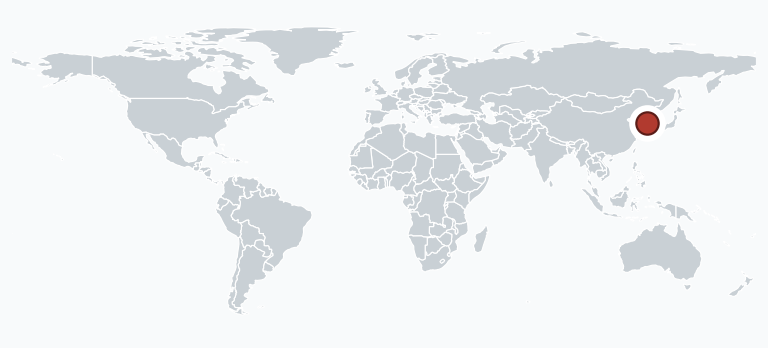
\includegraphics[width=\linewidth,keepaspectratio]{../figures/campus-locators/aifab-012-world-locator.png}
\par\smallskip
{\sffamily\scriptsize Coordinates: 37.229, 127.084.\par}
{\sffamily\scriptsize\color{black!68} Coordinates are the representative point returned for the cited OpenStreetMap feature.\nobreak\textsuperscript{\href{\detokenize{https://www.openstreetmap.org/way/326869111}}{\textcolor{accent}{1}}}\par}
\end{minipage}
\par\vspace{0.9em}
\noindent
\begin{minipage}[t]{\textwidth}
\raggedright
% Image-left evidence-right profile row
\begin{minipage}[t]{0.64\textwidth}
\vspace{0pt}\raggedright
\includegraphics[width=\linewidth,height=0.42\textheight,keepaspectratio,trim=0 0bp 0 0bp,clip]{../assets/campus-imagery/aifab-012.png}
\end{minipage}
\hfill
\begin{minipage}[t]{0.32\textwidth}
\vspace{0pt}\vspace{1.0em}\raggedright
{\sffamily\scriptsize World Imagery; source imagery dated December 22, 2025; source extract 0.537109 m grid; 2.2 km view. Source: Esri, Vantor, Earthstar Geographics, and the GIS User Community. Local imagery: Vantor Vivid Advanced (WV02), source dated 2025-12-22, Raster Basemaps 2026.R04. Map image is the intellectual property of Esri and is used herein under license. Copyright © 2026 Esri and its licensors. All rights reserved. Cropped and annotated by the authors.\nobreak\textsuperscript{\href{\detokenize{https://www.arcgis.com/home/item.html?id=10df2279f9684e4a9f6a7f08febac2a9}}{\textcolor{accent}{3}}} Yellow cross: cited location point.\par}
\medskip
{\footnotesize Samsung identifies Giheung as a manufacturing campus with processes through 8 nm.\nobreak\textsuperscript{\href{\detokenize{https://semiconductor.samsung.com/foundry/manufacturing/manufacturing-sites/}}{\textcolor{accent}{2}}}\par}
\medskip
{\footnotesize\textbf{Documented wafer-fabrication capability:} mainstream foundry through 8 nm\nobreak\textsuperscript{\href{\detokenize{https://semiconductor.samsung.com/foundry/manufacturing/manufacturing-sites/}}{\textcolor{accent}{2}}}\par}
\end{minipage}
\end{minipage}
\par\vspace{0.65em}
\medskip
{\footnotesize\textbf{Named data-center AI accelerators or programs:} None identified in the sources reviewed.\par}
\smallskip
{\sffamily\scriptsize\color{black!62}\textbf{Other public catalogues (same campus; reviewed August 25, 2026):} \href{\detokenize{https://en.wikipedia.org/w/index.php?title=List_of_semiconductor_fabrication_plants&oldid=1370451124}\#\detokenize{Open_plants}}{Wikipedia fab list}.\par}
\medskip
{\sffamily\scriptsize\setlength{\emergencystretch}{1.5em}\textbf{Sources.} \textsuperscript{1}\,OpenStreetMap contributors. \href{\detokenize{https://www.openstreetmap.org/way/326869111}}{\enquote{Samsung Electronics Giheung Campus mapped area, OSM way 326869111.}} Accessed August 11, 2026; \textsuperscript{2}\,Samsung Electronics. \href{\detokenize{https://semiconductor.samsung.com/foundry/manufacturing/manufacturing-sites/}}{\enquote{Samsung Foundry manufacturing sites.}} Accessed August 11, 2026; \textsuperscript{3}\,Esri. \href{\detokenize{https://www.arcgis.com/home/item.html?id=10df2279f9684e4a9f6a7f08febac2a9}}{\enquote{World Imagery.}} Accessed August 23, 2026.\par}
\vfill
\noindent{\color{hairline}\rule{\linewidth}{0.4pt}}\par\smallskip
{\sffamily\scriptsize\color{black!58} Evidence reviewed through August 25, 2026.\par}
\end{minipage}
\clearpage
% Campus profile AIFAB-008
\markright{Hwaseong Campus}
\noindent\begin{minipage}[t][0.90\textheight][t]{\textwidth}
\noindent\begin{minipage}[t]{0.69\textwidth}
\raggedright
{\sffamily\bfseries\Large\color{accent} Hwaseong Campus\par}
\smallskip
{\sffamily\small\textbf{Operator:} Samsung Electronics\quad \textbf{Location:} Hwaseong, Gyeonggi-do, KOR\par}
{\sffamily\footnotesize\color{black!68}\textbf{Facility status:} Operating (as of 2026-08-10)\par}
\end{minipage}
\hfill
\begin{minipage}[t]{0.27\textwidth}
\raggedright
{\sffamily\bfseries\footnotesize World location}\par\smallskip
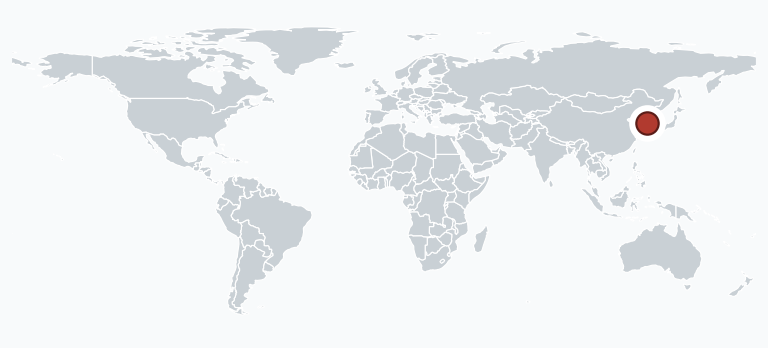
\includegraphics[width=\linewidth,keepaspectratio]{../figures/campus-locators/aifab-008-world-locator.png}
\par\smallskip
{\sffamily\scriptsize Coordinates: 37.219, 127.066.\par}
{\sffamily\scriptsize\color{black!68} Coordinates are the representative point returned for the cited OpenStreetMap feature.\nobreak\textsuperscript{\href{\detokenize{https://www.openstreetmap.org/way/479889842}}{\textcolor{accent}{1}}}\par}
\end{minipage}
\par\vspace{0.9em}
\noindent
\begin{minipage}[t]{\textwidth}
\raggedright
% Image-left evidence-right profile row
\begin{minipage}[t]{0.64\textwidth}
\vspace{0pt}\raggedright
\includegraphics[width=\linewidth,height=0.42\textheight,keepaspectratio,trim=0 0bp 0 0bp,clip]{../assets/campus-imagery/aifab-008.png}
\end{minipage}
\hfill
\begin{minipage}[t]{0.32\textwidth}
\vspace{0pt}\vspace{1.0em}\raggedright
{\sffamily\scriptsize World Imagery; source imagery dated December 22, 2025; source extract 0.585938 m grid; 2.4 km view. Source: Esri, Vantor, Earthstar Geographics, and the GIS User Community. Local imagery: Vantor Vivid Advanced (WV02), source dated 2025-12-22, Raster Basemaps 2026.R04. Map image is the intellectual property of Esri and is used herein under license. Copyright © 2026 Esri and its licensors. All rights reserved. Cropped and annotated by the authors.\nobreak\textsuperscript{\href{\detokenize{https://www.arcgis.com/home/item.html?id=10df2279f9684e4a9f6a7f08febac2a9}}{\textcolor{accent}{5}}} Yellow cross: cited location point.\par}
\medskip
{\footnotesize Samsung's site materials identify Hwaseong and its 10 nm through 3 nm processes.\nobreak\textsuperscript{\href{\detokenize{https://semiconductor.samsung.com/foundry/manufacturing/manufacturing-sites/}}{\textcolor{accent}{2}},\href{\detokenize{https://semiconductor.samsung.com/news-events/news/samsung-electronics-holds-commemorative-ceremony-for-the-first-3nm-mass-production-shipment/}}{\textcolor{accent}{3}}}\par}
\medskip
{\footnotesize\textbf{Documented wafer-fabrication capability:} 10--3 nm foundry capability per Samsung; 2 nm (SF2) production on the S3 line is independently reported\nobreak\textsuperscript{\href{\detokenize{https://semiconductor.samsung.com/foundry/manufacturing/manufacturing-sites/}}{\textcolor{accent}{2}},\href{\detokenize{https://semiconductor.samsung.com/news-events/news/samsung-electronics-holds-commemorative-ceremony-for-the-first-3nm-mass-production-shipment/}}{\textcolor{accent}{3}},\href{\detokenize{https://www.hankyung.com/article/202602189192i}}{\textcolor{accent}{4}}}\par}
\end{minipage}
\end{minipage}
\par\vspace{0.65em}
\medskip
{\footnotesize\textbf{Named data-center AI accelerators or programs:} None identified in the sources reviewed.\par}
\smallskip
{\sffamily\scriptsize\color{black!62}\textbf{Other public catalogues (same campus; reviewed August 25, 2026):} \href{\detokenize{https://en.wikipedia.org/w/index.php?title=List_of_semiconductor_fabrication_plants&oldid=1370451124}\#\detokenize{Open_plants}}{Wikipedia fab list}; \href{\detokenize{https://github.com/aminalav/chip-sense/blob/93d22afe9e1309a7bebd6c7c96541f069f1d67ac/src/data/fab-sites.json}\#\detokenize{L33-L40}}{Chip Sense}.\par}
\medskip
{\sffamily\scriptsize\setlength{\emergencystretch}{1.5em}\textbf{Sources.} \textsuperscript{1}\,OpenStreetMap contributors. \href{\detokenize{https://www.openstreetmap.org/way/479889842}}{\enquote{Samsung Hwaseong campus mapped area, OSM way 479889842.}} Accessed August 25, 2026; \textsuperscript{2}\,Samsung Electronics. \href{\detokenize{https://semiconductor.samsung.com/foundry/manufacturing/manufacturing-sites/}}{\enquote{Samsung Foundry manufacturing sites.}} Accessed August 11, 2026; \textsuperscript{3}\,Samsung Electronics. \href{\detokenize{https://semiconductor.samsung.com/news-events/news/samsung-electronics-holds-commemorative-ceremony-for-the-first-3nm-mass-production-shipment/}}{\enquote{Samsung Electronics holds commemorative ceremony for the first 3nm mass-production shipment.}} July 25, 2022; \textsuperscript{4}\,Korea Economic Daily. \href{\detokenize{https://www.hankyung.com/article/202602189192i}}{\enquote{[Samsung Electronics' bold gamble: Can the new Galaxy take Apple down a peg?].}} In Korean. February 18, 2026; \textsuperscript{5}\,Esri. \href{\detokenize{https://www.arcgis.com/home/item.html?id=10df2279f9684e4a9f6a7f08febac2a9}}{\enquote{World Imagery.}} Accessed August 23, 2026.\par}
\vfill
\noindent{\color{hairline}\rule{\linewidth}{0.4pt}}\par\smallskip
{\sffamily\scriptsize\color{black!58} Evidence reviewed through August 25, 2026.\par}
\end{minipage}
\clearpage
% Campus profile AIFAB-007
\markright{Pyeongtaek Campus}
\noindent\begin{minipage}[t][0.90\textheight][t]{\textwidth}
\noindent\begin{minipage}[t]{0.69\textwidth}
\raggedright
{\sffamily\bfseries\Large\color{accent} Pyeongtaek Campus\par}
\smallskip
{\sffamily\small\textbf{Operator:} Samsung Electronics\quad \textbf{Location:} Pyeongtaek, Gyeonggi-do, KOR\par}
{\sffamily\footnotesize\color{black!68}\textbf{Facility status:} Operating (as of 2026-08-25)\par}
\end{minipage}
\hfill
\begin{minipage}[t]{0.27\textwidth}
\raggedright
{\sffamily\bfseries\footnotesize World location}\par\smallskip
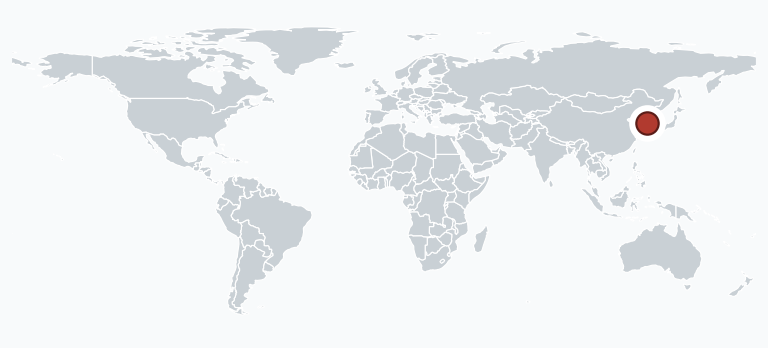
\includegraphics[width=\linewidth,keepaspectratio]{../figures/campus-locators/aifab-007-world-locator.png}
\par\smallskip
{\sffamily\scriptsize Coordinates: 37.036, 127.060.\par}
{\sffamily\scriptsize\color{black!68} Coordinates are the representative point returned for the cited OpenStreetMap feature.\nobreak\textsuperscript{\href{\detokenize{https://www.openstreetmap.org/relation/10723148}}{\textcolor{accent}{1}}}\par}
\end{minipage}
\par\vspace{0.9em}
\noindent
\begin{minipage}[t]{\textwidth}
\raggedright
% Image-left evidence-right profile row
\begin{minipage}[t]{0.64\textwidth}
\vspace{0pt}\raggedright
\includegraphics[width=\linewidth,height=0.42\textheight,keepaspectratio,trim=0 0bp 0 0bp,clip]{../assets/campus-imagery/aifab-007.png}
\end{minipage}
\hfill
\begin{minipage}[t]{0.32\textwidth}
\vspace{0pt}\vspace{1.0em}\raggedright
{\sffamily\scriptsize World Imagery; source imagery dated December 22, 2025; source extract 0.683594 m grid; 2.8 km view. Source: Esri, Vantor, Earthstar Geographics, and the GIS User Community. Local imagery: Vantor Vivid Advanced (WV02), source dated 2025-12-22, Raster Basemaps 2026.R04. Map image is the intellectual property of Esri and is used herein under license. Copyright © 2026 Esri and its licensors. All rights reserved. Cropped and annotated by the authors.\nobreak\textsuperscript{\href{\detokenize{https://www.arcgis.com/home/item.html?id=10df2279f9684e4a9f6a7f08febac2a9}}{\textcolor{accent}{8}}} Yellow cross: cited location point.\par}
\medskip
{\footnotesize Samsung identifies Pyeongtaek as an advanced foundry campus.\nobreak\textsuperscript{\href{\detokenize{https://semiconductor.samsung.com/foundry/manufacturing/manufacturing-sites/}}{\textcolor{accent}{2}},\href{\detokenize{https://semiconductor.samsung.com/news-events/news/samsung-electronics-expands-its-foundry-capacity-with-a-new-production-line-in-pyeongtaek-korea/}}{\textcolor{accent}{3}}}\par}
\medskip
{\footnotesize\textbf{Documented wafer-fabrication capability:} Advanced-node S5 and S6 lines; Samsung's 2020 release planned EUV 5 nm-and-below production; 4 nm output on S5 is independently reported\nobreak\textsuperscript{\href{\detokenize{https://semiconductor.samsung.com/foundry/manufacturing/manufacturing-sites/}}{\textcolor{accent}{2}},\href{\detokenize{https://semiconductor.samsung.com/news-events/news/samsung-electronics-expands-its-foundry-capacity-with-a-new-production-line-in-pyeongtaek-korea/}}{\textcolor{accent}{3}},\href{\detokenize{https://en.sedaily.com/finance/2026/08/25/samsung-foundry-starts-mass-production-of-nvidias-groq3-ai}}{\textcolor{accent}{4}}}\par}
\end{minipage}
\end{minipage}
\par\vspace{0.65em}
\medskip
{\footnotesize\textbf{Named data-center AI accelerators or programs:}\par}
\begin{itemize}[leftmargin=1.25em,itemsep=0.35em,topsep=0.15em,parsep=0pt]
\item {\footnotesize\textbf{NVIDIA --- Groq 3 LPU.} NVIDIA states that Groq 3 LPX is in full production, and Samsung identifies itself as the LPU's manufacturing partner. Independent reporting places 4 nm production on the S5 line at Pyeongtaek P2.\nobreak\textsuperscript{\href{\detokenize{https://semiconductor.samsung.com/foundry/manufacturing/manufacturing-sites/}}{\textcolor{accent}{2}},\href{\detokenize{https://en.sedaily.com/finance/2026/08/25/samsung-foundry-starts-mass-production-of-nvidias-groq3-ai}}{\textcolor{accent}{4}},\href{\detokenize{https://www.asiae.co.kr/en/article/2026032011275710431}}{\textcolor{accent}{5}},\href{\detokenize{https://semiconductor.samsung.com/news-events/tech-blog/architecting-the-ai-era-samsung-electronics-and-nvidia-define-the-future-at-gtc-2026/}}{\textcolor{accent}{6}},\href{\detokenize{https://investor.nvidia.com/news/press-release-details/2026/NVIDIA-Groq-3-LPX-Now-in-Full-Production-With-World-Class-Speed-for-Agentic-AI/default.aspx}}{\textcolor{accent}{7}}}\par {\scriptsize\color{black!62}\textbf{Limits of the evidence:} The first-party sources reviewed do not name the node or campus or state what share is made at Pyeongtaek.\par}}
\end{itemize}
\smallskip
{\sffamily\scriptsize\color{black!62}\textbf{Other public catalogues (same campus; reviewed August 25, 2026):} \href{\detokenize{https://en.wikipedia.org/w/index.php?title=List_of_semiconductor_fabrication_plants&oldid=1370451124}\#\detokenize{Open_plants}}{Wikipedia fab list}.\par}
\medskip
{\sffamily\scriptsize\setlength{\emergencystretch}{1.5em}\textbf{Sources.} \textsuperscript{1}\,OpenStreetMap contributors. \href{\detokenize{https://www.openstreetmap.org/relation/10723148}}{\enquote{Samsung Pyeongtaek campus mapped area, OSM relation 10723148.}} Accessed August 25, 2026; \textsuperscript{2}\,Samsung Electronics. \href{\detokenize{https://semiconductor.samsung.com/foundry/manufacturing/manufacturing-sites/}}{\enquote{Samsung Foundry manufacturing sites.}} Accessed August 11, 2026; \textsuperscript{3}\,Samsung Electronics. \href{\detokenize{https://semiconductor.samsung.com/news-events/news/samsung-electronics-expands-its-foundry-capacity-with-a-new-production-line-in-pyeongtaek-korea/}}{\enquote{Samsung Electronics Expands its Foundry Capacity with A New Production Line in Pyeongtaek, Korea.}} May 22, 2020; \textsuperscript{4}\,Seoul Economic Daily. \href{\detokenize{https://en.sedaily.com/finance/2026/08/25/samsung-foundry-starts-mass-production-of-nvidias-groq3-ai}}{\enquote{Samsung Foundry starts mass production of NVIDIA Groq 3 AI chip.}} August 25, 2026; \textsuperscript{5}\,Asia Economy. \href{\detokenize{https://www.asiae.co.kr/en/article/2026032011275710431}}{\enquote{[Chip Talk] Samsung Foundry Sheds `Loss-Making' Label with Spectacular Comeback... Big Tech Orders Pour In.}} March 21, 2026; \textsuperscript{6}\,Samsung Electronics. \href{\detokenize{https://semiconductor.samsung.com/news-events/tech-blog/architecting-the-ai-era-samsung-electronics-and-nvidia-define-the-future-at-gtc-2026/}}{\enquote{Architecting the AI Era: Samsung Electronics and NVIDIA Define the Future at GTC 2026.}} March 18, 2026; \textsuperscript{7}\,NVIDIA. \href{\detokenize{https://investor.nvidia.com/news/press-release-details/2026/NVIDIA-Groq-3-LPX-Now-in-Full-Production-With-World-Class-Speed-for-Agentic-AI/default.aspx}}{\enquote{NVIDIA Groq 3 LPX now in full production.}} August 24, 2026; \textsuperscript{8}\,Esri. \href{\detokenize{https://www.arcgis.com/home/item.html?id=10df2279f9684e4a9f6a7f08febac2a9}}{\enquote{World Imagery.}} Accessed August 23, 2026.\par}
\vfill
\noindent{\color{hairline}\rule{\linewidth}{0.4pt}}\par\smallskip
{\sffamily\scriptsize\color{black!58} Evidence reviewed through August 25, 2026.\par}
\end{minipage}
\clearpage
% Campus profile AIFAB-018
\markright{JASM Kumamoto campus}
\noindent\begin{minipage}[t][0.90\textheight][t]{\textwidth}
\noindent\begin{minipage}[t]{0.69\textwidth}
\raggedright
{\sffamily\bfseries\Large\color{accent} JASM Kumamoto campus\par}
\smallskip
{\sffamily\small\textbf{Operator:} TSMC / JASM\quad \textbf{Location:} Kikuyo, Kumamoto, JPN\par}
{\sffamily\footnotesize\color{black!68}\textbf{Facility status:} Operating; expansion under construction (as of 2026-08-25)\par}
\end{minipage}
\hfill
\begin{minipage}[t]{0.27\textwidth}
\raggedright
{\sffamily\bfseries\footnotesize World location}\par\smallskip
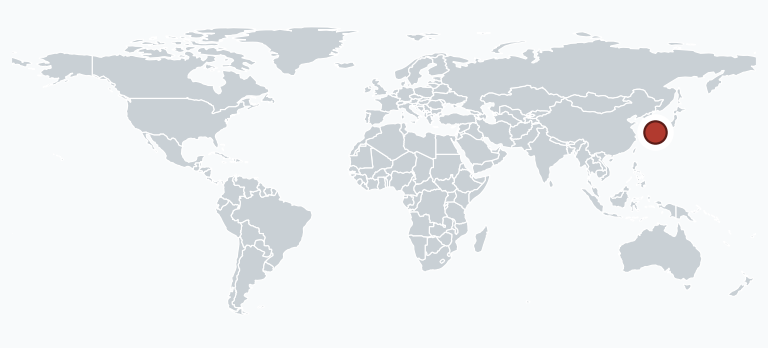
\includegraphics[width=\linewidth,keepaspectratio]{../figures/campus-locators/aifab-018-world-locator.png}
\par\smallskip
{\sffamily\scriptsize Coordinates: 32.887, 130.843.\par}
{\sffamily\scriptsize\color{black!68} Coordinates are the representative point returned for the cited OpenStreetMap feature.\nobreak\textsuperscript{\href{\detokenize{https://www.openstreetmap.org/way/1178207154}}{\textcolor{accent}{1}}}\par}
\end{minipage}
\par\vspace{0.9em}
\noindent
\begin{minipage}[t]{\textwidth}
\raggedright
% Image-left evidence-right profile row
\begin{minipage}[t]{0.64\textwidth}
\vspace{0pt}\raggedright
\includegraphics[width=\linewidth,height=0.42\textheight,keepaspectratio,trim=0 0bp 0 0bp,clip]{../assets/campus-imagery/aifab-018.png}
\end{minipage}
\hfill
\begin{minipage}[t]{0.32\textwidth}
\vspace{0pt}\vspace{1.0em}\raggedright
{\sffamily\scriptsize Created by editing GSI Tiles, `2026 Kumamoto-1 Orthophoto, August 3 Flight,' Geospatial Information Authority of Japan; photographed August 3, 2026; peripheral gaps filled from the GSI seamless aerial photo mosaic; source extract 0.585938 m grid; 2.4 km view.\nobreak\textsuperscript{\href{\detokenize{https://maps.gsi.go.jp/development/ichiran.html}}{\textcolor{accent}{5}}} Yellow cross: cited location point.\par}
\medskip
{\footnotesize TSMC describes Fab 1 and Fab 2 as parts of one Kumamoto campus; its 20-F names JASM's manufacturing entity Fab 23.\nobreak\textsuperscript{\href{\detokenize{https://pr.tsmc.com/english/news/3105}}{\textcolor{accent}{2}},\href{\detokenize{https://investor.tsmc.com/sites/ir/annual-report/2025/2025}\%\detokenize{20TSMC}\%\detokenize{20Annual}\%\detokenize{20Report.E.pdf}}{\textcolor{accent}{3}},\href{\detokenize{https://investor.tsmc.com/sites/ir/sec-filings/2025_20F}\%\detokenize{20Report.pdf}}{\textcolor{accent}{4}}}\par}
\medskip
{\footnotesize\textbf{Documented wafer-fabrication capability:} Fab 1 (TSMC's Fab 23) is operating, with 28 nm its most advanced volume node at end-2025; TSMC says the two-fab site plans to offer 40, 22/28, 12/16, 6/7, and 3 nm, with 3 nm for Fab 2\nobreak\textsuperscript{\href{\detokenize{https://pr.tsmc.com/english/news/3105}}{\textcolor{accent}{2}},\href{\detokenize{https://investor.tsmc.com/sites/ir/annual-report/2025/2025}\%\detokenize{20TSMC}\%\detokenize{20Annual}\%\detokenize{20Report.E.pdf}}{\textcolor{accent}{3}},\href{\detokenize{https://investor.tsmc.com/sites/ir/sec-filings/2025_20F}\%\detokenize{20Report.pdf}}{\textcolor{accent}{4}}}\par}
\end{minipage}
\end{minipage}
\par\vspace{0.65em}
\medskip
{\footnotesize\textbf{Named data-center AI accelerators or programs:} None identified in the sources reviewed.\par}
\smallskip
{\sffamily\scriptsize\color{black!62}\textbf{Other public catalogues (same campus; reviewed August 25, 2026):} \href{\detokenize{https://en.wikipedia.org/w/index.php?title=List_of_semiconductor_fabrication_plants&oldid=1370451124}\#\detokenize{Open_plants}}{Wikipedia fab list}; \href{\detokenize{https://github.com/aminalav/chip-sense/blob/93d22afe9e1309a7bebd6c7c96541f069f1d67ac/src/data/fab-sites.json}\#\detokenize{L23-L30}}{Chip Sense}.\par}
\medskip
{\sffamily\scriptsize\setlength{\emergencystretch}{1.5em}\textbf{Sources.} \textsuperscript{1}\,OpenStreetMap contributors. \href{\detokenize{https://www.openstreetmap.org/way/1178207154}}{\enquote{JASM mapped facility, OSM way 1178207154.}} Accessed August 25, 2026; \textsuperscript{2}\,TSMC. \href{\detokenize{https://pr.tsmc.com/english/news/3105}}{\enquote{JASM Set to Expand in Kumamoto Japan.}} February 6, 2024; \textsuperscript{3}\,TSMC. \href{\detokenize{https://investor.tsmc.com/sites/ir/annual-report/2025/2025}\%\detokenize{20TSMC}\%\detokenize{20Annual}\%\detokenize{20Report.E.pdf}}{\enquote{TSMC 2025 Annual Report.}} March 1, 2026; \textsuperscript{4}\,TSMC. \href{\detokenize{https://investor.tsmc.com/sites/ir/sec-filings/2025_20F}\%\detokenize{20Report.pdf}}{\enquote{2025 Form 20-F.}} April 16, 2026; \textsuperscript{5}\,Geospatial Information Authority of Japan. \href{\detokenize{https://maps.gsi.go.jp/development/ichiran.html}}{\enquote{2026 Kumamoto-1 orthophoto, August 3 flight.}} Accessed August 23, 2026.\par}
\vfill
\noindent{\color{hairline}\rule{\linewidth}{0.4pt}}\par\smallskip
{\sffamily\scriptsize\color{black!58} Evidence reviewed through August 25, 2026.\par}
\end{minipage}
\clearpage
% Campus profile AIFAB-022
\markright{IIM-1}
\noindent\begin{minipage}[t][0.90\textheight][t]{\textwidth}
\noindent\begin{minipage}[t]{0.69\textwidth}
\raggedright
{\sffamily\bfseries\Large\color{accent} IIM-1\par}
\smallskip
{\sffamily\small\textbf{Operator:} Rapidus\quad \textbf{Location:} Chitose, Hokkaido, JPN\par}
{\sffamily\footnotesize\color{black!68}\textbf{Facility status:} Pilot and prototyping line operating (as of 2026-08-25)\par}
\end{minipage}
\hfill
\begin{minipage}[t]{0.27\textwidth}
\raggedright
{\sffamily\bfseries\footnotesize World location}\par\smallskip
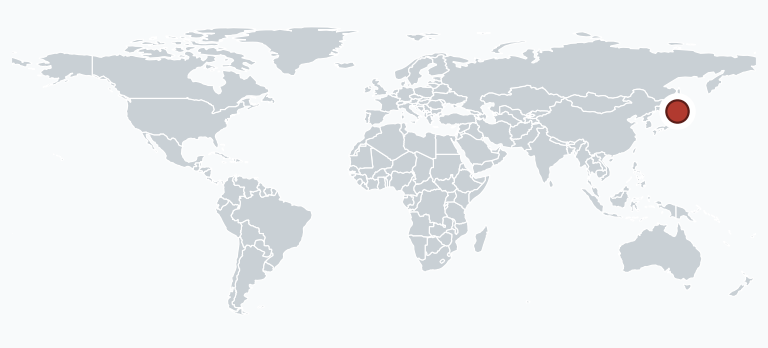
\includegraphics[width=\linewidth,keepaspectratio]{../figures/campus-locators/aifab-022-world-locator.png}
\par\smallskip
{\sffamily\scriptsize Coordinates: 42.787, 141.707.\par}
{\sffamily\scriptsize\color{black!68} Coordinates are the representative point returned for the cited OpenStreetMap feature.\nobreak\textsuperscript{\href{\detokenize{https://www.openstreetmap.org/way/1314075425}}{\textcolor{accent}{1}}}\par}
\end{minipage}
\par\vspace{0.9em}
\noindent
\begin{minipage}[t]{\textwidth}
\raggedright
% Image-left evidence-right profile row
\begin{minipage}[t]{0.64\textwidth}
\vspace{0pt}\raggedright
\includegraphics[width=\linewidth,height=0.42\textheight,keepaspectratio,trim=0 0bp 0 0bp,clip]{../assets/campus-imagery/aifab-022.png}
\end{minipage}
\hfill
\begin{minipage}[t]{0.32\textwidth}
\vspace{0pt}\vspace{1.0em}\raggedright
{\sffamily\scriptsize World Imagery; source imagery dated April 15, 2024; source extract 0.488281 m grid; 2 km view. Source: Esri, Vantor, Earthstar Geographics, and the GIS User Community. Local imagery: Vantor Vivid Advanced (GE01), source dated 2024-04-15, Maps 2024.R08. Map image is the intellectual property of Esri and is used herein under license. Copyright © 2026 Esri and its licensors. All rights reserved. Cropped and annotated by the authors.\nobreak\textsuperscript{\href{\detokenize{https://www.arcgis.com/home/item.html?id=10df2279f9684e4a9f6a7f08febac2a9}}{\textcolor{accent}{4}}} Yellow cross: cited location point.\par}
\medskip
{\footnotesize Rapidus identifies IIM-1 as an operating 2 nm GAA pilot and prototyping site. Commercial mass production remains planned for 2027.\nobreak\textsuperscript{\href{\detokenize{https://www.rapidus.inc/en/iim/}}{\textcolor{accent}{2}},\href{\detokenize{https://www.rapidus.inc/en/news_topics/information/rapidus-achieves-significant-milestone-at-its-state-of-the-art-foundry-with-prototyping-of-leading-edge-2nm-gaa-transistors/}}{\textcolor{accent}{3}}}\par}
\medskip
{\footnotesize\textbf{Documented wafer-fabrication capability:} Operating 2 nm GAA pilot/prototyping line; commercial mass production planned for 2027\nobreak\textsuperscript{\href{\detokenize{https://www.rapidus.inc/en/iim/}}{\textcolor{accent}{2}},\href{\detokenize{https://www.rapidus.inc/en/news_topics/information/rapidus-achieves-significant-milestone-at-its-state-of-the-art-foundry-with-prototyping-of-leading-edge-2nm-gaa-transistors/}}{\textcolor{accent}{3}}}\par}
\end{minipage}
\end{minipage}
\par\vspace{0.65em}
\medskip
{\footnotesize\textbf{Named data-center AI accelerators or programs:} None identified in the sources reviewed.\par}
\medskip
{\sffamily\scriptsize\setlength{\emergencystretch}{1.5em}\textbf{Sources.} \textsuperscript{1}\,OpenStreetMap contributors. \href{\detokenize{https://www.openstreetmap.org/way/1314075425}}{\enquote{Rapidus IIM mapped construction area, OSM way 1314075425.}} Accessed August 11, 2026; \textsuperscript{2}\,Rapidus. \href{\detokenize{https://www.rapidus.inc/en/iim/}}{\enquote{Rapidus Innovative Integration for Manufacturing (IIM-1).}} Accessed August 11, 2026; \textsuperscript{3}\,Rapidus. \href{\detokenize{https://www.rapidus.inc/en/news_topics/information/rapidus-achieves-significant-milestone-at-its-state-of-the-art-foundry-with-prototyping-of-leading-edge-2nm-gaa-transistors/}}{\enquote{Rapidus Achieves Significant Milestone at its State-of-the-Art Foundry with Prototyping of Leading-Edge 2nm GAA Transistors.}} July 18, 2025; \textsuperscript{4}\,Esri. \href{\detokenize{https://www.arcgis.com/home/item.html?id=10df2279f9684e4a9f6a7f08febac2a9}}{\enquote{World Imagery.}} Accessed August 23, 2026.\par}
\vfill
\noindent{\color{hairline}\rule{\linewidth}{0.4pt}}\par\smallskip
{\sffamily\scriptsize\color{black!58} Evidence reviewed through August 25, 2026.\par}
\end{minipage}
\clearpage
% Campus profile AIFAB-023
\markright{Fab 16}
\noindent\begin{minipage}[t][0.90\textheight][t]{\textwidth}
\noindent\begin{minipage}[t]{0.69\textwidth}
\raggedright
{\sffamily\bfseries\Large\color{accent} Fab 16\par}
\smallskip
{\sffamily\small\textbf{Operator:} TSMC\quad \textbf{Location:} Nanjing, Jiangsu, CHN\par}
{\sffamily\footnotesize\color{black!68}\textbf{Facility status:} Operating (as of 2026-08-25)\par}
\end{minipage}
\hfill
\begin{minipage}[t]{0.27\textwidth}
\raggedright
{\sffamily\bfseries\footnotesize World location}\par\smallskip
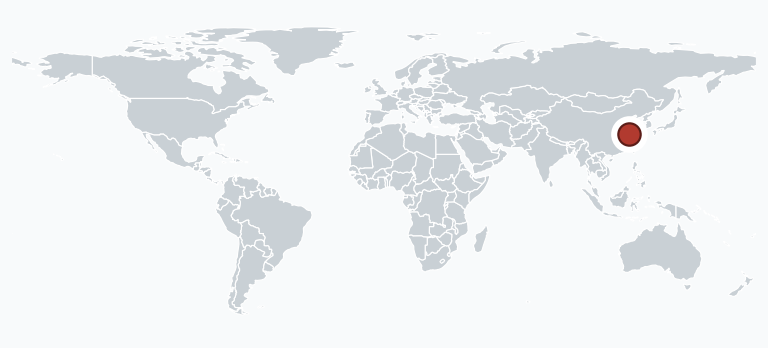
\includegraphics[width=\linewidth,keepaspectratio]{../figures/campus-locators/aifab-023-world-locator.png}
\par\smallskip
{\sffamily\scriptsize Coordinates: 31.976, 118.534.\par}
{\sffamily\scriptsize\color{black!68} Coordinates are the representative point returned for the cited OpenStreetMap feature.\nobreak\textsuperscript{\href{\detokenize{https://www.openstreetmap.org/way/810445179}}{\textcolor{accent}{1}}}\par}
\end{minipage}
\par\vspace{0.9em}
\noindent
\begin{minipage}[t]{\textwidth}
\raggedright
% Image-left evidence-right profile row
\begin{minipage}[t]{0.64\textwidth}
\vspace{0pt}\raggedright
\includegraphics[width=\linewidth,height=0.42\textheight,keepaspectratio,trim=0 0bp 0 0bp,clip]{../assets/campus-imagery/aifab-023.png}
\end{minipage}
\hfill
\begin{minipage}[t]{0.32\textwidth}
\vspace{0pt}\vspace{1.0em}\raggedright
{\sffamily\scriptsize World Imagery; source imagery dated January 1, 2024; source extract 0.488281 m grid; 2 km view. Source: Esri, Vantor, Earthstar Geographics, and the GIS User Community. Local imagery: Vantor Vivid Advanced (WV02), source dated 2024-01-01, Maps 2024.R13. Map image is the intellectual property of Esri and is used herein under license. Copyright © 2026 Esri and its licensors. All rights reserved. Cropped and annotated by the authors.\nobreak\textsuperscript{\href{\detokenize{https://www.arcgis.com/home/item.html?id=10df2279f9684e4a9f6a7f08febac2a9}}{\textcolor{accent}{4}}} Yellow cross: cited location point.\par}
\medskip
{\footnotesize TSMC identifies Fab 16 as an operating campus whose most advanced volume-production technology is 16 nm. TSMC has also announced a 28 nm capacity expansion at the campus.\nobreak\textsuperscript{\href{\detokenize{https://investor.tsmc.com/sites/ir/sec-filings/2025_20F}\%\detokenize{20Report.pdf}}{\textcolor{accent}{2}},\href{\detokenize{https://investor.tsmc.com/chinese/encrypt/files/encrypt_file/reports/2021-10/44ec4960f6771366a2b992ace4ae47566d7206a6/TSMC}\%\detokenize{202Q21}\%\detokenize{20transcript.pdf}}{\textcolor{accent}{3}}}\par}
\medskip
{\footnotesize\textbf{Documented wafer-fabrication capability:} Operating campus whose most advanced volume-production technology is 16 nm; 28 nm capacity expansion also announced\nobreak\textsuperscript{\href{\detokenize{https://investor.tsmc.com/sites/ir/sec-filings/2025_20F}\%\detokenize{20Report.pdf}}{\textcolor{accent}{2}},\href{\detokenize{https://investor.tsmc.com/chinese/encrypt/files/encrypt_file/reports/2021-10/44ec4960f6771366a2b992ace4ae47566d7206a6/TSMC}\%\detokenize{202Q21}\%\detokenize{20transcript.pdf}}{\textcolor{accent}{3}}}\par}
\end{minipage}
\end{minipage}
\par\vspace{0.65em}
\medskip
{\footnotesize\textbf{Named data-center AI accelerators or programs:} None identified in the sources reviewed.\par}
\medskip
{\sffamily\scriptsize\setlength{\emergencystretch}{1.5em}\textbf{Sources.} \textsuperscript{1}\,OpenStreetMap contributors. \href{\detokenize{https://www.openstreetmap.org/way/810445179}}{\enquote{TSMC Fab 16 mapped campus, OSM way 810445179.}} Accessed August 11, 2026; \textsuperscript{2}\,TSMC. \href{\detokenize{https://investor.tsmc.com/sites/ir/sec-filings/2025_20F}\%\detokenize{20Report.pdf}}{\enquote{2025 Form 20-F.}} April 16, 2026; \textsuperscript{3}\,TSMC. \href{\detokenize{https://investor.tsmc.com/chinese/encrypt/files/encrypt_file/reports/2021-10/44ec4960f6771366a2b992ace4ae47566d7206a6/TSMC}\%\detokenize{202Q21}\%\detokenize{20transcript.pdf}}{\enquote{Second Quarter 2021 Earnings Conference Transcript.}} July 15, 2021; \textsuperscript{4}\,Esri. \href{\detokenize{https://www.arcgis.com/home/item.html?id=10df2279f9684e4a9f6a7f08febac2a9}}{\enquote{World Imagery.}} Accessed August 23, 2026.\par}
\vfill
\noindent{\color{hairline}\rule{\linewidth}{0.4pt}}\par\smallskip
{\sffamily\scriptsize\color{black!58} Evidence reviewed through August 25, 2026.\par}
\end{minipage}
\clearpage
% Campus profile AIFAB-009
\markright{SMIC Southern SN1/SN2 campus}
\noindent\begin{minipage}[t][0.90\textheight][t]{\textwidth}
\noindent\begin{minipage}[t]{0.69\textwidth}
\raggedright
{\sffamily\bfseries\Large\color{accent} SMIC Southern SN1/SN2 campus\par}
\smallskip
{\sffamily\small\textbf{Operator:} SMIC\quad \textbf{Location:} Shanghai, CHN\par}
{\sffamily\footnotesize\color{black!68}\textbf{Facility status:} Operating (as of 2026-08-25)\par}
\end{minipage}
\hfill
\begin{minipage}[t]{0.27\textwidth}
\raggedright
{\sffamily\bfseries\footnotesize World location}\par\smallskip
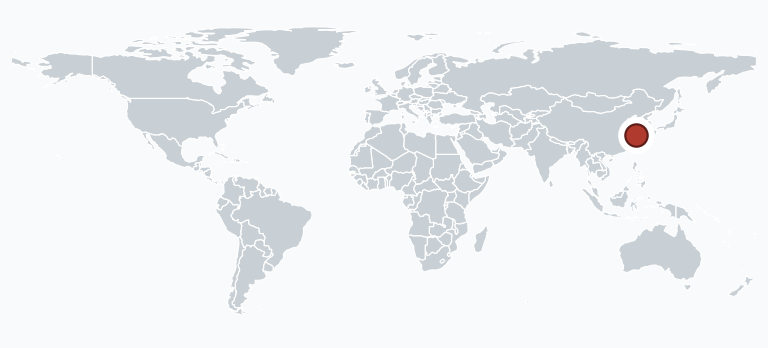
\includegraphics[width=\linewidth,keepaspectratio]{../figures/campus-locators/aifab-009-world-locator.png}
\par\smallskip
{\sffamily\scriptsize Coordinates: 31.217, 121.602.\par}
{\sffamily\scriptsize\color{black!68} Coordinates are the representative point returned for the cited OpenStreetMap feature.\nobreak\textsuperscript{\href{\detokenize{https://www.openstreetmap.org/way/300654142}}{\textcolor{accent}{1}}}\par}
\end{minipage}
\par\vspace{0.9em}
\noindent
\begin{minipage}[t]{\textwidth}
\raggedright
% Image-left evidence-right profile row
\begin{minipage}[t]{0.64\textwidth}
\vspace{0pt}\raggedright
\includegraphics[width=\linewidth,height=0.42\textheight,keepaspectratio,trim=0 0bp 0 0bp,clip]{../assets/campus-imagery/aifab-009.png}
\end{minipage}
\hfill
\begin{minipage}[t]{0.32\textwidth}
\vspace{0pt}\vspace{1.0em}\raggedright
{\sffamily\scriptsize World Imagery; source imagery dated April 18, 2025; source extract 0.488281 m grid; 2 km view. Source: Esri, Vantor, Earthstar Geographics, and the GIS User Community. Local imagery: Vantor Vivid Advanced (WV03), source dated 2025-04-18, Raster Basemaps 2025.R10. Map image is the intellectual property of Esri and is used herein under license. Copyright © 2026 Esri and its licensors. All rights reserved. Cropped and annotated by the authors.\nobreak\textsuperscript{\href{\detokenize{https://www.arcgis.com/home/item.html?id=10df2279f9684e4a9f6a7f08febac2a9}}{\textcolor{accent}{8}}} Yellow cross: cited location point.\par}
\medskip
{\footnotesize A planning record places SN1/SN2 on the Zhangjiang Road block that also holds SMIC's Shanghai 200 mm and 300 mm fabs.\nobreak\textsuperscript{\href{\detokenize{https://www.congress.gov/119/meeting/house/118111/witnesses/HMTG-119-SY15-Wstate-AllenG-20250408.pdf}}{\textcolor{accent}{2}},\href{\detokenize{https://www.pudong.gov.cn/zwgk/14496.gkml_ywl_czxx_czyjs_kfqgwh_zjyqgwh_shszjkxcjsglbgsbb/2022/301/252143.html}}{\textcolor{accent}{3}},\href{\detokenize{https://www1.hkexnews.hk/listedco/listconews/sehk/2020/0608/2020060801093_c.pdf}}{\textcolor{accent}{4}},\href{\detokenize{https://web.archive.org/web/20260514171941/https://www.smics.com/en/site/factory_summary}}{\textcolor{accent}{5}}}\par}
\medskip
{\footnotesize\textbf{Documented wafer-fabrication capability:} 14 nm at SN1; 7 nm-class (N+2) at SN2\nobreak\textsuperscript{\href{\detokenize{https://www.congress.gov/119/meeting/house/118111/witnesses/HMTG-119-SY15-Wstate-AllenG-20250408.pdf}}{\textcolor{accent}{2}},\href{\detokenize{https://www1.hkexnews.hk/listedco/listconews/sehk/2020/0608/2020060801093_c.pdf}}{\textcolor{accent}{4}}}\par}
\end{minipage}
\end{minipage}
\par\vspace{0.65em}
\medskip
{\footnotesize\textbf{Named data-center AI accelerators or programs:}\par}
\begin{itemize}[leftmargin=1.25em,itemsep=0.35em,topsep=0.15em,parsep=0pt]
\item {\footnotesize\textbf{Huawei --- Ascend 910B.} April 2025 congressional testimony reports SMIC producing Ascend 910B dies and calls SN2 China's only active 7 nm line.\nobreak\textsuperscript{\href{\detokenize{https://www.congress.gov/119/meeting/house/118111/witnesses/HMTG-119-SY15-Wstate-AllenG-20250408.pdf}}{\textcolor{accent}{2}},\href{\detokenize{https://cset.georgetown.edu/publication/pushing-the-limits-huaweis-ai-chip-tests-u-s-export-controls/}}{\textcolor{accent}{6}},\href{\detokenize{https://www.malaymail.com/news/money/2024/10/27/tsmc-suspended-shipments-to-china-firm-after-chip-found-on-huawei-processor-sources-say/155003}}{\textcolor{accent}{7}}}\par {\scriptsize\color{black!62}\textbf{Limits of the evidence:} The testimony links the dies to SN2 only by combining these statements; it also cites officials as saying TSMC made over 2 million 910B dies. The sources reviewed do not confirm production after April 2025.\par}}
\end{itemize}
\smallskip
{\sffamily\scriptsize\color{black!62}\textbf{Other public catalogues (same campus; reviewed August 25, 2026):} \href{\detokenize{https://en.wikipedia.org/w/index.php?title=List_of_semiconductor_fabrication_plants&oldid=1370451124}\#\detokenize{Open_plants}}{Wikipedia fab list}.\par}
\medskip
{\sffamily\scriptsize\setlength{\emergencystretch}{1.5em}\textbf{Sources.} \textsuperscript{1}\,OpenStreetMap contributors. \href{\detokenize{https://www.openstreetmap.org/way/300654142}}{\enquote{SMIC mapped industrial area, OSM way 300654142.}} Accessed August 25, 2026; \textsuperscript{2}\,Gregory C. Allen, testimony to the House Committee on Science, Space, and Technology. \href{\detokenize{https://www.congress.gov/119/meeting/house/118111/witnesses/HMTG-119-SY15-Wstate-AllenG-20250408.pdf}}{\enquote{DeepSeek: A Deep Dive.}} April 8, 2025; \textsuperscript{3}\,Zhangjiang Science City Construction Management Office. \href{\detokenize{https://www.pudong.gov.cn/zwgk/14496.gkml_ywl_czxx_czyjs_kfqgwh_zjyqgwh_shszjkxcjsglbgsbb/2022/301/252143.html}}{\enquote{SMIC 12-inch chip SN1 and SN2 plant project (SN2 plant).}} February 14, 2022; \textsuperscript{4}\,SMIC. \href{\detokenize{https://www1.hkexnews.hk/listedco/listconews/sehk/2020/0608/2020060801093_c.pdf}}{\enquote{Overseas Regulatory Announcement (STAR Market IPO review-inquiry reply).}} June 8, 2020; \textsuperscript{5}\,SMIC. \href{\detokenize{https://web.archive.org/web/20260514171941/https://www.smics.com/en/site/factory_summary}}{\enquote{Fab Information.}} Archived May 14, 2026; \textsuperscript{6}\,Center for Security and Emerging Technology. \href{\detokenize{https://cset.georgetown.edu/publication/pushing-the-limits-huaweis-ai-chip-tests-u-s-export-controls/}}{\enquote{Pushing the Limits: Huawei's AI Chip Tests U.S. Export Controls.}} June 17, 2024; \textsuperscript{7}\,Reuters via Malay Mail. \href{\detokenize{https://www.malaymail.com/news/money/2024/10/27/tsmc-suspended-shipments-to-china-firm-after-chip-found-on-huawei-processor-sources-say/155003}}{\enquote{TSMC suspended shipments to China firm after chip found on Huawei processor, sources say.}} October 27, 2024; \textsuperscript{8}\,Esri. \href{\detokenize{https://www.arcgis.com/home/item.html?id=10df2279f9684e4a9f6a7f08febac2a9}}{\enquote{World Imagery.}} Accessed August 23, 2026.\par}
\vfill
\noindent{\color{hairline}\rule{\linewidth}{0.4pt}}\par\smallskip
{\sffamily\scriptsize\color{black!58} Evidence reviewed through August 25, 2026.\par}
\end{minipage}
\clearpage
% Campus profile AIFAB-029
\markright{Shenzhen Pingshan campus}
\noindent\begin{minipage}[t][0.90\textheight][t]{\textwidth}
\noindent\begin{minipage}[t]{0.69\textwidth}
\raggedright
{\sffamily\bfseries\Large\color{accent} Shenzhen Pingshan campus\par}
\smallskip
{\sffamily\small\textbf{Operator:} SMIC\quad \textbf{Location:} Shenzhen, Guangdong, CHN\par}
{\sffamily\footnotesize\color{black!68}\textbf{Facility status:} Operating (as of 2026-08-11)\par}
\end{minipage}
\hfill
\begin{minipage}[t]{0.27\textwidth}
\raggedright
{\sffamily\bfseries\footnotesize World location}\par\smallskip
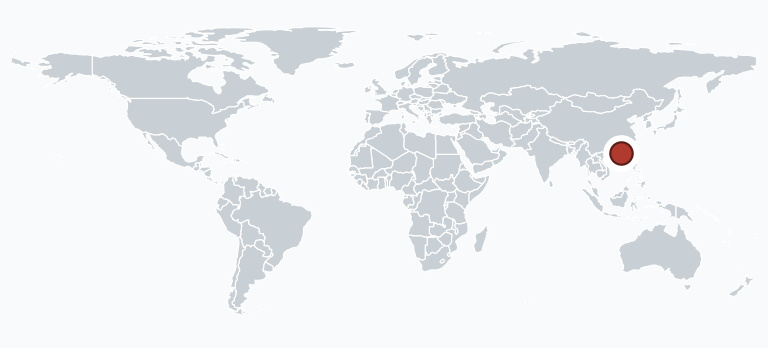
\includegraphics[width=\linewidth,keepaspectratio]{../figures/campus-locators/aifab-029-world-locator.png}
\par\smallskip
{\sffamily\scriptsize Coordinates: 22.716, 114.354.\par}
{\sffamily\scriptsize\color{black!68} Coordinates are the representative point returned for the cited OpenStreetMap feature.\nobreak\textsuperscript{\href{\detokenize{https://www.openstreetmap.org/way/797826476}}{\textcolor{accent}{1}}}\par}
\end{minipage}
\par\vspace{0.9em}
\noindent
\begin{minipage}[t]{\textwidth}
\raggedright
% Image-left evidence-right profile row
\begin{minipage}[t]{0.64\textwidth}
\vspace{0pt}\raggedright
\includegraphics[width=\linewidth,height=0.42\textheight,keepaspectratio,trim=0 0bp 0 0bp,clip]{../assets/campus-imagery/aifab-029.png}
\end{minipage}
\hfill
\begin{minipage}[t]{0.32\textwidth}
\vspace{0pt}\vspace{1.0em}\raggedright
{\sffamily\scriptsize World Imagery; source imagery dates September 16, 2022 and September 15, 2024; source extract 0.488281 m grid; 2 km view. Source: Esri, Vantor, Earthstar Geographics, and the GIS User Community. Local imagery: Vantor Vivid Advanced (GE01), source dated 2022-09-16, Raster Basemaps 2025.R06; Vantor Vivid Advanced (WV03), source dated 2024-09-15, Raster Basemaps 2025.R06. Map image is the intellectual property of Esri and is used herein under license. Copyright © 2026 Esri and its licensors. All rights reserved. Cropped and annotated by the authors.\nobreak\textsuperscript{\href{\detokenize{https://www.arcgis.com/home/item.html?id=10df2279f9684e4a9f6a7f08febac2a9}}{\textcolor{accent}{4}}} Yellow cross: cited location point.\par}
\medskip
{\footnotesize Public sources identify the Pingshan campus as an operating mature-node production site.\nobreak\textsuperscript{\href{\detokenize{https://www1.hkexnews.hk/listedco/listconews/sehk/2026/0408/2026040801181.pdf}}{\textcolor{accent}{2}},\href{\detokenize{https://www.szpsq.gov.cn/english/From}\%\detokenize{20Pingshan}\%\detokenize{20to}\%\detokenize{20the}\%\detokenize{20World/Key}\%\detokenize{20Industries}\%\detokenize{20amp}\%\detokenize{3Bamp}\%\detokenize{3Bamp}\%\detokenize{3B}\%\detokenize{20Bonded}\%\detokenize{20Zone/content/post_10912456.html}}{\textcolor{accent}{3}}}\par}
\medskip
{\footnotesize\textbf{Documented wafer-fabrication capability:} Pingshan District states that the first 12-inch phase entered production in June 2022 and focuses on 28 nm-and-above ICs; it also identifies an expanded 8-inch line at the site.\nobreak\textsuperscript{\href{\detokenize{https://www.szpsq.gov.cn/english/From}\%\detokenize{20Pingshan}\%\detokenize{20to}\%\detokenize{20the}\%\detokenize{20World/Key}\%\detokenize{20Industries}\%\detokenize{20amp}\%\detokenize{3Bamp}\%\detokenize{3Bamp}\%\detokenize{3B}\%\detokenize{20Bonded}\%\detokenize{20Zone/content/post_10912456.html}}{\textcolor{accent}{3}}}\par}
\end{minipage}
\end{minipage}
\par\vspace{0.65em}
\medskip
{\footnotesize\textbf{Named data-center AI accelerators or programs:} None identified in the sources reviewed.\par}
\smallskip
{\sffamily\scriptsize\color{black!62}\textbf{Other public catalogues (same campus; reviewed August 25, 2026):} \href{\detokenize{https://en.wikipedia.org/w/index.php?title=List_of_semiconductor_fabrication_plants&oldid=1370451124}\#\detokenize{Open_plants}}{Wikipedia fab list}.\par}
\medskip
{\sffamily\scriptsize\setlength{\emergencystretch}{1.5em}\textbf{Sources.} \textsuperscript{1}\,OpenStreetMap contributors. \href{\detokenize{https://www.openstreetmap.org/way/797826476}}{\enquote{SMIC Shenzhen Pingshan mapped campus, OSM way 797826476.}} Accessed August 11, 2026; \textsuperscript{2}\,SMIC. \href{\detokenize{https://www1.hkexnews.hk/listedco/listconews/sehk/2026/0408/2026040801181.pdf}}{\enquote{SMIC 2025 Annual Report.}} April 8, 2026; \textsuperscript{3}\,People's Government of Pingshan District. \href{\detokenize{https://www.szpsq.gov.cn/english/From}\%\detokenize{20Pingshan}\%\detokenize{20to}\%\detokenize{20the}\%\detokenize{20World/Key}\%\detokenize{20Industries}\%\detokenize{20amp}\%\detokenize{3Bamp}\%\detokenize{3Bamp}\%\detokenize{3B}\%\detokenize{20Bonded}\%\detokenize{20Zone/content/post_10912456.html}}{\enquote{New-generation information technology and intelligent manufacturing industry.}} October 27, 2023; \textsuperscript{4}\,Esri. \href{\detokenize{https://www.arcgis.com/home/item.html?id=10df2279f9684e4a9f6a7f08febac2a9}}{\enquote{World Imagery.}} Accessed August 23, 2026.\par}
\vfill
\noindent{\color{hairline}\rule{\linewidth}{0.4pt}}\par\smallskip
{\sffamily\scriptsize\color{black!58} Evidence reviewed through August 25, 2026.\par}
\end{minipage}
\clearpage
% Campus profile AIFAB-028
\markright{Beijing Jingcheng campus}
\noindent\begin{minipage}[t][0.90\textheight][t]{\textwidth}
\noindent\begin{minipage}[t]{0.69\textwidth}
\raggedright
{\sffamily\bfseries\Large\color{accent} Beijing Jingcheng campus\par}
\smallskip
{\sffamily\small\textbf{Operator:} SMIC / SMBC\quad \textbf{Location:} Beijing, CHN\par}
{\sffamily\footnotesize\color{black!68}\textbf{Facility status:} Operating (as of 2026-08-24)\par}
\end{minipage}
\hfill
\begin{minipage}[t]{0.27\textwidth}
\raggedright
{\sffamily\bfseries\footnotesize World location}\par\smallskip
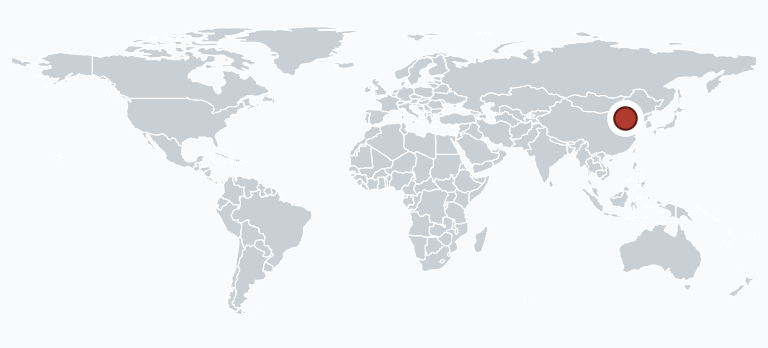
\includegraphics[width=\linewidth,keepaspectratio]{../figures/campus-locators/aifab-028-world-locator.png}
\par\smallskip
{\sffamily\scriptsize Coordinates: 39.727, 116.572.\par}
{\sffamily\scriptsize\color{black!68} Coordinates estimate the center of the four-road parcel described in the cited sources.\nobreak\textsuperscript{\href{\detokenize{https://www.smics.com/uploads/6795f77a/}\%\detokenize{26e8}\%\detokenize{2687}\%\detokenize{26aa}\%\detokenize{26e8}\%\detokenize{26a1}\%\detokenize{268c}\%\detokenize{26e7}\%\detokenize{269b}\%\detokenize{2691}\%\detokenize{26e6}\%\detokenize{26b5}\%\detokenize{268b}\%\detokenize{26e5}\%\detokenize{26b9}\%\detokenize{26b4}\%\detokenize{26e5}\%\detokenize{26ba}\%\detokenize{26a6}\%\detokenize{26e6}\%\detokenize{268a}\%\detokenize{26a5}\%\detokenize{26e5}\%\detokenize{2691}\%\detokenize{268a2024}\%\detokenize{26e5}\%\detokenize{26b9}\%\detokenize{26b4.pdf}}{\textcolor{accent}{1}}}\par}
\end{minipage}
\par\vspace{0.9em}
\noindent
\begin{minipage}[t]{\textwidth}
\raggedright
% Image-left evidence-right profile row
\begin{minipage}[t]{0.64\textwidth}
\vspace{0pt}\raggedright
\includegraphics[width=\linewidth,height=0.42\textheight,keepaspectratio,trim=0 0bp 0 0bp,clip]{../assets/campus-imagery/aifab-028.png}
\end{minipage}
\hfill
\begin{minipage}[t]{0.32\textwidth}
\vspace{0pt}\vspace{1.0em}\raggedright
{\sffamily\scriptsize World Imagery; source imagery dated January 11, 2026; source extract 0.488281 m grid; 2 km view. Source: Esri, Vantor, Earthstar Geographics, and the GIS User Community. Local imagery: Vantor Vivid Advanced (WV02), source dated 2026-01-11, Raster Basemaps 2026.R06. Map image is the intellectual property of Esri and is used herein under license. Copyright © 2026 Esri and its licensors. All rights reserved. Cropped and annotated by the authors.\nobreak\textsuperscript{\href{\detokenize{https://www.arcgis.com/home/item.html?id=10df2279f9684e4a9f6a7f08febac2a9}}{\textcolor{accent}{5}}} Yellow cross: cited location point.\par}
\medskip
{\footnotesize Exact-campus environmental records identify 12-inch fabrication at 28 nm and larger process nodes and report production on all 365 days of 2024.\nobreak\textsuperscript{\href{\detokenize{https://www.smics.com/uploads/6795f77a/}\%\detokenize{26e8}\%\detokenize{2687}\%\detokenize{26aa}\%\detokenize{26e8}\%\detokenize{26a1}\%\detokenize{268c}\%\detokenize{26e7}\%\detokenize{269b}\%\detokenize{2691}\%\detokenize{26e6}\%\detokenize{26b5}\%\detokenize{268b}\%\detokenize{26e5}\%\detokenize{26b9}\%\detokenize{26b4}\%\detokenize{26e5}\%\detokenize{26ba}\%\detokenize{26a6}\%\detokenize{26e6}\%\detokenize{268a}\%\detokenize{26a5}\%\detokenize{26e5}\%\detokenize{2691}\%\detokenize{268a2024}\%\detokenize{26e5}\%\detokenize{26b9}\%\detokenize{26b4.pdf}}{\textcolor{accent}{1}},\href{\detokenize{https://www1.hkexnews.hk/listedco/listconews/sehk/2026/0408/2026040801181.pdf}}{\textcolor{accent}{2}},\href{\detokenize{https://www1.hkexnews.hk/listedco/listconews/sehk/2020/1204/2020120401701.pdf}}{\textcolor{accent}{3}},\href{\detokenize{https://www.smics.com/uploads/2025}\%\detokenize{26e5}\%\detokenize{26b9}\%\detokenize{26b4}\%\detokenize{26e8}\%\detokenize{2687}\%\detokenize{26aa}\%\detokenize{26e8}\%\detokenize{26a1}\%\detokenize{268c}\%\detokenize{26e7}\%\detokenize{269b}\%\detokenize{2691}\%\detokenize{26e6}\%\detokenize{26b5}\%\detokenize{268b}\%\detokenize{26e6}\%\detokenize{2696}\%\detokenize{26b9}\%\detokenize{26e6}\%\detokenize{26a1}\%\detokenize{2688.pdf}}{\textcolor{accent}{4}}}\par}
\medskip
{\footnotesize\textbf{Documented wafer-fabrication capability:} Operating 12-inch manufacturing at 28 nm and larger process nodes\nobreak\textsuperscript{\href{\detokenize{https://www.smics.com/uploads/6795f77a/}\%\detokenize{26e8}\%\detokenize{2687}\%\detokenize{26aa}\%\detokenize{26e8}\%\detokenize{26a1}\%\detokenize{268c}\%\detokenize{26e7}\%\detokenize{269b}\%\detokenize{2691}\%\detokenize{26e6}\%\detokenize{26b5}\%\detokenize{268b}\%\detokenize{26e5}\%\detokenize{26b9}\%\detokenize{26b4}\%\detokenize{26e5}\%\detokenize{26ba}\%\detokenize{26a6}\%\detokenize{26e6}\%\detokenize{268a}\%\detokenize{26a5}\%\detokenize{26e5}\%\detokenize{2691}\%\detokenize{268a2024}\%\detokenize{26e5}\%\detokenize{26b9}\%\detokenize{26b4.pdf}}{\textcolor{accent}{1}},\href{\detokenize{https://www1.hkexnews.hk/listedco/listconews/sehk/2020/1204/2020120401701.pdf}}{\textcolor{accent}{3}},\href{\detokenize{https://www.smics.com/uploads/2025}\%\detokenize{26e5}\%\detokenize{26b9}\%\detokenize{26b4}\%\detokenize{26e8}\%\detokenize{2687}\%\detokenize{26aa}\%\detokenize{26e8}\%\detokenize{26a1}\%\detokenize{268c}\%\detokenize{26e7}\%\detokenize{269b}\%\detokenize{2691}\%\detokenize{26e6}\%\detokenize{26b5}\%\detokenize{268b}\%\detokenize{26e6}\%\detokenize{2696}\%\detokenize{26b9}\%\detokenize{26e6}\%\detokenize{26a1}\%\detokenize{2688.pdf}}{\textcolor{accent}{4}}}\par}
\end{minipage}
\end{minipage}
\par\vspace{0.65em}
\medskip
{\footnotesize\textbf{Named data-center AI accelerators or programs:} None identified in the sources reviewed.\par}
\smallskip
{\sffamily\scriptsize\color{black!62}\textbf{Other public catalogues (same campus; reviewed August 25, 2026):} \href{\detokenize{https://en.wikipedia.org/w/index.php?title=List_of_semiconductor_fabrication_plants&oldid=1370451124}\#\detokenize{Open_plants}}{Wikipedia fab list}.\par}
\medskip
{\sffamily\scriptsize\setlength{\emergencystretch}{1.5em}\textbf{Sources.} \textsuperscript{1}\,Semiconductor Manufacturing Beijing Corporation. \href{\detokenize{https://www.smics.com/uploads/6795f77a/}\%\detokenize{26e8}\%\detokenize{2687}\%\detokenize{26aa}\%\detokenize{26e8}\%\detokenize{26a1}\%\detokenize{268c}\%\detokenize{26e7}\%\detokenize{269b}\%\detokenize{2691}\%\detokenize{26e6}\%\detokenize{26b5}\%\detokenize{268b}\%\detokenize{26e5}\%\detokenize{26b9}\%\detokenize{26b4}\%\detokenize{26e5}\%\detokenize{26ba}\%\detokenize{26a6}\%\detokenize{26e6}\%\detokenize{268a}\%\detokenize{26a5}\%\detokenize{26e5}\%\detokenize{2691}\%\detokenize{268a2024}\%\detokenize{26e5}\%\detokenize{26b9}\%\detokenize{26b4.pdf}}{\enquote{2024 Annual Self-Monitoring Report.}} January 23, 2025; \textsuperscript{2}\,SMIC. \href{\detokenize{https://www1.hkexnews.hk/listedco/listconews/sehk/2026/0408/2026040801181.pdf}}{\enquote{SMIC 2025 Annual Report.}} April 8, 2026; \textsuperscript{3}\,SMIC. \href{\detokenize{https://www1.hkexnews.hk/listedco/listconews/sehk/2020/1204/2020120401701.pdf}}{\enquote{Formation of Joint Venture Company in Beijing.}} December 4, 2020; \textsuperscript{4}\,Semiconductor Manufacturing Beijing Corporation. \href{\detokenize{https://www.smics.com/uploads/2025}\%\detokenize{26e5}\%\detokenize{26b9}\%\detokenize{26b4}\%\detokenize{26e8}\%\detokenize{2687}\%\detokenize{26aa}\%\detokenize{26e8}\%\detokenize{26a1}\%\detokenize{268c}\%\detokenize{26e7}\%\detokenize{269b}\%\detokenize{2691}\%\detokenize{26e6}\%\detokenize{26b5}\%\detokenize{268b}\%\detokenize{26e6}\%\detokenize{2696}\%\detokenize{26b9}\%\detokenize{26e6}\%\detokenize{26a1}\%\detokenize{2688.pdf}}{\enquote{2025 Self-Monitoring Plan.}} 2025; \textsuperscript{5}\,Esri. \href{\detokenize{https://www.arcgis.com/home/item.html?id=10df2279f9684e4a9f6a7f08febac2a9}}{\enquote{World Imagery.}} Accessed September 27, 2026.\par}
\vfill
\noindent{\color{hairline}\rule{\linewidth}{0.4pt}}\par\smallskip
{\sffamily\scriptsize\color{black!58} Evidence reviewed through August 25, 2026.\par}
\end{minipage}
\clearpage
% Campus profile AIFAB-030
\markright{Shanghai Lingang campus}
\noindent\begin{minipage}[t][0.90\textheight][t]{\textwidth}
\noindent\begin{minipage}[t]{0.69\textwidth}
\raggedright
{\sffamily\bfseries\Large\color{accent} Shanghai Lingang campus\par}
\smallskip
{\sffamily\small\textbf{Operator:} SMIC / SMOC\quad \textbf{Location:} Shanghai, CHN\par}
{\sffamily\footnotesize\color{black!68}\textbf{Facility status:} Operating (as of 2026-08-25)\par}
\end{minipage}
\hfill
\begin{minipage}[t]{0.27\textwidth}
\raggedright
{\sffamily\bfseries\footnotesize World location}\par\smallskip
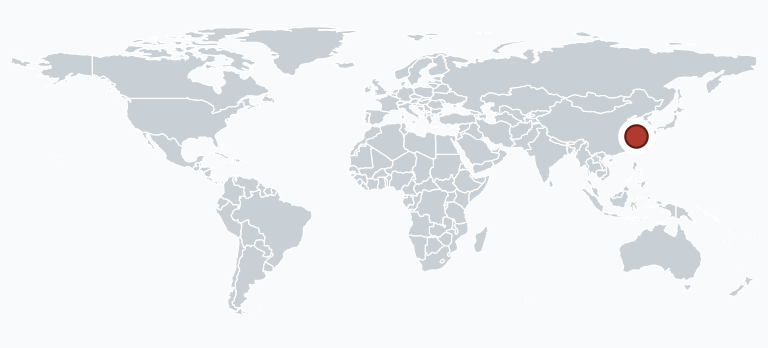
\includegraphics[width=\linewidth,keepaspectratio]{../figures/campus-locators/aifab-030-world-locator.png}
\par\smallskip
{\sffamily\scriptsize Coordinates: 30.987, 121.837.\par}
{\sffamily\scriptsize\color{black!68} Converted (GCJ-02 assumed) from an SMIC Lingang project's environmental record, which does not tie the point to this campus.\nobreak\textsuperscript{\href{\detokenize{https://nanoplatform.cn/new/14147/}}{\textcolor{accent}{1}}}\par}
\end{minipage}
\par\vspace{0.9em}
\noindent
\begin{minipage}[t]{\textwidth}
\raggedright
% Image-left evidence-right profile row
\begin{minipage}[t]{0.64\textwidth}
\vspace{0pt}\raggedright
\includegraphics[width=\linewidth,height=0.42\textheight,keepaspectratio,trim=0 0bp 0 0bp,clip]{../assets/campus-imagery/aifab-030.png}
\end{minipage}
\hfill
\begin{minipage}[t]{0.32\textwidth}
\vspace{0pt}\vspace{1.0em}\raggedright
{\sffamily\scriptsize World Imagery; source imagery dates April 13, 2025, April 15, 2025, and July 4, 2025; source extract 0.683594 m grid; 2.8 km view. Source: Esri, Vantor, Earthstar Geographics, and the GIS User Community. Local imagery: Vantor Vivid Advanced (LG02), source dated 2025-04-13, Raster Basemaps 2025.R10; Vantor Vivid Advanced (LG04), source dated 2025-04-15, Raster Basemaps 2025.R10; Vantor Vivid Advanced (LG02), source dated 2025-07-04, Raster Basemaps 2025.R10. Map image is the intellectual property of Esri and is used herein under license. Copyright © 2026 Esri and its licensors. All rights reserved. Cropped and annotated by the authors.\nobreak\textsuperscript{\href{\detokenize{https://www.arcgis.com/home/item.html?id=10df2279f9684e4a9f6a7f08febac2a9}}{\textcolor{accent}{9}}} Yellow cross: cited location point.\par}
\medskip
{\footnotesize A government inspection records commissioning in December 2023; SMIC's 2024 interim report counts this Lingang fab among its operating fabs.\nobreak\textsuperscript{\href{\detokenize{https://www1.hkexnews.hk/listedco/listconews/sehk/2026/0408/2026040801181.pdf}}{\textcolor{accent}{2}},\href{\detokenize{https://www.smics.com/uploads/e00981-2.pdf}}{\textcolor{accent}{3}},\href{\detokenize{https://www.shanghai.gov.cn/cmsres/6d/6df100454e5b422c9d63debfb083e207/527c28010761042fca1e1399a563b159.pdf}}{\textcolor{accent}{4}},\href{\detokenize{https://www.hkexnews.hk/listedco/listconews/sehk/2024/0909/2024090900336.pdf}}{\textcolor{accent}{5}},\href{\detokenize{https://www1.hkexnews.hk/listedco/listconews/sehk/2026/0326/2026032601632.pdf}}{\textcolor{accent}{6}},\href{\detokenize{https://sthj.sh.gov.cn/cmsres/34/34b6bc53323247249b6626a63bd9bd43/b0659a953a0f413aa1c8846fd40f53ea.pdf}}{\textcolor{accent}{7}},\href{\detokenize{https://www.lingang.gov.cn/html/website/lg/index/government/gonggaogongshi/guihuagongshi/1883346289701220354.html}}{\textcolor{accent}{8}}}\par}
\medskip
{\footnotesize\textbf{Documented wafer-fabrication capability:} Operating 12-inch line planned for 28 nm and larger processes\nobreak\textsuperscript{\href{\detokenize{https://www.smics.com/uploads/e00981-2.pdf}}{\textcolor{accent}{3}},\href{\detokenize{https://www.shanghai.gov.cn/cmsres/6d/6df100454e5b422c9d63debfb083e207/527c28010761042fca1e1399a563b159.pdf}}{\textcolor{accent}{4}},\href{\detokenize{https://www.hkexnews.hk/listedco/listconews/sehk/2024/0909/2024090900336.pdf}}{\textcolor{accent}{5}}}\par}
\end{minipage}
\end{minipage}
\par\vspace{0.65em}
\medskip
{\footnotesize\textbf{Named data-center AI accelerators or programs:} None identified in the sources reviewed.\par}
\smallskip
{\sffamily\scriptsize\color{black!62}\textbf{Other public catalogues (same campus; reviewed August 25, 2026):} \href{\detokenize{https://en.wikipedia.org/w/index.php?title=List_of_semiconductor_fabrication_plants&oldid=1370451124}\#\detokenize{Open_plants}}{Wikipedia fab list}.\par}
\medskip
{\sffamily\scriptsize\setlength{\emergencystretch}{1.5em}\textbf{Sources.} \textsuperscript{1}\,Weina Shijie (nanoplatform.cn). \href{\detokenize{https://nanoplatform.cn/new/14147/}}{\enquote{[New project] SMIC photomask capacity construction (Lingang).}} February 13, 2025; \textsuperscript{2}\,SMIC. \href{\detokenize{https://www1.hkexnews.hk/listedco/listconews/sehk/2026/0408/2026040801181.pdf}}{\enquote{SMIC 2025 Annual Report.}} April 8, 2026; \textsuperscript{3}\,SMIC. \href{\detokenize{https://www.smics.com/uploads/e00981-2.pdf}}{\enquote{SMIC 2021 Annual Report.}} March 31, 2022; \textsuperscript{4}\,Shanghai Municipal People's Government. \href{\detokenize{https://www.shanghai.gov.cn/cmsres/6d/6df100454e5b422c9d63debfb083e207/527c28010761042fca1e1399a563b159.pdf}}{\enquote{Central Environmental Protection Inspection Public Responses, Batch 6.}} May 24, 2024; \textsuperscript{5}\,Semiconductor Manufacturing International Corporation. \href{\detokenize{https://www.hkexnews.hk/listedco/listconews/sehk/2024/0909/2024090900336.pdf}}{\enquote{2024 Interim Report.}} September 9, 2024; \textsuperscript{6}\,Semiconductor Manufacturing International Corporation. \href{\detokenize{https://www1.hkexnews.hk/listedco/listconews/sehk/2026/0326/2026032601632.pdf}}{\enquote{2025 Environmental, Social and Governance Report.}} March 26, 2026; \textsuperscript{7}\,Shanghai Municipal Bureau of Ecology and Environment. \href{\detokenize{https://sthj.sh.gov.cn/cmsres/34/34b6bc53323247249b6626a63bd9bd43/b0659a953a0f413aa1c8846fd40f53ea.pdf}}{\enquote{2026 Shanghai Carbon Emissions Management Installation List.}} July 30, 2026; \textsuperscript{8}\,Lingang Special Area Administration. \href{\detokenize{https://www.lingang.gov.cn/html/website/lg/index/government/gonggaogongshi/guihuagongshi/1883346289701220354.html}}{\enquote{SMIC Lingang 12-inch wafer foundry line project (phase 1): revised scheme notice.}} January 26, 2025; \textsuperscript{9}\,Esri. \href{\detokenize{https://www.arcgis.com/home/item.html?id=10df2279f9684e4a9f6a7f08febac2a9}}{\enquote{World Imagery.}} Accessed August 23, 2026.\par}
\vfill
\noindent{\color{hairline}\rule{\linewidth}{0.4pt}}\par\smallskip
{\sffamily\scriptsize\color{black!58} Evidence reviewed through August 25, 2026.\par}
\end{minipage}
\clearpage
% Campus profile AIFAB-031
\markright{Tianjin Xiqing campus}
\noindent\begin{minipage}[t][0.90\textheight][t]{\textwidth}
\noindent\begin{minipage}[t]{0.69\textwidth}
\raggedright
{\sffamily\bfseries\Large\color{accent} Tianjin Xiqing campus\par}
\smallskip
{\sffamily\small\textbf{Operator:} SMIC / SMTC\quad \textbf{Location:} Tianjin, CHN\par}
{\sffamily\footnotesize\color{black!68}\textbf{Facility status:} Status uncertain: construction or production (as of 2026-08-25)\par}
\end{minipage}
\hfill
\begin{minipage}[t]{0.27\textwidth}
\raggedright
{\sffamily\bfseries\footnotesize World location}\par\smallskip
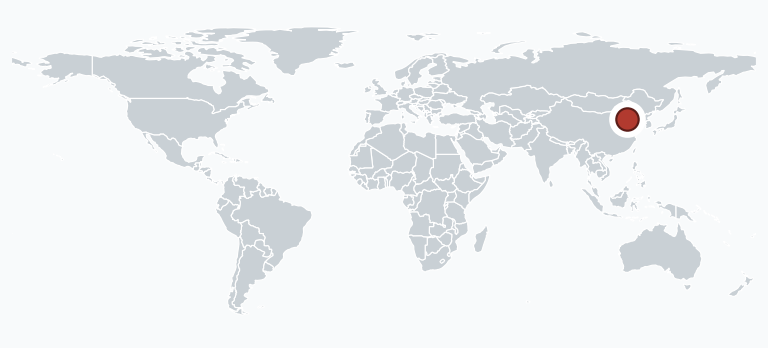
\includegraphics[width=\linewidth,keepaspectratio]{../figures/campus-locators/aifab-031-world-locator.png}
\par\smallskip
{\sffamily\scriptsize Coordinates: 38.979, 117.197.\par}
{\sffamily\scriptsize\color{black!68} Coordinates estimate the center of the four-road parcel described in the cited sources.\nobreak\textsuperscript{\href{\detokenize{https://www.sohu.com/a/581126452_121123526}}{\textcolor{accent}{1}}}\par}
\end{minipage}
\par\vspace{0.9em}
\noindent
\begin{minipage}[t]{\textwidth}
\raggedright
% Image-left evidence-right profile row
\begin{minipage}[t]{0.64\textwidth}
\vspace{0pt}\raggedright
\includegraphics[width=\linewidth,height=0.42\textheight,keepaspectratio,trim=0 0bp 0 0bp,clip]{../assets/campus-imagery/aifab-031.png}
\end{minipage}
\hfill
\begin{minipage}[t]{0.32\textwidth}
\vspace{0pt}\vspace{1.0em}\raggedright
{\sffamily\scriptsize World Imagery; source imagery dated May 16, 2025; source extract 0.634766 m grid; 2.6 km view. Source: Esri, Vantor, Earthstar Geographics, and the GIS User Community. Local imagery: Vantor Vivid Advanced (WV03), source dated 2025-05-16, Raster Basemaps 2026.R01. Map image is the intellectual property of Esri and is used herein under license. Copyright © 2026 Esri and its licensors. All rights reserved. Cropped and annotated by the authors.\nobreak\textsuperscript{\href{\detokenize{https://www.arcgis.com/home/item.html?id=10df2279f9684e4a9f6a7f08febac2a9}}{\textcolor{accent}{6}}} Yellow cross: cited location point.\par}
\medskip
{\footnotesize SMIC filings separately identify the Xiqing entity and support production capability, but the reviewed evidence does not establish current production at this campus.\nobreak\textsuperscript{\href{\detokenize{https://www1.hkexnews.hk/listedco/listconews/sehk/2026/0408/2026040801181.pdf}}{\textcolor{accent}{2}},\href{\detokenize{https://www1.hkexnews.hk/listedco/listconews/sehk/2022/0826/2022082601080.pdf}}{\textcolor{accent}{3}},\href{\detokenize{https://www1.hkexnews.hk/listedco/listconews/sehk/2026/0408/2026040802776_c.pdf}}{\textcolor{accent}{4}},\href{\detokenize{https://www.hkexnews.hk/listedco/listconews/sehk/2026/0326/2026032601650_c.pdf}}{\textcolor{accent}{5}}}\par}
\medskip
{\footnotesize\textbf{Documented wafer-fabrication capability:} Planned 28--180 nm line; the reviewed evidence supports capability but does not establish current production\nobreak\textsuperscript{\href{\detokenize{https://www1.hkexnews.hk/listedco/listconews/sehk/2022/0826/2022082601080.pdf}}{\textcolor{accent}{3}},\href{\detokenize{https://www1.hkexnews.hk/listedco/listconews/sehk/2026/0408/2026040802776_c.pdf}}{\textcolor{accent}{4}}}\par}
\end{minipage}
\end{minipage}
\par\vspace{0.65em}
\medskip
{\footnotesize\textbf{Named data-center AI accelerators or programs:} None identified in the sources reviewed.\par}
\smallskip
{\sffamily\scriptsize\color{black!62}\textbf{Other public catalogues (same campus; reviewed August 25, 2026):} \href{\detokenize{https://en.wikipedia.org/w/index.php?title=List_of_semiconductor_fabrication_plants&oldid=1370451124}\#\detokenize{Open_plants}}{Wikipedia fab list}.\par}
\medskip
{\sffamily\scriptsize\setlength{\emergencystretch}{1.5em}\textbf{Sources.} \textsuperscript{1}\,Site Selection 960 (republished by Sohu). \href{\detokenize{https://www.sohu.com/a/581126452_121123526}}{\enquote{Public report reproducing the four-road description for Tianjin land parcel G2022-03.}} August 30, 2022; \textsuperscript{2}\,SMIC. \href{\detokenize{https://www1.hkexnews.hk/listedco/listconews/sehk/2026/0408/2026040801181.pdf}}{\enquote{SMIC 2025 Annual Report.}} April 8, 2026; \textsuperscript{3}\,SMIC. \href{\detokenize{https://www1.hkexnews.hk/listedco/listconews/sehk/2022/0826/2022082601080.pdf}}{\enquote{Cooperation Framework Agreement for a Project in Tianjin.}} August 26, 2022; \textsuperscript{4}\,Semiconductor Manufacturing International Corporation. \href{\detokenize{https://www1.hkexnews.hk/listedco/listconews/sehk/2026/0408/2026040802776_c.pdf}}{\enquote{Response to Inquiry Concerning the Proposed Asset Purchase and Related Transaction.}} April 8, 2026; \textsuperscript{5}\,Semiconductor Manufacturing International Corporation. \href{\detokenize{https://www.hkexnews.hk/listedco/listconews/sehk/2026/0326/2026032601650_c.pdf}}{\enquote{Announcement on Expected 2026 Guarantee Limits for Subsidiaries.}} March 26, 2026; \textsuperscript{6}\,Esri. \href{\detokenize{https://www.arcgis.com/home/item.html?id=10df2279f9684e4a9f6a7f08febac2a9}}{\enquote{World Imagery.}} Accessed August 23, 2026.\par}
\vfill
\noindent{\color{hairline}\rule{\linewidth}{0.4pt}}\par\smallskip
{\sffamily\scriptsize\color{black!58} Evidence reviewed through August 25, 2026.\par}
\end{minipage}
\clearpage
% Campus profile AIFAB-021
\markright{Huali Fab 6}
\noindent\begin{minipage}[t][0.90\textheight][t]{\textwidth}
\noindent\begin{minipage}[t]{0.69\textwidth}
\raggedright
{\sffamily\bfseries\Large\color{accent} Huali Fab 6\par}
\smallskip
{\sffamily\small\textbf{Operator:} Hua Hong / Huali\quad \textbf{Location:} Shanghai, CHN\par}
{\sffamily\footnotesize\color{black!68}\textbf{Facility status:} Operating; a single source reports a 7 nm tapeout on Huali's line (as of 2026-08-10)\par}
\end{minipage}
\hfill
\begin{minipage}[t]{0.27\textwidth}
\raggedright
{\sffamily\bfseries\footnotesize World location}\par\smallskip
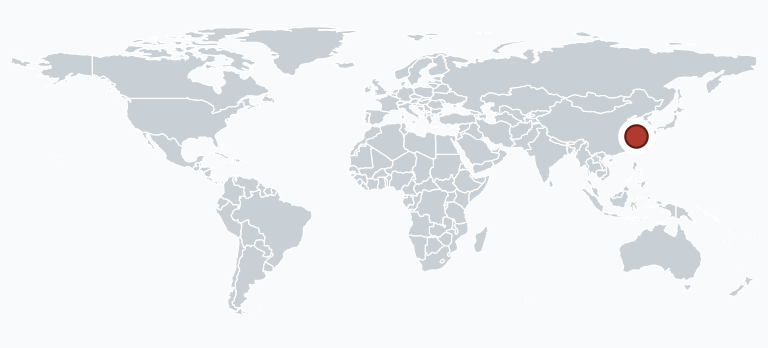
\includegraphics[width=\linewidth,keepaspectratio]{../figures/campus-locators/aifab-021-world-locator.png}
\par\smallskip
{\sffamily\scriptsize Coordinates: 31.077, 121.613.\par}
{\sffamily\scriptsize\color{black!68} Coordinates are the representative point returned for the cited OpenStreetMap feature.\nobreak\textsuperscript{\href{\detokenize{https://www.openstreetmap.org/way/1242527328}}{\textcolor{accent}{1}}}\par}
\end{minipage}
\par\vspace{0.9em}
\noindent
\begin{minipage}[t]{\textwidth}
\raggedright
% Image-left evidence-right profile row
\begin{minipage}[t]{0.64\textwidth}
\vspace{0pt}\raggedright
\includegraphics[width=\linewidth,height=0.42\textheight,keepaspectratio,trim=0 0bp 0 0bp,clip]{../assets/campus-imagery/aifab-021.png}
\end{minipage}
\hfill
\begin{minipage}[t]{0.32\textwidth}
\vspace{0pt}\vspace{1.0em}\raggedright
{\sffamily\scriptsize World Imagery; source imagery dates April 7, 2025 and April 9, 2025; source extract 0.488281 m grid; 2 km view. Source: Esri, Vantor, Earthstar Geographics, and the GIS User Community. Local imagery: Vantor Vivid Advanced (LG03), source dated 2025-04-07, Raster Basemaps 2025.R10; Vantor Vivid Advanced (LG03), source dated 2025-04-09, Raster Basemaps 2025.R10. Map image is the intellectual property of Esri and is used herein under license. Copyright © 2026 Esri and its licensors. All rights reserved. Cropped and annotated by the authors.\nobreak\textsuperscript{\href{\detokenize{https://www.arcgis.com/home/item.html?id=10df2279f9684e4a9f6a7f08febac2a9}}{\textcolor{accent}{4}}} Yellow cross: cited location point.\par}
\medskip
{\footnotesize Huali identifies Fab 6 as an operating manufacturing campus.\nobreak\textsuperscript{\href{\detokenize{https://www.hlmc.cn/aboutUs}}{\textcolor{accent}{2}},\href{\detokenize{https://www.investing.com/news/stock-market-news/exclusivechinas-no-2-chipmaker-readies-7-nm-production-as-beijing-ramps-up-selfsuffiency-drive-4561633}}{\textcolor{accent}{3}}}\par}
\medskip
{\footnotesize\textbf{Documented wafer-fabrication capability:} 28/22 nm production; independently reported 7 nm development\nobreak\textsuperscript{\href{\detokenize{https://www.investing.com/news/stock-market-news/exclusivechinas-no-2-chipmaker-readies-7-nm-production-as-beijing-ramps-up-selfsuffiency-drive-4561633}}{\textcolor{accent}{3}}}\par}
\end{minipage}
\end{minipage}
\par\vspace{0.65em}
\medskip
{\footnotesize\textbf{Named data-center AI accelerators or programs:}\par}
\begin{itemize}[leftmargin=1.25em,itemsep=0.35em,topsep=0.15em,parsep=0pt]
\item {\footnotesize\textbf{Biren --- unnamed 7 nm GPU tapeout design.} Reuters reports (one source) that Biren is using Huali's 7 nm line for tapeout and, separately, places Huali's 7 nm work at Fab 6.\nobreak\textsuperscript{\href{\detokenize{https://www.investing.com/news/stock-market-news/exclusivechinas-no-2-chipmaker-readies-7-nm-production-as-beijing-ramps-up-selfsuffiency-drive-4561633}}{\textcolor{accent}{3}}}\par {\scriptsize\color{black!62}\textbf{Limits of the evidence:} Reuters does not name the chip or its market, and this stage precedes mass production.\par}}
\end{itemize}
\smallskip
{\sffamily\scriptsize\color{black!62}\textbf{Other public catalogues (same campus; reviewed August 25, 2026):} \href{\detokenize{https://en.wikipedia.org/w/index.php?title=List_of_semiconductor_fabrication_plants&oldid=1370451124}\#\detokenize{Open_plants}}{Wikipedia fab list}.\par}
\medskip
{\sffamily\scriptsize\setlength{\emergencystretch}{1.5em}\textbf{Sources.} \textsuperscript{1}\,OpenStreetMap contributors. \href{\detokenize{https://www.openstreetmap.org/way/1242527328}}{\enquote{Huali Integrated Circuit mapped campus, OSM way 1242527328.}} Accessed August 11, 2026; \textsuperscript{2}\,Huali Microelectronics. \href{\detokenize{https://www.hlmc.cn/aboutUs}}{\enquote{Huali Microelectronics company overview.}} Accessed August 11, 2026; \textsuperscript{3}\,Reuters via Investing.com. \href{\detokenize{https://www.investing.com/news/stock-market-news/exclusivechinas-no-2-chipmaker-readies-7-nm-production-as-beijing-ramps-up-selfsuffiency-drive-4561633}}{\enquote{Exclusive-China's No. 2 chipmaker readies 7 nm production as Beijing ramps up self-sufficiency drive.}} March 16, 2026; \textsuperscript{4}\,Esri. \href{\detokenize{https://www.arcgis.com/home/item.html?id=10df2279f9684e4a9f6a7f08febac2a9}}{\enquote{World Imagery.}} Accessed August 23, 2026.\par}
\vfill
\noindent{\color{hairline}\rule{\linewidth}{0.4pt}}\par\smallskip
{\sffamily\scriptsize\color{black!58} Evidence reviewed through August 25, 2026.\par}
\end{minipage}
\clearpage
% Campus profile AIFAB-032
\markright{Wuxi Fab 7/Fab 9 campus}
\noindent\begin{minipage}[t][0.90\textheight][t]{\textwidth}
\noindent\begin{minipage}[t]{0.69\textwidth}
\raggedright
{\sffamily\bfseries\Large\color{accent} Wuxi Fab 7/Fab 9 campus\par}
\smallskip
{\sffamily\small\textbf{Operator:} Hua Hong Semiconductor\quad \textbf{Location:} Wuxi, Jiangsu, CHN\par}
{\sffamily\footnotesize\color{black!68}\textbf{Facility status:} Operating; production increasing (as of 2026-08-25)\par}
\end{minipage}
\hfill
\begin{minipage}[t]{0.27\textwidth}
\raggedright
{\sffamily\bfseries\footnotesize World location}\par\smallskip
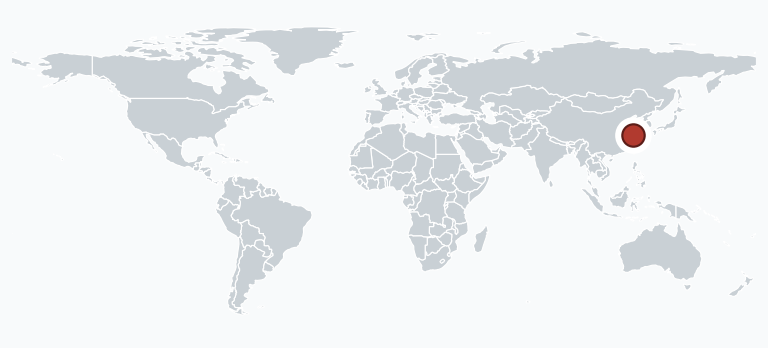
\includegraphics[width=\linewidth,keepaspectratio]{../figures/campus-locators/aifab-032-world-locator.png}
\par\smallskip
{\sffamily\scriptsize Coordinates: 31.524, 120.405.\par}
{\sffamily\scriptsize\color{black!68} Coordinates are the representative point returned for the cited OpenStreetMap feature.\nobreak\textsuperscript{\href{\detokenize{https://www.openstreetmap.org/way/843767291}}{\textcolor{accent}{1}}}\par}
\end{minipage}
\par\vspace{0.9em}
\noindent
\begin{minipage}[t]{\textwidth}
\raggedright
% Image-left evidence-right profile row
\begin{minipage}[t]{0.64\textwidth}
\vspace{0pt}\raggedright
\includegraphics[width=\linewidth,height=0.42\textheight,keepaspectratio,trim=0 0bp 0 0bp,clip]{../assets/campus-imagery/aifab-032.png}
\end{minipage}
\hfill
\begin{minipage}[t]{0.32\textwidth}
\vspace{0pt}\vspace{1.0em}\raggedright
{\sffamily\scriptsize World Imagery; source imagery dated April 3, 2025; source extract 0.585938 m grid; 2.4 km view. Source: Esri, Vantor, Earthstar Geographics, and the GIS User Community. Local imagery: Vantor Vivid Advanced (LG04), source dated 2025-04-03, Raster Basemaps 2025.R08. Map image is the intellectual property of Esri and is used herein under license. Copyright © 2026 Esri and its licensors. All rights reserved. Cropped and annotated by the authors.\nobreak\textsuperscript{\href{\detokenize{https://www.arcgis.com/home/item.html?id=10df2279f9684e4a9f6a7f08febac2a9}}{\textcolor{accent}{7}}} Yellow cross: cited location point.\par}
\medskip
{\footnotesize Government and regulatory records describe Fab 7 and Fab 9 as operating phases within one continuous Wuxi production base.\nobreak\textsuperscript{\href{\detokenize{https://www1.hkexnews.hk/listedco/listconews/sehk/2025/0408/2025040800831.pdf}}{\textcolor{accent}{2}},\href{\detokenize{https://www.wnd.gov.cn/doc/2024/08/26/4380012.shtml}}{\textcolor{accent}{3}},\href{\detokenize{https://www1.hkexnews.hk/listedco/listconews/sehk/2026/0813/2026081300401.pdf}}{\textcolor{accent}{4}},\href{\detokenize{https://www1.hkexnews.hk/listedco/listconews/sehk/2026/0409/2026040901618_c.pdf}}{\textcolor{accent}{5}},\href{\detokenize{https://www1.hkexnews.hk/listedco/listconews/sehk/2023/0224/2023022400027.pdf}}{\textcolor{accent}{6}}}\par}
\medskip
{\footnotesize\textbf{Documented wafer-fabrication capability:} One continuous campus containing operating Fab 7 and Fab 9; 90 nm through 65/55 nm specialty capability, with 40 nm also documented for Fab 9\nobreak\textsuperscript{\href{\detokenize{https://www1.hkexnews.hk/listedco/listconews/sehk/2025/0408/2025040800831.pdf}}{\textcolor{accent}{2}},\href{\detokenize{https://www.wnd.gov.cn/doc/2024/08/26/4380012.shtml}}{\textcolor{accent}{3}},\href{\detokenize{https://www1.hkexnews.hk/listedco/listconews/sehk/2026/0813/2026081300401.pdf}}{\textcolor{accent}{4}},\href{\detokenize{https://www1.hkexnews.hk/listedco/listconews/sehk/2026/0409/2026040901618_c.pdf}}{\textcolor{accent}{5}},\href{\detokenize{https://www1.hkexnews.hk/listedco/listconews/sehk/2023/0224/2023022400027.pdf}}{\textcolor{accent}{6}}}\par}
\end{minipage}
\end{minipage}
\par\vspace{0.65em}
\medskip
{\footnotesize\textbf{Named data-center AI accelerators or programs:} None identified in the sources reviewed.\par}
\smallskip
{\sffamily\scriptsize\color{black!62}\textbf{Other public catalogues (same campus; reviewed August 25, 2026):} \href{\detokenize{https://en.wikipedia.org/w/index.php?title=List_of_semiconductor_fabrication_plants&oldid=1370451124}\#\detokenize{Open_plants}}{Wikipedia fab list}.\par}
\medskip
{\sffamily\scriptsize\setlength{\emergencystretch}{1.5em}\textbf{Sources.} \textsuperscript{1}\,OpenStreetMap contributors. \href{\detokenize{https://www.openstreetmap.org/way/843767291}}{\enquote{Hua Hong Wuxi mapped industrial area, OSM way 843767291.}} Accessed August 25, 2026; \textsuperscript{2}\,Hua Hong Semiconductor. \href{\detokenize{https://www1.hkexnews.hk/listedco/listconews/sehk/2025/0408/2025040800831.pdf}}{\enquote{Hua Hong Semiconductor 2024 Annual Report.}} April 8, 2025; \textsuperscript{3}\,Wuxi Xinwu District People's Government. \href{\detokenize{https://www.wnd.gov.cn/doc/2024/08/26/4380012.shtml}}{\enquote{Quanguo shoupi! Ruxuan!}} [First national batch! Selected!] In Chinese. August 26, 2024; \textsuperscript{4}\,Hua Hong Grace Semiconductor (formerly Hua Hong Semiconductor). \href{\detokenize{https://www1.hkexnews.hk/listedco/listconews/sehk/2026/0813/2026081300401.pdf}}{\enquote{Reports 2026 Second Quarter Results.}} August 13, 2026; \textsuperscript{5}\,Hua Hong Semiconductor. \href{\detokenize{https://www1.hkexnews.hk/listedco/listconews/sehk/2026/0409/2026040901618_c.pdf}}{\enquote{Hua Hong Semiconductor 2025 Annual Report.}} April 9, 2026; \textsuperscript{6}\,Hua Hong Semiconductor. \href{\detokenize{https://www1.hkexnews.hk/listedco/listconews/sehk/2023/0224/2023022400027.pdf}}{\enquote{Major Transactions in Relation to the JV Agreement, the JV Investment Agreement and the Land Transfer Agreement.}} February 24, 2023; \textsuperscript{7}\,Esri. \href{\detokenize{https://www.arcgis.com/home/item.html?id=10df2279f9684e4a9f6a7f08febac2a9}}{\enquote{World Imagery.}} Accessed August 23, 2026.\par}
\vfill
\noindent{\color{hairline}\rule{\linewidth}{0.4pt}}\par\smallskip
{\sffamily\scriptsize\color{black!58} Evidence reviewed through August 25, 2026.\par}
\end{minipage}
\clearpage
% Campus profile AIFAB-006
\markright{Fab 8}
\noindent\begin{minipage}[t][0.90\textheight][t]{\textwidth}
\noindent\begin{minipage}[t]{0.69\textwidth}
\raggedright
{\sffamily\bfseries\Large\color{accent} Fab 8\par}
\smallskip
{\sffamily\small\textbf{Operator:} GlobalFoundries\quad \textbf{Location:} Malta, New York, USA\par}
{\sffamily\footnotesize\color{black!68}\textbf{Facility status:} Operating; expansion under construction (as of 2026-08-25)\par}
\end{minipage}
\hfill
\begin{minipage}[t]{0.27\textwidth}
\raggedright
{\sffamily\bfseries\footnotesize World location}\par\smallskip
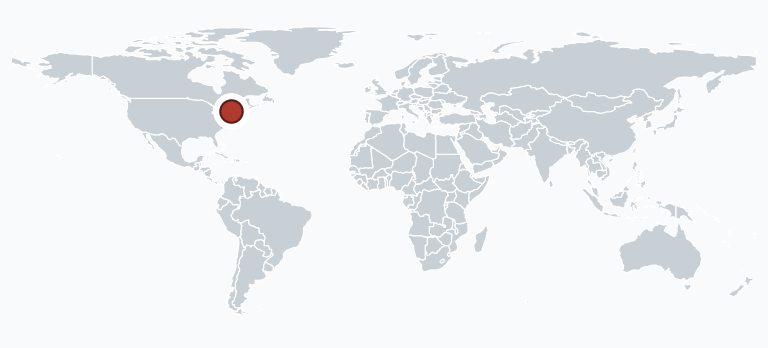
\includegraphics[width=\linewidth,keepaspectratio]{../figures/campus-locators/aifab-006-world-locator.png}
\par\smallskip
{\sffamily\scriptsize Coordinates: 42.970, -73.754.\par}
{\sffamily\scriptsize\color{black!68} Coordinates from a facility-center point in the cited U.S. EPA record.\nobreak\textsuperscript{\href{\detokenize{https://ofmpub.epa.gov/frs_public2/frs_rest_services.get_facilities?registry_id=110043863922&coordinates_output=yes&program_output=yes&output=JSON}}{\textcolor{accent}{1}}}\par}
\end{minipage}
\par\vspace{0.9em}
\noindent
\begin{minipage}[t]{\textwidth}
\raggedright
% Image-left evidence-right profile row
\begin{minipage}[t]{0.64\textwidth}
\vspace{0pt}\raggedright
\includegraphics[width=\linewidth,height=0.42\textheight,keepaspectratio,trim=0 0bp 0 0bp,clip]{../assets/campus-imagery/aifab-006.png}
\end{minipage}
\hfill
\begin{minipage}[t]{0.32\textwidth}
\vspace{0pt}\vspace{1.0em}\raggedright
{\sffamily\scriptsize New York State Office of Information Technology Services, New York State Digital Orthoimagery Program, Saratoga County 2024 one-foot four-band orthoimagery; exact flight date not stated; source extract 0.976562 m grid; 4 km view; cropped and annotated by the authors.\nobreak\textsuperscript{\href{\detokenize{https://data.ny.gov/Public-Safety/Statewide-Digital-Orthoimagery/amsv-rmfz}}{\textcolor{accent}{7}}} Yellow cross: cited location point.\par}
\medskip
{\footnotesize GlobalFoundries identifies Malta/Fab 8 as an operating manufacturing site with current production and an expansion under way.\nobreak\textsuperscript{\href{\detokenize{https://investors.gf.com/static-files/ef3116da-5334-46e0-9b6c-56d3e67b1b92}}{\textcolor{accent}{2}},\href{\detokenize{https://gf.com/news-and-events/news/globalfoundries-and-bae-systems-collaborate-on-semiconductors-for-space/}}{\textcolor{accent}{3}},\href{\detokenize{https://gf.com/news-and-events/blog/from-fab-to-the-field-accelerating-trusted-us-semiconductor-onshoring-for-mission-critical-defense/}}{\textcolor{accent}{4}}}\par}
\medskip
{\footnotesize\textbf{Documented wafer-fabrication capability:} 12LP (12 nm) FinFET and FDX/22FDX production; Fab 8 and related Malta capacity are expanding.\nobreak\textsuperscript{\href{\detokenize{https://investors.gf.com/static-files/ef3116da-5334-46e0-9b6c-56d3e67b1b92}}{\textcolor{accent}{2}},\href{\detokenize{https://gf.com/news-and-events/news/globalfoundries-and-bae-systems-collaborate-on-semiconductors-for-space/}}{\textcolor{accent}{3}},\href{\detokenize{https://gf.com/news-and-events/blog/from-fab-to-the-field-accelerating-trusted-us-semiconductor-onshoring-for-mission-critical-defense/}}{\textcolor{accent}{4}}}\par}
\end{minipage}
\end{minipage}
\par\vspace{0.65em}
\medskip
{\footnotesize\textbf{Named data-center AI accelerators or programs:}\par}
\begin{itemize}[leftmargin=1.25em,itemsep=0.35em,topsep=0.15em,parsep=0pt]
\item {\footnotesize\textbf{Enflame --- CloudBlazer T10.} GlobalFoundries scheduled CloudBlazer production at Fab 8 for early 2020, and Enflame later confirmed 12 nm production and commercial use.\nobreak\textsuperscript{\href{\detokenize{https://gf.com/news-and-events/news/globalfoundries-and-bae-systems-collaborate-on-semiconductors-for-space/}}{\textcolor{accent}{3}},\href{\detokenize{https://investors.gf.com/news-releases/news-release-details/enflame-technology-announces-cloudblazer-dtu-chip}}{\textcolor{accent}{5}},\href{\detokenize{https://www.yicai.com/news/101103178.html}}{\textcolor{accent}{6}}}\par {\scriptsize\color{black!62}\textbf{Limits of the evidence:} No reviewed source names the campus where that production took place.\par}}
\end{itemize}
\smallskip
{\sffamily\scriptsize\color{black!62}\textbf{Other public catalogues (same campus; reviewed August 25, 2026):} \href{\detokenize{https://en.wikipedia.org/w/index.php?title=List_of_semiconductor_fabrication_plants&oldid=1370451124}\#\detokenize{Open_plants}}{Wikipedia fab list}.\par}
\medskip
{\sffamily\scriptsize\setlength{\emergencystretch}{1.5em}\textbf{Sources.} \textsuperscript{1}\,U.S. Environmental Protection Agency. \href{\detokenize{https://ofmpub.epa.gov/frs_public2/frs_rest_services.get_facilities?registry_id=110043863922&coordinates_output=yes&program_output=yes&output=JSON}}{\enquote{Facility Registry Service record for GlobalFoundries Fab 8, registry 110043863922.}} Accessed August 25, 2026; \textsuperscript{2}\,GlobalFoundries. \href{\detokenize{https://investors.gf.com/static-files/ef3116da-5334-46e0-9b6c-56d3e67b1b92}}{\enquote{2025 Form 20-F.}} February 27, 2026; \textsuperscript{3}\,GlobalFoundries. \href{\detokenize{https://gf.com/news-and-events/news/globalfoundries-and-bae-systems-collaborate-on-semiconductors-for-space/}}{\enquote{GlobalFoundries and BAE Systems collaborate on semiconductors for space.}} November 19, 2025; \textsuperscript{4}\,GlobalFoundries. \href{\detokenize{https://gf.com/news-and-events/blog/from-fab-to-the-field-accelerating-trusted-us-semiconductor-onshoring-for-mission-critical-defense/}}{\enquote{From Fab to the Field: Accelerating Trusted U.S. Semiconductor Onshoring for Mission-Critical Defense.}} March 6, 2026; \textsuperscript{5}\,GlobalFoundries. \href{\detokenize{https://investors.gf.com/news-releases/news-release-details/enflame-technology-announces-cloudblazer-dtu-chip}}{\enquote{Enflame Technology Announces CloudBlazer with DTU Chip on GLOBALFOUNDRIES 12LP FinFET Platform for Data Center Training.}} December 12, 2019; \textsuperscript{6}\,Yicai. \href{\detokenize{https://www.yicai.com/news/101103178.html}}{\enquote{[Enflame Technology releases second-generation AI chip, volume production by year-end].}} In Chinese. July 7, 2021; \textsuperscript{7}\,New York State Office of Information Technology Services, Geospatial Services. \href{\detokenize{https://data.ny.gov/Public-Safety/Statewide-Digital-Orthoimagery/amsv-rmfz}}{\enquote{New York State Digital Orthoimagery Program: Saratoga County 2024.}} Accessed August 23, 2026.\par}
\vfill
\noindent{\color{hairline}\rule{\linewidth}{0.4pt}}\par\smallskip
{\sffamily\scriptsize\color{black!58} Evidence reviewed through August 25, 2026.\par}
\end{minipage}
\clearpage
% Campus profile AIFAB-013
\markright{Arizona / Ocotillo Campus}
\noindent\begin{minipage}[t][0.90\textheight][t]{\textwidth}
\noindent\begin{minipage}[t]{0.69\textwidth}
\raggedright
{\sffamily\bfseries\Large\color{accent} Arizona / Ocotillo Campus\par}
\smallskip
{\sffamily\small\textbf{Operator:} Intel\quad \textbf{Location:} Chandler, Arizona, USA\par}
{\sffamily\footnotesize\color{black!68}\textbf{Facility status:} Operating; expansion under construction (as of 2026-08-25)\par}
\end{minipage}
\hfill
\begin{minipage}[t]{0.27\textwidth}
\raggedright
{\sffamily\bfseries\footnotesize World location}\par\smallskip
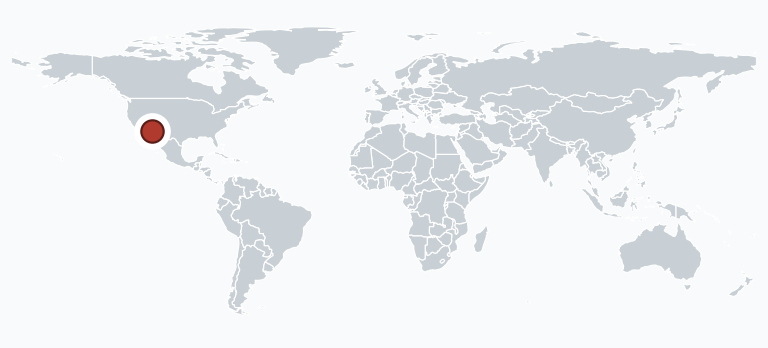
\includegraphics[width=\linewidth,keepaspectratio]{../figures/campus-locators/aifab-013-world-locator.png}
\par\smallskip
{\sffamily\scriptsize Coordinates: 33.246, -111.881.\par}
{\sffamily\scriptsize\color{black!68} Coordinates from a cited U.S. EPA address-matched point on the road at the campus edge.\nobreak\textsuperscript{\href{\detokenize{https://ofmpub.epa.gov/frs_public2/frs_rest_services.get_facilities?registry_id=110000471365&coordinates_output=yes&program_output=yes&output=JSON}}{\textcolor{accent}{1}}}\par}
\end{minipage}
\par\vspace{0.9em}
\noindent
\begin{minipage}[t]{\textwidth}
\raggedright
% Image-left evidence-right profile row
\begin{minipage}[t]{0.64\textwidth}
\vspace{0pt}\raggedright
\includegraphics[width=\linewidth,height=0.42\textheight,keepaspectratio,trim=0 0bp 0 0bp,clip]{../assets/campus-imagery/aifab-013.png}
\end{minipage}
\hfill
\begin{minipage}[t]{0.32\textwidth}
\vspace{0pt}\vspace{1.0em}\raggedright
{\sffamily\scriptsize Image: U.S. Department of Agriculture, National Agriculture Imagery Program (public domain); photographed September 15, 2023; source extract 1 m grid; 4 km view.\nobreak\textsuperscript{\href{\detokenize{https://planetarycomputer.microsoft.com/dataset/naip}}{\textcolor{accent}{11}}} Yellow cross: cited location point.\par}
\medskip
{\footnotesize Intel identifies Intel 7 and Intel 18A high-volume manufacturing at Ocotillo; Fab 52 is operating while Fab 62 and other expansion work continue.\nobreak\textsuperscript{\href{\detokenize{https://www.intc.com/filings-reports/all-sec-filings/content/0000050863-26-000011/intc-20251227.htm}}{\textcolor{accent}{2}},\href{\detokenize{https://web.archive.org/web/20260730143304/https://newsroom.intel.com/client-computing/intel-unveils-panther-lake-architecture-first-ai-pc-platform-built-on-18a}}{\textcolor{accent}{3}},\href{\detokenize{https://www.intc.com/filings-reports/all-sec-filings/content/0000050863-26-000061/proxy2026.htm}}{\textcolor{accent}{4}},\href{\detokenize{https://www.nist.gov/chips/intel-corporation-arizona-chandler}}{\textcolor{accent}{5}},\href{\detokenize{https://www.tomshardware.com/tech-industry/semiconductors/intels-fab-roadmap-examined}}{\textcolor{accent}{6}}}\par}
\medskip
{\footnotesize\textbf{Documented wafer-fabrication capability:} Intel 7 and Intel 18A high-volume manufacturing; Fab 52 is operational and Fab 62 and campus modernization remain expansion work.\nobreak\textsuperscript{\href{\detokenize{https://www.intc.com/filings-reports/all-sec-filings/content/0000050863-26-000011/intc-20251227.htm}}{\textcolor{accent}{2}},\href{\detokenize{https://web.archive.org/web/20260730143304/https://newsroom.intel.com/client-computing/intel-unveils-panther-lake-architecture-first-ai-pc-platform-built-on-18a}}{\textcolor{accent}{3}},\href{\detokenize{https://www.intc.com/filings-reports/all-sec-filings/content/0000050863-26-000061/proxy2026.htm}}{\textcolor{accent}{4}},\href{\detokenize{https://www.nist.gov/chips/intel-corporation-arizona-chandler}}{\textcolor{accent}{5}},\href{\detokenize{https://www.tomshardware.com/tech-industry/semiconductors/intels-fab-roadmap-examined}}{\textcolor{accent}{6}}}\par}
\end{minipage}
\end{minipage}
\par\vspace{0.65em}
\medskip
{\footnotesize\textbf{Named data-center AI accelerators or programs:}\par}
\begin{itemize}[leftmargin=1.25em,itemsep=0.35em,topsep=0.15em,parsep=0pt]
\item {\footnotesize\textbf{Positron --- Archer accelerator in Atlas system.} EE Times reports that Positron's Atlas system is built on Altera Agilex-7M FPGAs made by Intel in Chandler, Arizona; Business Insider also places Positron's chips in Chandler.\nobreak\textsuperscript{\href{\detokenize{https://web.archive.org/web/20260730143304/https://newsroom.intel.com/client-computing/intel-unveils-panther-lake-architecture-first-ai-pc-platform-built-on-18a}}{\textcolor{accent}{3}},\href{\detokenize{https://www.eetimes.com/startup-positron-takes-on-nvidia-with-fpgas/}}{\textcolor{accent}{7}},\href{\detokenize{https://finance.yahoo.com/news/pros-cons-making-advanced-chips-100002647.html}}{\textcolor{accent}{8}},\href{\detokenize{https://www.eetimes.com/positron-230-million-funding-led-by-financial-trading-firms/}}{\textcolor{accent}{9}},\href{\detokenize{https://www.positron.ai/atlas}}{\textcolor{accent}{10}}}\par {\scriptsize\color{black!62}\textbf{Limits of the evidence:} The campus is inferred: Intel's high-volume Chandler fabs are on Ocotillo. Intel and Altera do not name the fab or give a node or share. The chip is Altera's general-purpose FPGA, not a Positron design.\par}}
\end{itemize}
\smallskip
{\sffamily\scriptsize\color{black!62}\textbf{Other public catalogues (same campus; reviewed August 25, 2026):} \href{\detokenize{https://en.wikipedia.org/w/index.php?title=List_of_semiconductor_fabrication_plants&oldid=1370451124}\#\detokenize{Open_plants}}{Wikipedia fab list}; \href{\detokenize{https://www.wikidata.org/w/index.php?title=Q113325080&oldid=1694257473}}{Wikidata}.\par}
\medskip
{\sffamily\scriptsize\setlength{\emergencystretch}{1.5em}\textbf{Sources.} \textsuperscript{1}\,U.S. Environmental Protection Agency. \href{\detokenize{https://ofmpub.epa.gov/frs_public2/frs_rest_services.get_facilities?registry_id=110000471365&coordinates_output=yes&program_output=yes&output=JSON}}{\enquote{Facility Registry Service record for Intel Ocotillo, registry 110000471365.}} Accessed August 25, 2026; \textsuperscript{2}\,Intel. \href{\detokenize{https://www.intc.com/filings-reports/all-sec-filings/content/0000050863-26-000011/intc-20251227.htm}}{\enquote{Intel 2025 annual report on Form 10-K.}} 2026; \textsuperscript{3}\,Intel. \href{\detokenize{https://web.archive.org/web/20260730143304/https://newsroom.intel.com/client-computing/intel-unveils-panther-lake-architecture-first-ai-pc-platform-built-on-18a}}{\enquote{Intel Unveils Panther Lake Architecture: First AI PC Platform Built on 18A.}} October 9, 2025; \textsuperscript{4}\,Intel. \href{\detokenize{https://www.intc.com/filings-reports/all-sec-filings/content/0000050863-26-000061/proxy2026.htm}}{\enquote{2026 Proxy Statement.}} 2026; \textsuperscript{5}\,National Institute of Standards and Technology. \href{\detokenize{https://www.nist.gov/chips/intel-corporation-arizona-chandler}}{\enquote{Intel Corporation (Arizona).}} November 26, 2024; \textsuperscript{6}\,Tom's Hardware. \href{\detokenize{https://www.tomshardware.com/tech-industry/semiconductors/intels-fab-roadmap-examined}}{\enquote{Intel's fab roadmap examined --- Arizona, Ohio, Ireland, and the two deadlines deciding 14A process node.}} June 17, 2026; \textsuperscript{7}\,EE Times. \href{\detokenize{https://www.eetimes.com/startup-positron-takes-on-nvidia-with-fpgas/}}{\enquote{Startup Positron Takes On Nvidia With FPGAs.}} February 17, 2025; \textsuperscript{8}\,Business Insider via Yahoo Finance. \href{\detokenize{https://finance.yahoo.com/news/pros-cons-making-advanced-chips-100002647.html}}{\enquote{The pros and cons of making advanced chips in America.}} January 8, 2025; \textsuperscript{9}\,EE Times. \href{\detokenize{https://www.eetimes.com/positron-230-million-funding-led-by-financial-trading-firms/}}{\enquote{Positron's \$230M Funding Led By Financial Trading Firms.}} February 4, 2026; \textsuperscript{10}\,Positron AI. \href{\detokenize{https://www.positron.ai/atlas}}{\enquote{Positron Atlas inference system.}} Accessed August 11, 2026; \textsuperscript{11}\,U.S. Department of Agriculture. \href{\detokenize{https://planetarycomputer.microsoft.com/dataset/naip}}{\enquote{National Agriculture Imagery Program.}} Accessed August 23, 2026.\par}
\vfill
\noindent{\color{hairline}\rule{\linewidth}{0.4pt}}\par\smallskip
{\sffamily\scriptsize\color{black!58} Evidence reviewed through August 25, 2026.\par}
\end{minipage}
\clearpage
% Campus profile AIFAB-014
\markright{Oregon / Gordon Moore Park}
\noindent\begin{minipage}[t][0.90\textheight][t]{\textwidth}
\noindent\begin{minipage}[t]{0.69\textwidth}
\raggedright
{\sffamily\bfseries\Large\color{accent} Oregon / Gordon Moore Park\par}
\smallskip
{\sffamily\small\textbf{Operator:} Intel\quad \textbf{Location:} Hillsboro, Oregon, USA\par}
{\sffamily\footnotesize\color{black!68}\textbf{Facility status:} Operating (as of 2026-08-25)\par}
\end{minipage}
\hfill
\begin{minipage}[t]{0.27\textwidth}
\raggedright
{\sffamily\bfseries\footnotesize World location}\par\smallskip
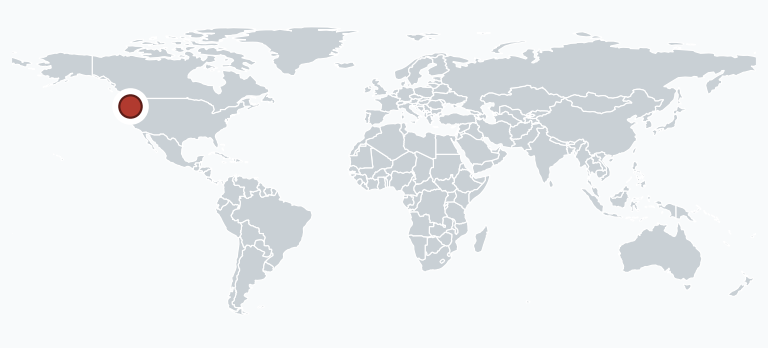
\includegraphics[width=\linewidth,keepaspectratio]{../figures/campus-locators/aifab-014-world-locator.png}
\par\smallskip
{\sffamily\scriptsize Coordinates: 45.543, -122.917.\par}
{\sffamily\scriptsize\color{black!68} Coordinates from a process-unit point in the cited U.S. EPA facility record.\nobreak\textsuperscript{\href{\detokenize{https://frs-public.epa.gov/ords/frs_public2/fii_query_dtl.disp_program_facility?p_registry_id=110000487018}}{\textcolor{accent}{1}}}\par}
\end{minipage}
\par\vspace{0.9em}
\noindent
\begin{minipage}[t]{\textwidth}
\raggedright
% Image-left evidence-right profile row
\begin{minipage}[t]{0.64\textwidth}
\vspace{0pt}\raggedright
\includegraphics[width=\linewidth,height=0.42\textheight,keepaspectratio,trim=0 0bp 0 0bp,clip]{../assets/campus-imagery/aifab-014.png}
\end{minipage}
\hfill
\begin{minipage}[t]{0.32\textwidth}
\vspace{0pt}\vspace{1.0em}\raggedright
{\sffamily\scriptsize State of Oregon, Oregon Statewide Imagery Program, 2024 statewide one-foot orthoimagery (acquisition and processing by Surdex, a Bowman company); photographed June-August 2024; source extract 0.976562 m grid; 4 km view; cropped and annotated by the authors.\nobreak\textsuperscript{\href{\detokenize{https://imagery.oregonexplorer.info/arcgis/rest/services/OSIP_2024/OSIP_2024_WM/ImageServer}}{\textcolor{accent}{5}}} Yellow cross: cited location point.\par}
\medskip
{\footnotesize Intel identifies Intel 18A high-volume manufacturing and next-node research and development at Gordon Moore Park.\nobreak\textsuperscript{\href{\detokenize{https://www.intc.com/filings-reports/all-sec-filings/content/0000050863-26-000011/intc-20251227.htm}}{\textcolor{accent}{2}},\href{\detokenize{https://www.intc.com/filings-reports/all-sec-filings/content/0000050863-26-000061/proxy2026.htm}}{\textcolor{accent}{3}},\href{\detokenize{https://web.archive.org/web/20260730143304/https://newsroom.intel.com/client-computing/intel-unveils-panther-lake-architecture-first-ai-pc-platform-built-on-18a}}{\textcolor{accent}{4}}}\par}
\medskip
{\footnotesize\textbf{Documented wafer-fabrication capability:} Intel 18A high-volume manufacturing and next-node research and development.\nobreak\textsuperscript{\href{\detokenize{https://www.intc.com/filings-reports/all-sec-filings/content/0000050863-26-000011/intc-20251227.htm}}{\textcolor{accent}{2}},\href{\detokenize{https://www.intc.com/filings-reports/all-sec-filings/content/0000050863-26-000061/proxy2026.htm}}{\textcolor{accent}{3}},\href{\detokenize{https://web.archive.org/web/20260730143304/https://newsroom.intel.com/client-computing/intel-unveils-panther-lake-architecture-first-ai-pc-platform-built-on-18a}}{\textcolor{accent}{4}}}\par}
\end{minipage}
\end{minipage}
\par\vspace{0.65em}
\medskip
{\footnotesize\textbf{Named data-center AI accelerators or programs:} None identified in the sources reviewed.\par}
\smallskip
{\sffamily\scriptsize\color{black!62}\textbf{Other public catalogues (same campus; reviewed August 25, 2026):} \href{\detokenize{https://en.wikipedia.org/w/index.php?title=List_of_semiconductor_fabrication_plants&oldid=1370451124}\#\detokenize{Open_plants}}{Wikipedia fab list}; \href{\detokenize{https://www.wikidata.org/w/index.php?title=Q113380692&oldid=1694236879}}{Wikidata}; \href{\detokenize{https://github.com/aminalav/chip-sense/blob/93d22afe9e1309a7bebd6c7c96541f069f1d67ac/src/data/fab-sites.json}\#\detokenize{L143-L150}}{Chip Sense}.\par}
\medskip
{\sffamily\scriptsize\setlength{\emergencystretch}{1.5em}\textbf{Sources.} \textsuperscript{1}\,U.S. Environmental Protection Agency. \href{\detokenize{https://frs-public.epa.gov/ords/frs_public2/fii_query_dtl.disp_program_facility?p_registry_id=110000487018}}{\enquote{Facility Registry Service record for Intel Gordon Moore Park, registry 110000487018.}} Accessed August 25, 2026; \textsuperscript{2}\,Intel. \href{\detokenize{https://www.intc.com/filings-reports/all-sec-filings/content/0000050863-26-000011/intc-20251227.htm}}{\enquote{Intel 2025 annual report on Form 10-K.}} 2026; \textsuperscript{3}\,Intel. \href{\detokenize{https://www.intc.com/filings-reports/all-sec-filings/content/0000050863-26-000061/proxy2026.htm}}{\enquote{2026 Proxy Statement.}} 2026; \textsuperscript{4}\,Intel. \href{\detokenize{https://web.archive.org/web/20260730143304/https://newsroom.intel.com/client-computing/intel-unveils-panther-lake-architecture-first-ai-pc-platform-built-on-18a}}{\enquote{Intel Unveils Panther Lake Architecture: First AI PC Platform Built on 18A.}} October 9, 2025; \textsuperscript{5}\,State of Oregon, Oregon Statewide Imagery Program (OSIP). \href{\detokenize{https://imagery.oregonexplorer.info/arcgis/rest/services/OSIP_2024/OSIP_2024_WM/ImageServer}}{\enquote{2024 Statewide One-Foot Orthoimagery.}} Accessed August 23, 2026.\par}
\vfill
\noindent{\color{hairline}\rule{\linewidth}{0.4pt}}\par\smallskip
{\sffamily\scriptsize\color{black!58} Evidence reviewed through August 25, 2026.\par}
\end{minipage}
\clearpage
% Campus profile AIFAB-027
\markright{Ohio One campus}
\noindent\begin{minipage}[t][0.90\textheight][t]{\textwidth}
\noindent\begin{minipage}[t]{0.69\textwidth}
\raggedright
{\sffamily\bfseries\Large\color{accent} Ohio One campus\par}
\smallskip
{\sffamily\small\textbf{Operator:} Intel\quad \textbf{Location:} New Albany, Ohio, USA\par}
{\sffamily\footnotesize\color{black!68}\textbf{Facility status:} Under construction; schedule delayed (as of 2026-08-25)\par}
\end{minipage}
\hfill
\begin{minipage}[t]{0.27\textwidth}
\raggedright
{\sffamily\bfseries\footnotesize World location}\par\smallskip
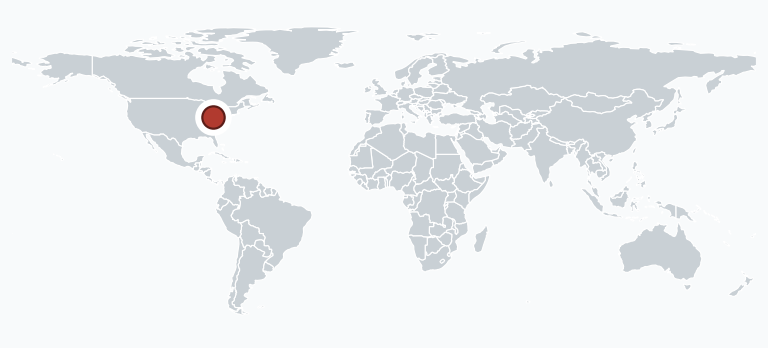
\includegraphics[width=\linewidth,keepaspectratio]{../figures/campus-locators/aifab-027-world-locator.png}
\par\smallskip
{\sffamily\scriptsize Coordinates: 40.117, -82.711.\par}
{\sffamily\scriptsize\color{black!68} Coordinates are the representative point returned for the cited OpenStreetMap feature.\nobreak\textsuperscript{\href{\detokenize{https://www.openstreetmap.org/way/1093263212}}{\textcolor{accent}{1}}}\par}
\end{minipage}
\par\vspace{0.9em}
\noindent
\begin{minipage}[t]{\textwidth}
\raggedright
% Image-left evidence-right profile row
\begin{minipage}[t]{0.64\textwidth}
\vspace{0pt}\raggedright
\includegraphics[width=\linewidth,height=0.42\textheight,keepaspectratio,trim=0 0bp 0 0bp,clip]{../assets/campus-imagery/aifab-027.png}
\end{minipage}
\hfill
\begin{minipage}[t]{0.32\textwidth}
\vspace{0pt}\vspace{1.0em}\raggedright
{\sffamily\scriptsize State of Ohio, Ohio Statewide Imagery Program, Most Current Imagery service; 2025 three-inch imagery over the campus with 2023 peripheral edge fill; source extract 0.976562 m grid; 4 km view; cropped and annotated by the authors.\nobreak\textsuperscript{\href{\detokenize{https://maps.ohio.gov/image/rest/services/osip_most_current/ImageServer}}{\textcolor{accent}{8}}} Yellow cross: cited location point.\par}
\medskip
{\footnotesize Intel identifies this as a leading-edge campus with two fab modules under construction. It set 2030--2032 module dates in February 2025, then slowed work further. The Columbus Dispatch reported that Intel gave a firmer timeline in a 2026 state report; June 2026 reporting still listed 2030--2032 operations.\nobreak\textsuperscript{\href{\detokenize{https://web.archive.org/web/20260824065634/https://newsroom.intel.com/corporate/ohio-one-construction-timeline-update}}{\textcolor{accent}{2}},\href{\detokenize{https://web.archive.org/web/20260711062821/https://newsroom.intel.com/corporate/lip-bu-tan-steps-in-the-right-direction}}{\textcolor{accent}{3}},\href{\detokenize{https://www.intc.com/filings-reports/all-sec-filings/content/0000050863-26-000157/intc-20260627.htm}}{\textcolor{accent}{4}},\href{\detokenize{https://www.dispatch.com/story/business/information-technology/2026/03/02/intel-provides-firmer-completion-date-plans-for-ohio-one-project-chip-factory/88943609007/}}{\textcolor{accent}{5}},\href{\detokenize{https://www.tomshardware.com/tech-industry/semiconductors/intels-fab-roadmap-examined}}{\textcolor{accent}{6}},\href{\detokenize{https://www.nist.gov/chips/intel-corporation-ohio-new-albany}}{\textcolor{accent}{7}}}\par}
\medskip
{\footnotesize\textbf{Documented wafer-fabrication capability:} Two leading-edge fabs under slowed construction; the CHIPS award record lists Intel 14A and future nodes for the campus.\nobreak\textsuperscript{\href{\detokenize{https://web.archive.org/web/20260824065634/https://newsroom.intel.com/corporate/ohio-one-construction-timeline-update}}{\textcolor{accent}{2}},\href{\detokenize{https://web.archive.org/web/20260711062821/https://newsroom.intel.com/corporate/lip-bu-tan-steps-in-the-right-direction}}{\textcolor{accent}{3}},\href{\detokenize{https://www.intc.com/filings-reports/all-sec-filings/content/0000050863-26-000157/intc-20260627.htm}}{\textcolor{accent}{4}},\href{\detokenize{https://www.nist.gov/chips/intel-corporation-ohio-new-albany}}{\textcolor{accent}{7}}}\par}
\end{minipage}
\end{minipage}
\par\vspace{0.65em}
\medskip
{\footnotesize\textbf{Named data-center AI accelerators or programs:} None identified in the sources reviewed.\par}
\medskip
{\sffamily\scriptsize\setlength{\emergencystretch}{1.5em}\textbf{Sources.} \textsuperscript{1}\,OpenStreetMap contributors. \href{\detokenize{https://www.openstreetmap.org/way/1093263212}}{\enquote{Intel Ohio One mapped construction area, OSM way 1093263212.}} Accessed August 11, 2026; \textsuperscript{2}\,Intel. \href{\detokenize{https://web.archive.org/web/20260824065634/https://newsroom.intel.com/corporate/ohio-one-construction-timeline-update}}{\enquote{Ohio One Construction Timeline Update.}} February 28, 2025; \textsuperscript{3}\,Intel. \href{\detokenize{https://web.archive.org/web/20260711062821/https://newsroom.intel.com/corporate/lip-bu-tan-steps-in-the-right-direction}}{\enquote{Lip-Bu Tan: Steps in the Right Direction.}} July 24, 2025; \textsuperscript{4}\,Intel Corporation. \href{\detokenize{https://www.intc.com/filings-reports/all-sec-filings/content/0000050863-26-000157/intc-20260627.htm}}{\enquote{Quarterly Report for the quarter ended June 27, 2026.}} July 24, 2026; \textsuperscript{5}\,The Columbus Dispatch. \href{\detokenize{https://www.dispatch.com/story/business/information-technology/2026/03/02/intel-provides-firmer-completion-date-plans-for-ohio-one-project-chip-factory/88943609007/}}{\enquote{Intel provides firmer completion date plans for `Ohio One' project.}} March 2, 2026; \textsuperscript{6}\,Tom's Hardware. \href{\detokenize{https://www.tomshardware.com/tech-industry/semiconductors/intels-fab-roadmap-examined}}{\enquote{Intel's fab roadmap examined --- Arizona, Ohio, Ireland, and the two deadlines deciding 14A process node.}} June 17, 2026; \textsuperscript{7}\,National Institute of Standards and Technology. \href{\detokenize{https://www.nist.gov/chips/intel-corporation-ohio-new-albany}}{\enquote{Intel Corporation (Ohio).}} November 26, 2024; \textsuperscript{8}\,State of Ohio, Ohio Statewide Imagery Program. \href{\detokenize{https://maps.ohio.gov/image/rest/services/osip_most_current/ImageServer}}{\enquote{Ohio OSIP Most Current Imagery.}} Accessed August 23, 2026.\par}
\vfill
\noindent{\color{hairline}\rule{\linewidth}{0.4pt}}\par\smallskip
{\sffamily\scriptsize\color{black!58} Evidence reviewed through August 25, 2026.\par}
\end{minipage}
\clearpage
% Campus profile AIFAB-011
\markright{Austin Campus}
\noindent\begin{minipage}[t][0.90\textheight][t]{\textwidth}
\noindent\begin{minipage}[t]{0.69\textwidth}
\raggedright
{\sffamily\bfseries\Large\color{accent} Austin Campus\par}
\smallskip
{\sffamily\small\textbf{Operator:} Samsung Electronics\quad \textbf{Location:} Austin, Texas, USA\par}
{\sffamily\footnotesize\color{black!68}\textbf{Facility status:} Operating (as of 2026-08-25)\par}
\end{minipage}
\hfill
\begin{minipage}[t]{0.27\textwidth}
\raggedright
{\sffamily\bfseries\footnotesize World location}\par\smallskip
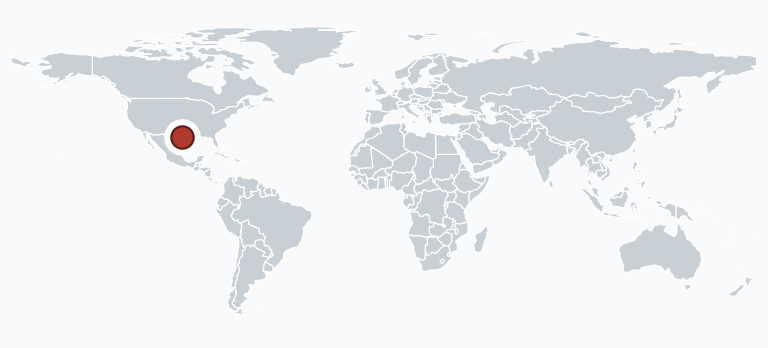
\includegraphics[width=\linewidth,keepaspectratio]{../figures/campus-locators/aifab-011-world-locator.png}
\par\smallskip
{\sffamily\scriptsize Coordinates: 30.375, -97.631.\par}
{\sffamily\scriptsize\color{black!68} Coordinates from an air-stack point in the cited U.S. EPA facility record.\nobreak\textsuperscript{\href{\detokenize{https://ofmpub.epa.gov/frs_public2/frs_rest_services.get_facilities?registry_id=110000465531&coordinates_output=yes&program_output=yes&output=JSON}}{\textcolor{accent}{1}}}\par}
\end{minipage}
\par\vspace{0.9em}
\noindent
\begin{minipage}[t]{\textwidth}
\raggedright
% Image-left evidence-right profile row
\begin{minipage}[t]{0.64\textwidth}
\vspace{0pt}\raggedright
\includegraphics[width=\linewidth,height=0.42\textheight,keepaspectratio,trim=0 0bp 0 0bp,clip]{../assets/campus-imagery/aifab-011.png}
\end{minipage}
\hfill
\begin{minipage}[t]{0.32\textwidth}
\vspace{0pt}\vspace{1.0em}\raggedright
{\sffamily\scriptsize Capital Area Council of Governments, CAPCOG Imagery 2022 (acquired by Surdex; distributed by the Texas Geographic Information Office under CC0 1.0; tiles via OpenStreetMap US Imagery); photographed January 4 and 22, 2022; source extract 1.0304 m grid; 4 km view.\nobreak\textsuperscript{\href{\detokenize{https://api.tnris.org/api/v1/collections/a15f67db-9535-464e-9058-f447325b6251}}{\textcolor{accent}{3}}} Yellow cross: cited location point.\par}
\medskip
{\footnotesize Samsung identifies Austin as an operating campus with processes from 65 nm through 14 nm.\nobreak\textsuperscript{\href{\detokenize{https://semiconductor.samsung.com/foundry/manufacturing/manufacturing-sites/}}{\textcolor{accent}{2}}}\par}
\medskip
{\footnotesize\textbf{Documented wafer-fabrication capability:} 65 nm through 14 nm\nobreak\textsuperscript{\href{\detokenize{https://semiconductor.samsung.com/foundry/manufacturing/manufacturing-sites/}}{\textcolor{accent}{2}}}\par}
\end{minipage}
\end{minipage}
\par\vspace{0.65em}
\medskip
{\footnotesize\textbf{Named data-center AI accelerators or programs:} None identified in the sources reviewed.\par}
\smallskip
{\sffamily\scriptsize\color{black!62}\textbf{Other public catalogues (same campus; reviewed August 25, 2026):} \href{\detokenize{https://en.wikipedia.org/w/index.php?title=List_of_semiconductor_fabrication_plants&oldid=1370451124}\#\detokenize{Open_plants}}{Wikipedia fab list}; \href{\detokenize{https://github.com/aminalav/chip-sense/blob/93d22afe9e1309a7bebd6c7c96541f069f1d67ac/src/data/fab-sites.json}\#\detokenize{L53-L60}}{Chip Sense}.\par}
\medskip
{\sffamily\scriptsize\setlength{\emergencystretch}{1.5em}\textbf{Sources.} \textsuperscript{1}\,U.S. Environmental Protection Agency. \href{\detokenize{https://ofmpub.epa.gov/frs_public2/frs_rest_services.get_facilities?registry_id=110000465531&coordinates_output=yes&program_output=yes&output=JSON}}{\enquote{Facility Registry Service record for Samsung Austin, registry 110000465531.}} Accessed August 25, 2026; \textsuperscript{2}\,Samsung Electronics. \href{\detokenize{https://semiconductor.samsung.com/foundry/manufacturing/manufacturing-sites/}}{\enquote{Samsung Foundry manufacturing sites.}} Accessed August 11, 2026; \textsuperscript{3}\,Capital Area Council of Governments and Texas Geographic Information Office. \href{\detokenize{https://api.tnris.org/api/v1/collections/a15f67db-9535-464e-9058-f447325b6251}}{\enquote{CAPCOG Imagery 2022.}} Accessed August 23, 2026.\par}
\vfill
\noindent{\color{hairline}\rule{\linewidth}{0.4pt}}\par\smallskip
{\sffamily\scriptsize\color{black!58} Evidence reviewed through August 25, 2026.\par}
\end{minipage}
\clearpage
% Campus profile AIFAB-019
\markright{Taylor Campus}
\noindent\begin{minipage}[t][0.90\textheight][t]{\textwidth}
\noindent\begin{minipage}[t]{0.69\textwidth}
\raggedright
{\sffamily\bfseries\Large\color{accent} Taylor Campus\par}
\smallskip
{\sffamily\small\textbf{Operator:} Samsung Electronics\quad \textbf{Location:} Taylor, Texas, USA\par}
{\sffamily\footnotesize\color{black!68}\textbf{Facility status:} Under construction; pre-operational (as of 2026-08-25)\par}
\end{minipage}
\hfill
\begin{minipage}[t]{0.27\textwidth}
\raggedright
{\sffamily\bfseries\footnotesize World location}\par\smallskip
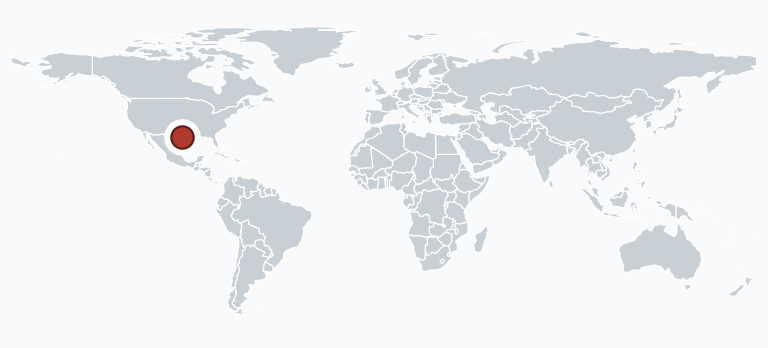
\includegraphics[width=\linewidth,keepaspectratio]{../figures/campus-locators/aifab-019-world-locator.png}
\par\smallskip
{\sffamily\scriptsize Coordinates: 30.537, -97.453.\par}
{\sffamily\scriptsize\color{black!68} Coordinates are the representative point returned for the cited OpenStreetMap feature.\nobreak\textsuperscript{\href{\detokenize{https://www.openstreetmap.org/way/1454508020}}{\textcolor{accent}{1}}}\par}
\end{minipage}
\par\vspace{0.9em}
\noindent
\begin{minipage}[t]{\textwidth}
\raggedright
% Image-left evidence-right profile row
\begin{minipage}[t]{0.64\textwidth}
\vspace{0pt}\raggedright
\includegraphics[width=\linewidth,height=0.42\textheight,keepaspectratio,trim=0 0bp 0 0bp,clip]{../assets/campus-imagery/aifab-019.png}
\end{minipage}
\hfill
\begin{minipage}[t]{0.32\textwidth}
\vspace{0pt}\vspace{1.0em}\raggedright
{\sffamily\scriptsize World Imagery; source imagery dated October 15, 2025; source extract 0.78125 m grid; 3.2 km view. Source: Esri, Vantor, Earthstar Geographics, and the GIS User Community. Local imagery: Williamson County TX Williamson County2025 (Williamson County Orthos), source dated 2025-10-15, Raster Basemaps 2026.R03. Map image is the intellectual property of Esri and is used herein under license. Copyright © 2026 Esri and its licensors. All rights reserved. Cropped and annotated by the authors.\nobreak\textsuperscript{\href{\detokenize{https://www.arcgis.com/home/item.html?id=10df2279f9684e4a9f6a7f08febac2a9}}{\textcolor{accent}{10}}} Yellow cross: cited location point.\par}
\medskip
{\footnotesize Samsung describes Taylor Fab 1 as preparing to begin operations in 2026, with 2 nm mass production targeted for 2027; Fab 2 is a later construction phase.\nobreak\textsuperscript{\href{\detokenize{https://semiconductor.samsung.com/sas/company/taylor/}}{\textcolor{accent}{2}},\href{\detokenize{https://irsvc.teletogether.com/sec/pdf/2026Q1_script_eng.pdf?1=}}{\textcolor{accent}{3}},\href{\detokenize{https://irsvc.teletogether.com/sec/pdf/2026Q2_script_eng.pdf?1=}}{\textcolor{accent}{4}},\href{\detokenize{https://image.semiconductor.samsung.com/content/samsung/p6/semiconductor-us/sas/chips-and-science-act_240416/samsung-factsheet-chips-final.pdf}}{\textcolor{accent}{5}}}\par}
\medskip
{\footnotesize\textbf{Documented wafer-fabrication capability:} Fab 1 planned for 2 nm\nobreak\textsuperscript{\href{\detokenize{https://irsvc.teletogether.com/sec/pdf/2026Q1_script_eng.pdf?1=}}{\textcolor{accent}{3}},\href{\detokenize{https://irsvc.teletogether.com/sec/pdf/2026Q2_script_eng.pdf?1=}}{\textcolor{accent}{4}},\href{\detokenize{https://image.semiconductor.samsung.com/content/samsung/p6/semiconductor-us/sas/chips-and-science-act_240416/samsung-factsheet-chips-final.pdf}}{\textcolor{accent}{5}}}\par}
\end{minipage}
\end{minipage}
\par\vspace{0.65em}
\medskip
{\footnotesize\textbf{Named data-center AI accelerators or programs:}\par}
\begin{itemize}[leftmargin=1.25em,itemsep=0.35em,topsep=0.15em,parsep=0pt]
\item {\footnotesize\textbf{Tesla --- AI6.} Tesla's CEO said in January 2026 that AI6 is for Optimus and data centers and in April 2026 that it would use Samsung's 2 nm fab in Texas.\nobreak\textsuperscript{\href{\detokenize{https://irsvc.teletogether.com/sec/pdf/2026Q2_script_eng.pdf?1=}}{\textcolor{accent}{4}},\href{\detokenize{https://www.koreajoongangdaily.com/business/musk-confirms-samsung-tsmc-to-produce-future-ai6-chips/12606378}}{\textcolor{accent}{6}},\href{\detokenize{https://electrek.co/2026/07/13/samsung-taylor-fab-tesla-ai5-chip-2nm/}}{\textcolor{accent}{7}},\href{\detokenize{https://www.notateslaapp.com/news/3515/musk-targets-9-month-chip-cycle-for-tesla-talks-ai5-ai6-and-space-based-ai}}{\textcolor{accent}{8}}}\par {\scriptsize\color{black!62}\textbf{Limits of the evidence:} A plan: a July 2026 report put mass production no earlier than late 2027.\par}}
\item {\footnotesize\textbf{Tesla --- AI5.} In October 2025, Tesla's CEO said Samsung would make AI5 in Texas; in July 2026, a Samsung Foundry engineer's post placed it at Taylor on 2 nm.\nobreak\textsuperscript{\href{\detokenize{https://irsvc.teletogether.com/sec/pdf/2026Q2_script_eng.pdf?1=}}{\textcolor{accent}{4}},\href{\detokenize{https://electrek.co/2026/07/13/samsung-taylor-fab-tesla-ai5-chip-2nm/}}{\textcolor{accent}{7}},\href{\detokenize{https://www.cnbc.com/2025/10/22/elon-musk-tesla-ai5-nvidia.html}}{\textcolor{accent}{9}}}\par {\scriptsize\color{black!62}\textbf{Limits of the evidence:} A plan: the post was later deleted, and Musk has pointed to mass production by mid-2027.\par}}
\end{itemize}
\smallskip
{\sffamily\scriptsize\color{black!62}\textbf{Other public catalogues (same campus; reviewed August 25, 2026):} \href{\detokenize{https://en.wikipedia.org/w/index.php?title=List_of_semiconductor_fabrication_plants&oldid=1370451124}\#\detokenize{Open_plants}}{Wikipedia fab list}; \href{\detokenize{https://github.com/aminalav/chip-sense/blob/93d22afe9e1309a7bebd6c7c96541f069f1d67ac/src/data/fab-sites.json}\#\detokenize{L43-L50}}{Chip Sense}.\par}
\medskip
{\sffamily\scriptsize\setlength{\emergencystretch}{1.5em}\textbf{Sources.} \textsuperscript{1}\,OpenStreetMap contributors. \href{\detokenize{https://www.openstreetmap.org/way/1454508020}}{\enquote{Samsung Taylor Fab 1 mapped building, OSM way 1454508020.}} Accessed August 11, 2026; \textsuperscript{2}\,Samsung Electronics. \href{\detokenize{https://semiconductor.samsung.com/sas/company/taylor/}}{\enquote{Samsung Austin Semiconductor Taylor site.}} Accessed August 11, 2026; \textsuperscript{3}\,Samsung Electronics. \href{\detokenize{https://irsvc.teletogether.com/sec/pdf/2026Q1_script_eng.pdf?1=}}{\enquote{First quarter 2026 earnings conference call.}} April 30, 2026; \textsuperscript{4}\,Samsung Electronics. \href{\detokenize{https://irsvc.teletogether.com/sec/pdf/2026Q2_script_eng.pdf?1=}}{\enquote{Second quarter 2026 earnings conference call.}} July 30, 2026; \textsuperscript{5}\,Samsung Electronics. \href{\detokenize{https://image.semiconductor.samsung.com/content/samsung/p6/semiconductor-us/sas/chips-and-science-act_240416/samsung-factsheet-chips-final.pdf}}{\enquote{With CHIPS Award, Samsung Continues to Fuel American Innovation.}} April 15, 2024; \textsuperscript{6}\,Korea JoongAng Daily. \href{\detokenize{https://www.koreajoongangdaily.com/business/musk-confirms-samsung-tsmc-to-produce-future-ai6-chips/12606378}}{\enquote{Musk confirms Samsung, TSMC to produce future AI6 chips.}} April 16, 2026; \textsuperscript{7}\,Electrek. \href{\detokenize{https://electrek.co/2026/07/13/samsung-taylor-fab-tesla-ai5-chip-2nm/}}{\enquote{Samsung's Texas fab enters production for Tesla's AI5 chip on 2nm.}} July 13, 2026; \textsuperscript{8}\,Not a Tesla App. \href{\detokenize{https://www.notateslaapp.com/news/3515/musk-targets-9-month-chip-cycle-for-tesla-talks-ai5-ai6-and-space-based-ai}}{\enquote{Musk Targets 9-Month Chip Cycle for Tesla; Talks AI5, AI6 and Space-Based AI.}} January 19, 2026; \textsuperscript{9}\,CNBC. \href{\detokenize{https://www.cnbc.com/2025/10/22/elon-musk-tesla-ai5-nvidia.html}}{\enquote{Tesla `not about to replace Nvidia' as EV maker develops chips for cars, robots, Musk says.}} October 22, 2025; \textsuperscript{10}\,Esri. \href{\detokenize{https://www.arcgis.com/home/item.html?id=10df2279f9684e4a9f6a7f08febac2a9}}{\enquote{World Imagery.}} Accessed August 23, 2026.\par}
\vfill
\noindent{\color{hairline}\rule{\linewidth}{0.4pt}}\par\smallskip
{\sffamily\scriptsize\color{black!58} Evidence reviewed through August 25, 2026.\par}
\end{minipage}
\clearpage
% Campus profile AIFAB-003
\markright{Arizona campus / corporate Fab 21}
\noindent\begin{minipage}[t][0.90\textheight][t]{\textwidth}
\noindent\begin{minipage}[t]{0.69\textwidth}
\raggedright
{\sffamily\bfseries\Large\color{accent} Arizona campus / corporate Fab 21\par}
\smallskip
{\sffamily\small\textbf{Operator:} TSMC\quad \textbf{Location:} Phoenix, Arizona, USA\par}
{\sffamily\footnotesize\color{black!68}\textbf{Facility status:} Operating; expansion under construction (as of 2026-08-25)\par}
\end{minipage}
\hfill
\begin{minipage}[t]{0.27\textwidth}
\raggedright
{\sffamily\bfseries\footnotesize World location}\par\smallskip
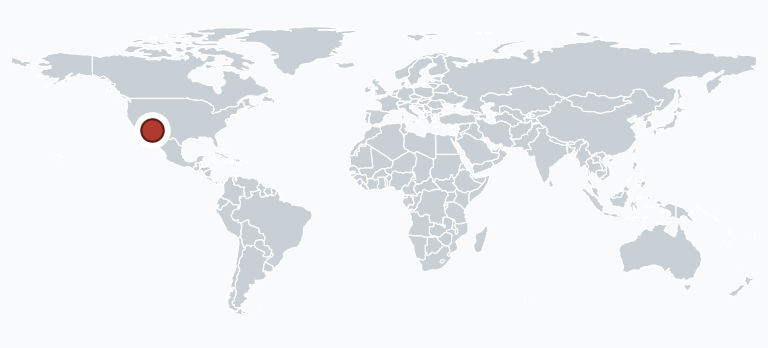
\includegraphics[width=\linewidth,keepaspectratio]{../figures/campus-locators/aifab-003-world-locator.png}
\par\smallskip
{\sffamily\scriptsize Coordinates: 33.775, -112.161.\par}
{\sffamily\scriptsize\color{black!68} Coordinates from the cited public map.\nobreak\textsuperscript{\href{\detokenize{https://maps.app.goo.gl/rgCqvY34HuN419jw8}}{\textcolor{accent}{1}}}\par}
\end{minipage}
\par\vspace{0.9em}
\noindent
\begin{minipage}[t]{\textwidth}
\raggedright
% Image-left evidence-right profile row
\begin{minipage}[t]{0.64\textwidth}
\vspace{0pt}\raggedright
\includegraphics[width=\linewidth,height=0.42\textheight,keepaspectratio,trim=0 0bp 0 0bp,clip]{../assets/campus-imagery/aifab-003.png}
\end{minipage}
\hfill
\begin{minipage}[t]{0.32\textwidth}
\vspace{0pt}\vspace{1.0em}\raggedright
{\sffamily\scriptsize Image: U.S. Department of Agriculture, National Agriculture Imagery Program (public domain); photographed June 16, 2023; source extract 1 m grid; 4 km view.\nobreak\textsuperscript{\href{\detokenize{https://planetarycomputer.microsoft.com/dataset/naip}}{\textcolor{accent}{9}}} Yellow cross: cited location point.\par}
\medskip
{\footnotesize TSMC identifies the Phoenix campus, where Fab 1 is in N4 high-volume production and additional fabs are being built for N3, N2, and A16.\nobreak\textsuperscript{\href{\detokenize{https://www.tsmc.com/static/abouttsmcaz/index.htm}}{\textcolor{accent}{2}},\href{\detokenize{https://investor.tsmc.com/chinese/encrypt/files/encrypt_file/reports/2026-04/3cef85204275f94fd111485cfdf4adb3c0263c45/TSMC}\%\detokenize{201Q26}\%\detokenize{20Transcript.pdf}}{\textcolor{accent}{3}}}\par}
\medskip
{\footnotesize\textbf{Documented wafer-fabrication capability:} Fab 1 is in N4 high-volume production; Fab 2's structure is complete with N3 high-volume production targeted for the second half of 2027; Fab 3 is under construction for N2/A16; Fab 4 and the first advanced-packaging fab are in initial construction.\nobreak\textsuperscript{\href{\detokenize{https://www.tsmc.com/static/abouttsmcaz/index.htm}}{\textcolor{accent}{2}},\href{\detokenize{https://investor.tsmc.com/chinese/encrypt/files/encrypt_file/reports/2026-04/3cef85204275f94fd111485cfdf4adb3c0263c45/TSMC}\%\detokenize{201Q26}\%\detokenize{20Transcript.pdf}}{\textcolor{accent}{3}}}\par}
\end{minipage}
\end{minipage}
\par\vspace{0.65em}
\medskip
{\footnotesize\textbf{Named data-center AI accelerators or programs:}\par}
\begin{itemize}[leftmargin=1.25em,itemsep=0.35em,topsep=0.15em,parsep=0pt]
\item {\footnotesize\textbf{NVIDIA --- Blackwell.} NVIDIA states that TSMC is producing Blackwell chips at its Arizona campus.\nobreak\textsuperscript{\href{\detokenize{https://www.tsmc.com/static/abouttsmcaz/index.htm}}{\textcolor{accent}{2}},\href{\detokenize{https://blogs.nvidia.com/blog/tsmc-blackwell-manufacturing/}}{\textcolor{accent}{4}},\href{\detokenize{https://developer.nvidia.com/blog/nvidia-blackwell-platform-sets-new-llm-inference-records-in-mlperf-inference-v4-1/}}{\textcolor{accent}{5}}}\par {\scriptsize\color{black!62}\textbf{Limits of the evidence:} The source confirms some Blackwell production in Arizona but does not state what share is made there or whether every Blackwell version is included.\par}}
\item {\footnotesize\textbf{Tesla --- AI5.} In July 2025, Tesla's CEO said TSMC would make AI5 first in Taiwan and then in Arizona.\nobreak\textsuperscript{\href{\detokenize{https://www.tsmc.com/static/abouttsmcaz/index.htm}}{\textcolor{accent}{2}},\href{\detokenize{https://www.kedglobal.com/korean-chipmakers/newsView/ked202507280001}}{\textcolor{accent}{6}},\href{\detokenize{https://www.cnbc.com/2025/10/22/elon-musk-tesla-ai5-nvidia.html}}{\textcolor{accent}{7}},\href{\detokenize{https://www.notateslaapp.com/news/3974/musk-says-teslas-ai5-chip-is-done-not-coming-to-vehicles-first}}{\textcolor{accent}{8}}}\par {\scriptsize\color{black!62}\textbf{Limits of the evidence:} A stated plan; the sources reviewed report no process, start date, share, or output for Arizona. Musk said in April 2026 that AI5 would first serve Optimus and Tesla's supercomputer clusters.\par}}
\end{itemize}
\smallskip
{\sffamily\scriptsize\color{black!62}\textbf{Other public catalogues (same campus; reviewed August 25, 2026):} \href{\detokenize{https://en.wikipedia.org/w/index.php?title=List_of_semiconductor_fabrication_plants&oldid=1370451124}\#\detokenize{Open_plants}}{Wikipedia fab list}; \href{\detokenize{https://www.wikidata.org/w/index.php?title=Q135913497&oldid=2485030743}}{Wikidata}; \href{\detokenize{https://github.com/aminalav/chip-sense/blob/93d22afe9e1309a7bebd6c7c96541f069f1d67ac/src/data/fab-sites.json}\#\detokenize{L13-L20}}{Chip Sense}.\par}
\medskip
{\sffamily\scriptsize\setlength{\emergencystretch}{1.5em}\textbf{Sources.} \textsuperscript{1}\,Google Maps. \href{\detokenize{https://maps.app.goo.gl/rgCqvY34HuN419jw8}}{\enquote{TSMC Arizona campus.}} Accessed August 11, 2026; \textsuperscript{2}\,TSMC. \href{\detokenize{https://www.tsmc.com/static/abouttsmcaz/index.htm}}{\enquote{TSMC Arizona corporate site and manufacturing overview.}} Accessed August 11, 2026; \textsuperscript{3}\,TSMC. \href{\detokenize{https://investor.tsmc.com/chinese/encrypt/files/encrypt_file/reports/2026-04/3cef85204275f94fd111485cfdf4adb3c0263c45/TSMC}\%\detokenize{201Q26}\%\detokenize{20Transcript.pdf}}{\enquote{First Quarter 2026 Earnings Conference Transcript.}} April 16, 2026; \textsuperscript{4}\,NVIDIA. \href{\detokenize{https://blogs.nvidia.com/blog/tsmc-blackwell-manufacturing/}}{\enquote{The Engines of American-Made Intelligence: NVIDIA and TSMC Celebrate First NVIDIA Blackwell Wafer Produced in the US.}} October 17, 2025; \textsuperscript{5}\,NVIDIA. \href{\detokenize{https://developer.nvidia.com/blog/nvidia-blackwell-platform-sets-new-llm-inference-records-in-mlperf-inference-v4-1/}}{\enquote{NVIDIA Blackwell Platform Sets New LLM Inference Records in MLPerf Inference v4.1.}} August 28, 2024; \textsuperscript{6}\,KED Global. \href{\detokenize{https://www.kedglobal.com/korean-chipmakers/newsView/ked202507280001}}{\enquote{Samsung clinches \$16.5 billion chipmaking deal from Tesla.}} July 28, 2025; \textsuperscript{7}\,CNBC. \href{\detokenize{https://www.cnbc.com/2025/10/22/elon-musk-tesla-ai5-nvidia.html}}{\enquote{Tesla `not about to replace Nvidia' as EV maker develops chips for cars, robots, Musk says.}} October 22, 2025; \textsuperscript{8}\,Not a Tesla App. \href{\detokenize{https://www.notateslaapp.com/news/3974/musk-says-teslas-ai5-chip-is-done-not-coming-to-vehicles-first}}{\enquote{Musk Says Tesla's AI5 Chip is Done, Not Coming to Cars First.}} April 15, 2026; \textsuperscript{9}\,U.S. Department of Agriculture. \href{\detokenize{https://planetarycomputer.microsoft.com/dataset/naip}}{\enquote{National Agriculture Imagery Program.}} Accessed August 23, 2026.\par}
\vfill
\noindent{\color{hairline}\rule{\linewidth}{0.4pt}}\par\smallskip
{\sffamily\scriptsize\color{black!58} Evidence reviewed through August 25, 2026.\par}
\end{minipage}
\clearpage
% Campus profile AIFAB-026
\markright{Dresden Fab 1 campus}
\noindent\begin{minipage}[t][0.90\textheight][t]{\textwidth}
\noindent\begin{minipage}[t]{0.69\textwidth}
\raggedright
{\sffamily\bfseries\Large\color{accent} Dresden Fab 1 campus\par}
\smallskip
{\sffamily\small\textbf{Operator:} GlobalFoundries\quad \textbf{Location:} Dresden, Saxony, DEU\par}
{\sffamily\footnotesize\color{black!68}\textbf{Facility status:} Operating; expansion under construction (as of 2026-08-25)\par}
\end{minipage}
\hfill
\begin{minipage}[t]{0.27\textwidth}
\raggedright
{\sffamily\bfseries\footnotesize World location}\par\smallskip
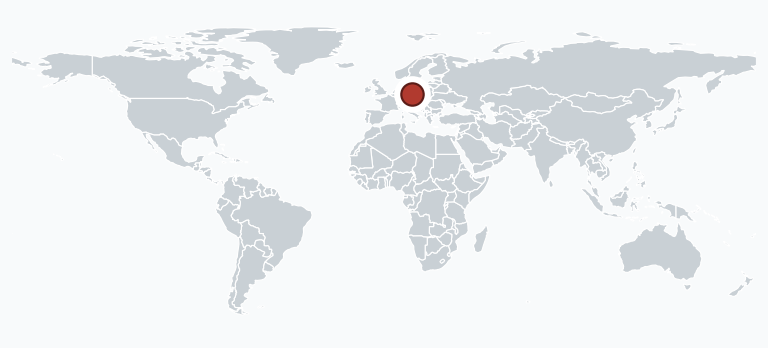
\includegraphics[width=\linewidth,keepaspectratio]{../figures/campus-locators/aifab-026-world-locator.png}
\par\smallskip
{\sffamily\scriptsize Coordinates: 51.126, 13.717.\par}
{\sffamily\scriptsize\color{black!68} Coordinates are the representative point returned for the cited OpenStreetMap feature.\nobreak\textsuperscript{\href{\detokenize{https://www.openstreetmap.org/way/10818500}}{\textcolor{accent}{1}}}\par}
\end{minipage}
\par\vspace{0.9em}
\noindent
\begin{minipage}[t]{\textwidth}
\raggedright
% Image-left evidence-right profile row
\begin{minipage}[t]{0.64\textwidth}
\vspace{0pt}\raggedright
\includegraphics[width=\linewidth,height=0.42\textheight,keepaspectratio,trim=0 0bp 0 0bp,clip]{../assets/campus-imagery/aifab-026.png}
\end{minipage}
\hfill
\begin{minipage}[t]{0.32\textwidth}
\vspace{0pt}\vspace{1.0em}\raggedright
{\sffamily\scriptsize Source: GeoSN, dl-de/by-2-0 (www.govdata.de/dl-de/by-2-0); SN DOP 020 RGB; photographed March 19 and April 7, 2024; source extract 0.976562 m grid; 4 km view; cropped and annotated by the authors.\nobreak\textsuperscript{\href{\detokenize{https://geomis.sachsen.de/geomis-client/?lang=de}\#\detokenize{/datasets/iso/1d088a9c-a3bb-4682-a3cb-10129e2f2be0}}{\textcolor{accent}{5}}} Yellow cross: cited location point.\par}
\medskip
{\footnotesize GlobalFoundries identifies Dresden as an operating high-volume manufacturing campus that makes 22FDX chips; an expansion is under construction.\nobreak\textsuperscript{\href{\detokenize{https://www.openstreetmap.org/way/10818500}}{\textcolor{accent}{1}},\href{\detokenize{https://investors.gf.com/static-files/ef3116da-5334-46e0-9b6c-56d3e67b1b92}}{\textcolor{accent}{2}},\href{\detokenize{https://gf.com/manufacturing/dresden/}}{\textcolor{accent}{3}},\href{\detokenize{https://gf.com/news-and-events/news/globalfoundries-and-nxp-to-deliver-next-generation-22fdx-solutions-for-automotive-iot-and-smart-mobile/}}{\textcolor{accent}{4}}}\par}
\medskip
{\footnotesize\textbf{Documented wafer-fabrication capability:} GlobalFoundries identifies Dresden as an operating high-volume manufacturing site and states that 22FDX chips are made there; the SPRINT expansion broke ground in 2026.\nobreak\textsuperscript{\href{\detokenize{https://investors.gf.com/static-files/ef3116da-5334-46e0-9b6c-56d3e67b1b92}}{\textcolor{accent}{2}},\href{\detokenize{https://gf.com/manufacturing/dresden/}}{\textcolor{accent}{3}},\href{\detokenize{https://gf.com/news-and-events/news/globalfoundries-and-nxp-to-deliver-next-generation-22fdx-solutions-for-automotive-iot-and-smart-mobile/}}{\textcolor{accent}{4}}}\par}
\end{minipage}
\end{minipage}
\par\vspace{0.65em}
\medskip
{\footnotesize\textbf{Named data-center AI accelerators or programs:} None identified in the sources reviewed.\par}
\smallskip
{\sffamily\scriptsize\color{black!62}\textbf{Other public catalogues (same campus; reviewed August 25, 2026):} \href{\detokenize{https://en.wikipedia.org/w/index.php?title=List_of_semiconductor_fabrication_plants&oldid=1370451124}\#\detokenize{Open_plants}}{Wikipedia fab list}; \href{\detokenize{https://www.wikidata.org/w/index.php?title=Q115408033&oldid=1820322161}}{Wikidata}; \href{\detokenize{https://github.com/aminalav/chip-sense/blob/93d22afe9e1309a7bebd6c7c96541f069f1d67ac/src/data/fab-sites.json}\#\detokenize{L233-L240}}{Chip Sense}.\par}
\medskip
{\sffamily\scriptsize\setlength{\emergencystretch}{1.5em}\textbf{Sources.} \textsuperscript{1}\,OpenStreetMap contributors. \href{\detokenize{https://www.openstreetmap.org/way/10818500}}{\enquote{GlobalFoundries Fab 1 mapped industrial site, OSM way 10818500.}} Accessed August 25, 2026; \textsuperscript{2}\,GlobalFoundries. \href{\detokenize{https://investors.gf.com/static-files/ef3116da-5334-46e0-9b6c-56d3e67b1b92}}{\enquote{2025 Form 20-F.}} February 27, 2026; \textsuperscript{3}\,GlobalFoundries. \href{\detokenize{https://gf.com/manufacturing/dresden/}}{\enquote{Dresden manufacturing site.}} Accessed August 25, 2026; \textsuperscript{4}\,GlobalFoundries and NXP. \href{\detokenize{https://gf.com/news-and-events/news/globalfoundries-and-nxp-to-deliver-next-generation-22fdx-solutions-for-automotive-iot-and-smart-mobile/}}{\enquote{GlobalFoundries and NXP to Deliver Next-Generation 22FDX Solutions for Automotive, IoT and Smart Mobile.}} October 23, 2024; \textsuperscript{5}\,Landesamt für Geobasisinformation Sachsen (GeoSN). \href{\detokenize{https://geomis.sachsen.de/geomis-client/?lang=de}\#\detokenize{/datasets/iso/1d088a9c-a3bb-4682-a3cb-10129e2f2be0}}{\enquote{SN DOP 020 RGB.}} Accessed August 23, 2026.\par}
\vfill
\noindent{\color{hairline}\rule{\linewidth}{0.4pt}}\par\smallskip
{\sffamily\scriptsize\color{black!58} Evidence reviewed through August 25, 2026.\par}
\end{minipage}
\clearpage
% Campus profile AIFAB-024
\markright{ESMC Dresden campus}
\noindent\begin{minipage}[t][0.90\textheight][t]{\textwidth}
\noindent\begin{minipage}[t]{0.69\textwidth}
\raggedright
{\sffamily\bfseries\Large\color{accent} ESMC Dresden campus\par}
\smallskip
{\sffamily\small\textbf{Operator:} ESMC / TSMC\quad \textbf{Location:} Dresden, Saxony, DEU\par}
{\sffamily\footnotesize\color{black!68}\textbf{Facility status:} Under construction (as of 2026-08-25)\par}
\end{minipage}
\hfill
\begin{minipage}[t]{0.27\textwidth}
\raggedright
{\sffamily\bfseries\footnotesize World location}\par\smallskip
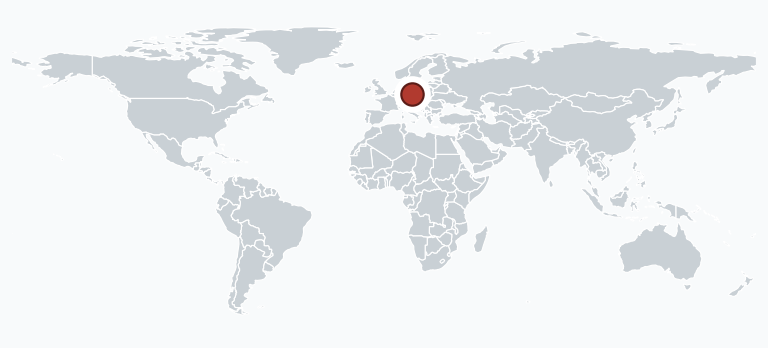
\includegraphics[width=\linewidth,keepaspectratio]{../figures/campus-locators/aifab-024-world-locator.png}
\par\smallskip
{\sffamily\scriptsize Coordinates: 51.130, 13.746.\par}
{\sffamily\scriptsize\color{black!68} Coordinates are the representative point returned for the cited OpenStreetMap feature.\nobreak\textsuperscript{\href{\detokenize{https://www.openstreetmap.org/way/583767292}}{\textcolor{accent}{1}}}\par}
\end{minipage}
\par\vspace{0.9em}
\noindent
\begin{minipage}[t]{\textwidth}
\raggedright
% Image-left evidence-right profile row
\begin{minipage}[t]{0.64\textwidth}
\vspace{0pt}\raggedright
\includegraphics[width=\linewidth,height=0.42\textheight,keepaspectratio,trim=0 0bp 0 0bp,clip]{../assets/campus-imagery/aifab-024.png}
\end{minipage}
\hfill
\begin{minipage}[t]{0.32\textwidth}
\vspace{0pt}\vspace{1.0em}\raggedright
{\sffamily\scriptsize Dresden Orthophotos 2025/2026 primary with GeoSN SN DOP 020 RGB no-data edge fill; source dated March 13, 2026; source extract 0.2 m grid; 2.2 km view. Datenquellen: Landeshauptstadt Dresden, dl-de/by-2-0 (www.govdata.de/dl-de/by-2-0), opendata.dresden.de, Orthophotos 2025/2026, March 13, 2026 where available; exact-white city-layer no-data edge areas filled with GeoSN SN DOP 020 RGB, dl-de/by-2-0, photographed March 19 and April 7, 2024; cropped, composited, and annotated by the authors.\nobreak\textsuperscript{\href{\detokenize{https://stadtplan.dresden.de/public/ogcsl.ashx?SERVICE=WMTS&REQUEST=GetCapabilities&VERSION=1.0.0&PKGID=4}}{\textcolor{accent}{4}}} Yellow cross: cited location point.\par}
\medskip
{\footnotesize TSMC and ESMC identify this separate campus as under construction and planned for 16/12 nm production, primarily for automotive and industrial customers.\nobreak\textsuperscript{\href{\detokenize{https://www.openstreetmap.org/way/583767292}}{\textcolor{accent}{1}},\href{\detokenize{https://pr.tsmc.com/english/news/3169}}{\textcolor{accent}{2}},\href{\detokenize{https://www.lds.sachsen.de/bekanntmachung/anlagen/ESMC_Bescheid_1._TG_geschw_LDS.pdf}}{\textcolor{accent}{3}}}\par}
\medskip
{\footnotesize\textbf{Documented wafer-fabrication capability:} Official plan for 40,000 300 mm wafers/month using 28/22 nm planar CMOS and 16/12 nm FinFET; official target markets are automotive and industrial.\nobreak\textsuperscript{\href{\detokenize{https://pr.tsmc.com/english/news/3169}}{\textcolor{accent}{2}},\href{\detokenize{https://www.lds.sachsen.de/bekanntmachung/anlagen/ESMC_Bescheid_1._TG_geschw_LDS.pdf}}{\textcolor{accent}{3}}}\par}
\end{minipage}
\end{minipage}
\par\vspace{0.65em}
\medskip
{\footnotesize\textbf{Named data-center AI accelerators or programs:} None identified in the sources reviewed.\par}
\medskip
{\sffamily\scriptsize\setlength{\emergencystretch}{1.5em}\textbf{Sources.} \textsuperscript{1}\,OpenStreetMap contributors. \href{\detokenize{https://www.openstreetmap.org/way/583767292}}{\enquote{ESMC mapped construction site, OSM way 583767292.}} Accessed August 11, 2026; \textsuperscript{2}\,TSMC / ESMC. \href{\detokenize{https://pr.tsmc.com/english/news/3169}}{\enquote{ESMC Breaks Ground on Dresden Fab.}} August 20, 2024; \textsuperscript{3}\,State Directorate of Saxony. \href{\detokenize{https://www.lds.sachsen.de/bekanntmachung/anlagen/ESMC_Bescheid_1._TG_geschw_LDS.pdf}}{\enquote{ESMC Dresden construction permit, first partial approval.}} 2025; \textsuperscript{4}\,Landeshauptstadt Dresden (primary); Landesamt für Geobasisinformation Sachsen / GeoSN (edge fill). \href{\detokenize{https://stadtplan.dresden.de/public/ogcsl.ashx?SERVICE=WMTS&REQUEST=GetCapabilities&VERSION=1.0.0&PKGID=4}}{\enquote{Dresden Orthophotos 2025/2026 primary with GeoSN SN DOP 020 RGB no-data edge fill.}} Accessed August 23, 2026.\par}
\vfill
\noindent{\color{hairline}\rule{\linewidth}{0.4pt}}\par\smallskip
{\sffamily\scriptsize\color{black!58} Evidence reviewed through August 25, 2026.\par}
\end{minipage}
\clearpage
% Campus profile AIFAB-015
\markright{Leixlip campus (Fab 24 / Fab 34)}
\noindent\begin{minipage}[t][0.90\textheight][t]{\textwidth}
\noindent\begin{minipage}[t]{0.69\textwidth}
\raggedright
{\sffamily\bfseries\Large\color{accent} Leixlip campus (Fab 24 / Fab 34)\par}
\smallskip
{\sffamily\small\textbf{Operator:} Intel\quad \textbf{Location:} Leixlip, Kildare, IRL\par}
{\sffamily\footnotesize\color{black!68}\textbf{Facility status:} Operating; expansion under construction (as of 2026-08-25)\par}
\end{minipage}
\hfill
\begin{minipage}[t]{0.27\textwidth}
\raggedright
{\sffamily\bfseries\footnotesize World location}\par\smallskip
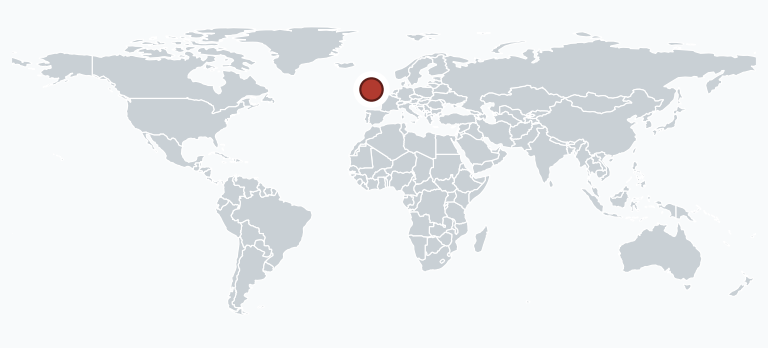
\includegraphics[width=\linewidth,keepaspectratio]{../figures/campus-locators/aifab-015-world-locator.png}
\par\smallskip
{\sffamily\scriptsize Coordinates: 53.375, -6.513.\par}
{\sffamily\scriptsize\color{black!68} Coordinates from the cited Irish EPA facility record.\nobreak\textsuperscript{\href{\detokenize{https://epawebapp.epa.ie/licences/lic_eDMS/090151b28063c199.pdf}}{\textcolor{accent}{1}}}\par}
\end{minipage}
\par\vspace{0.9em}
\noindent
\begin{minipage}[t]{\textwidth}
\raggedright
% Image-left evidence-right profile row
\begin{minipage}[t]{0.64\textwidth}
\vspace{0pt}\raggedright
\includegraphics[width=\linewidth,height=0.42\textheight,keepaspectratio,trim=0 0bp 0 0bp,clip]{../assets/campus-imagery/aifab-015.png}
\end{minipage}
\hfill
\begin{minipage}[t]{0.32\textwidth}
\vspace{0pt}\vspace{1.0em}\raggedright
{\sffamily\scriptsize World Imagery; source imagery dated September 4, 2023; source extract 0.585938 m grid; 2.4 km view. Source: Esri, Vantor, Earthstar Geographics, and the GIS User Community. Local imagery: Vantor Vivid Advanced (WV02), source dated 2023-09-04, Raster Basemaps 2025.R10. Map image is the intellectual property of Esri and is used herein under license. Copyright © 2026 Esri and its licensors. All rights reserved. Cropped and annotated by the authors.\nobreak\textsuperscript{\href{\detokenize{https://www.arcgis.com/home/item.html?id=10df2279f9684e4a9f6a7f08febac2a9}}{\textcolor{accent}{5}}} Yellow cross: cited location point.\par}
\medskip
{\footnotesize Intel identifies Fab 24 and Fab 34 on one Leixlip campus, with Intel 4 and Intel 3 high-volume manufacturing and a capacity expansion under way.\nobreak\textsuperscript{\href{\detokenize{https://www.intc.com/filings-reports/all-sec-filings/content/0000050863-26-000011/intc-20251227.htm}}{\textcolor{accent}{2}},\href{\detokenize{https://web.archive.org/web/20260814012648/https://newsroom.intel.com/intel-foundry/intel-invests-5-billion-euro-to-expand-manufacturing-in-europe}}{\textcolor{accent}{3}},\href{\detokenize{https://leap.epa.ie/docs/81d5494a-236b-437f-b142-5afa039042a4.pdf}}{\textcolor{accent}{4}}}\par}
\medskip
{\footnotesize\textbf{Documented wafer-fabrication capability:} Fab 34 performs Intel 4 and Intel 3 high-volume manufacturing; a EUR5 billion Intel 3 and Xeon capacity expansion is under way.\nobreak\textsuperscript{\href{\detokenize{https://www.intc.com/filings-reports/all-sec-filings/content/0000050863-26-000011/intc-20251227.htm}}{\textcolor{accent}{2}},\href{\detokenize{https://web.archive.org/web/20260814012648/https://newsroom.intel.com/intel-foundry/intel-invests-5-billion-euro-to-expand-manufacturing-in-europe}}{\textcolor{accent}{3}}}\par}
\end{minipage}
\end{minipage}
\par\vspace{0.65em}
\medskip
{\footnotesize\textbf{Named data-center AI accelerators or programs:} None identified in the sources reviewed.\par}
\smallskip
{\sffamily\scriptsize\color{black!62}\textbf{Other public catalogues (same campus; reviewed August 25, 2026):} \href{\detokenize{https://en.wikipedia.org/w/index.php?title=List_of_semiconductor_fabrication_plants&oldid=1370451124}\#\detokenize{Open_plants}}{Wikipedia fab list}; \href{\detokenize{https://www.wikidata.org/w/index.php?title=Q113324961&oldid=1694261236}}{Wikidata}; \href{\detokenize{https://github.com/aminalav/chip-sense/blob/93d22afe9e1309a7bebd6c7c96541f069f1d67ac/src/data/fab-sites.json}\#\detokenize{L153-L160}}{Chip Sense}.\par}
\medskip
{\sffamily\scriptsize\setlength{\emergencystretch}{1.5em}\textbf{Sources.} \textsuperscript{1}\,Intel Ireland Ltd. \href{\detokenize{https://epawebapp.epa.ie/licences/lic_eDMS/090151b28063c199.pdf}}{\enquote{Annual Environmental Report 2016.}} April 27, 2017; \textsuperscript{2}\,Intel. \href{\detokenize{https://www.intc.com/filings-reports/all-sec-filings/content/0000050863-26-000011/intc-20251227.htm}}{\enquote{Intel 2025 annual report on Form 10-K.}} 2026; \textsuperscript{3}\,Intel. \href{\detokenize{https://web.archive.org/web/20260814012648/https://newsroom.intel.com/intel-foundry/intel-invests-5-billion-euro-to-expand-manufacturing-in-europe}}{\enquote{Intel invests EUR5 billion to expand manufacturing in Europe.}} July 13, 2026; \textsuperscript{4}\,Intel Ireland Limited. \href{\detokenize{https://leap.epa.ie/docs/81d5494a-236b-437f-b142-5afa039042a4.pdf}}{\enquote{Annual Environmental Report (AER) 2025.}} April 28, 2026; \textsuperscript{5}\,Esri. \href{\detokenize{https://www.arcgis.com/home/item.html?id=10df2279f9684e4a9f6a7f08febac2a9}}{\enquote{World Imagery.}} Accessed August 23, 2026.\par}
\vfill
\noindent{\color{hairline}\rule{\linewidth}{0.4pt}}\par\smallskip
{\sffamily\scriptsize\color{black!58} Evidence reviewed through August 25, 2026.\par}
\end{minipage}
\clearpage
% Campus profile AIFAB-016
\markright{Kiryat Gat campus / Fab 28}
\noindent\begin{minipage}[t][0.90\textheight][t]{\textwidth}
\noindent\begin{minipage}[t]{0.69\textwidth}
\raggedright
{\sffamily\bfseries\Large\color{accent} Kiryat Gat campus / Fab 28\par}
\smallskip
{\sffamily\small\textbf{Operator:} Intel\quad \textbf{Location:} Kiryat Gat, Southern District, ISR\par}
{\sffamily\footnotesize\color{black!68}\textbf{Facility status:} Operating (as of 2026-08-25)\par}
\end{minipage}
\hfill
\begin{minipage}[t]{0.27\textwidth}
\raggedright
{\sffamily\bfseries\footnotesize World location}\par\smallskip
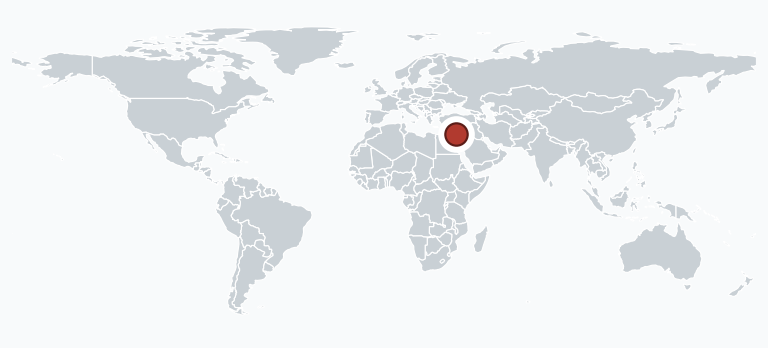
\includegraphics[width=\linewidth,keepaspectratio]{../figures/campus-locators/aifab-016-world-locator.png}
\par\smallskip
{\sffamily\scriptsize Coordinates: 31.594, 34.789.\par}
{\sffamily\scriptsize\color{black!68} Coordinates from the cited Israeli government facility record.\nobreak\textsuperscript{\href{\detokenize{https://www.gov.il/apps/sviva/airq/atar_svivati_emission_details?atarsvivati=172589&layer=divuchim2020}}{\textcolor{accent}{1}}}\par}
\end{minipage}
\par\vspace{0.9em}
\noindent
\begin{minipage}[t]{\textwidth}
\raggedright
% Image-left evidence-right profile row
\begin{minipage}[t]{0.64\textwidth}
\vspace{0pt}\raggedright
\includegraphics[width=\linewidth,height=0.42\textheight,keepaspectratio,trim=0 0bp 0 0bp,clip]{../assets/campus-imagery/aifab-016.png}
\end{minipage}
\hfill
\begin{minipage}[t]{0.32\textwidth}
\vspace{0pt}\vspace{1.0em}\raggedright
{\sffamily\scriptsize World Imagery; source imagery dates November 7, 2024 and December 24, 2024; source extract 0.830078 m grid; 3.4 km view. Source: Esri, Vantor, Earthstar Geographics, and the GIS User Community. Local imagery: Vantor Vivid (LG02), source dated 2024-11-07, Raster Basemaps 2026.R01; Vantor Vivid (LG01), source dated 2024-12-24, Raster Basemaps 2026.R01. Map image is the intellectual property of Esri and is used herein under license. Copyright © 2026 Esri and its licensors. All rights reserved. Cropped and annotated by the authors.\nobreak\textsuperscript{\href{\detokenize{https://www.arcgis.com/home/item.html?id=10df2279f9684e4a9f6a7f08febac2a9}}{\textcolor{accent}{5}}} Yellow cross: cited location point.\par}
\medskip
{\footnotesize Intel identifies Fab 28 as the operating Intel 7 facility at Kiryat Gat. Intel lists its Israel expansion as delayed or cancelled; that Kiryat Gat expansion, reported as Fab 38 and paused since mid-2024, is not counted separately.\nobreak\textsuperscript{\href{\detokenize{https://www.intc.com/filings-reports/all-sec-filings/content/0000050863-26-000011/intc-20251227.htm}}{\textcolor{accent}{2}},\href{\detokenize{https://web.archive.org/web/20260508212537/https://www.intel.com/content/www/us/en/corporate-responsibility/intel-in-israel.html}}{\textcolor{accent}{3}},\href{\detokenize{https://www.tomshardware.com/tech-industry/semiconductors/intels-fab-roadmap-examined}}{\textcolor{accent}{4}}}\par}
\medskip
{\footnotesize\textbf{Documented wafer-fabrication capability:} Intel 7\nobreak\textsuperscript{\href{\detokenize{https://www.intc.com/filings-reports/all-sec-filings/content/0000050863-26-000011/intc-20251227.htm}}{\textcolor{accent}{2}}}\par}
\end{minipage}
\end{minipage}
\par\vspace{0.65em}
\medskip
{\footnotesize\textbf{Named data-center AI accelerators or programs:} None identified in the sources reviewed.\par}
\smallskip
{\sffamily\scriptsize\color{black!62}\textbf{Other public catalogues (same campus; reviewed August 25, 2026):} \href{\detokenize{https://en.wikipedia.org/w/index.php?title=List_of_semiconductor_fabrication_plants&oldid=1370451124}\#\detokenize{Open_plants}}{Wikipedia fab list}; \href{\detokenize{https://www.wikidata.org/w/index.php?title=Q113325038&oldid=1694261910}}{Wikidata}; \href{\detokenize{https://github.com/aminalav/chip-sense/blob/93d22afe9e1309a7bebd6c7c96541f069f1d67ac/src/data/fab-sites.json}\#\detokenize{L163-L170}}{Chip Sense}.\par}
\medskip
{\sffamily\scriptsize\setlength{\emergencystretch}{1.5em}\textbf{Sources.} \textsuperscript{1}\,Israel Ministry of Environmental Protection. \href{\detokenize{https://www.gov.il/apps/sviva/airq/atar_svivati_emission_details?atarsvivati=172589&layer=divuchim2020}}{\enquote{PRTR facility record 172589: Intel Electronics Ltd. (Intel Kiryat Gat).}} Accessed August 11, 2026; \textsuperscript{2}\,Intel. \href{\detokenize{https://www.intc.com/filings-reports/all-sec-filings/content/0000050863-26-000011/intc-20251227.htm}}{\enquote{Intel 2025 annual report on Form 10-K.}} 2026; \textsuperscript{3}\,Intel. \href{\detokenize{https://web.archive.org/web/20260508212537/https://www.intel.com/content/www/us/en/corporate-responsibility/intel-in-israel.html}}{\enquote{Intel in Israel.}} Archived May 8, 2026; \textsuperscript{4}\,Tom's Hardware. \href{\detokenize{https://www.tomshardware.com/tech-industry/semiconductors/intels-fab-roadmap-examined}}{\enquote{Intel's fab roadmap examined --- Arizona, Ohio, Ireland, and the two deadlines deciding 14A process node.}} June 17, 2026; \textsuperscript{5}\,Esri. \href{\detokenize{https://www.arcgis.com/home/item.html?id=10df2279f9684e4a9f6a7f08febac2a9}}{\enquote{World Imagery.}} Accessed August 23, 2026.\par}
\vfill
\noindent{\color{hairline}\rule{\linewidth}{0.4pt}}\par\smallskip
{\sffamily\scriptsize\color{black!58} Evidence reviewed through August 25, 2026.\par}
\end{minipage}
\clearpage
% Campus profile AIFAB-033
\markright{Dholera semiconductor fab campus}
\noindent\begin{minipage}[t][0.90\textheight][t]{\textwidth}
\noindent\begin{minipage}[t]{0.69\textwidth}
\raggedright
{\sffamily\bfseries\Large\color{accent} Dholera semiconductor fab campus\par}
\smallskip
{\sffamily\small\textbf{Operator:} Tata Electronics\quad \textbf{Location:} Dholera, Gujarat, IND\par}
{\sffamily\footnotesize\color{black!68}\textbf{Facility status:} Under construction (as of 2026-08-25)\par}
\end{minipage}
\hfill
\begin{minipage}[t]{0.27\textwidth}
\raggedright
{\sffamily\bfseries\footnotesize World location}\par\smallskip
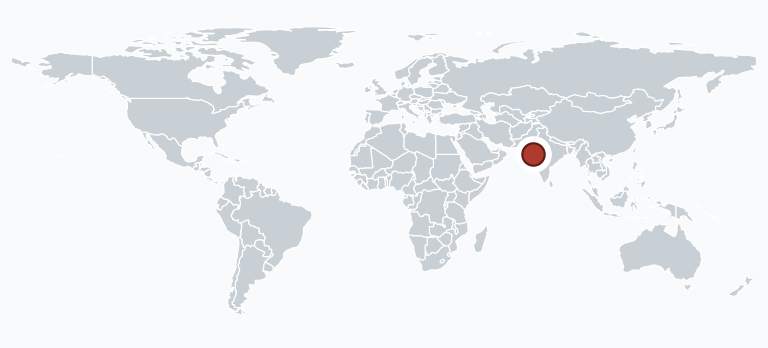
\includegraphics[width=\linewidth,keepaspectratio]{../figures/campus-locators/aifab-033-world-locator.png}
\par\smallskip
{\sffamily\scriptsize Coordinates: 22.226, 72.194.\par}
{\sffamily\scriptsize\color{black!68} Coordinates computed from the project polygon in the cited government record.\nobreak\textsuperscript{\href{\detokenize{https://environmentclearance.nic.in/writereaddata/FormB/agenda/0801202511837869SEACMinutesofthe982ndVC.pdf}}{\textcolor{accent}{1}}}\par}
\end{minipage}
\par\vspace{0.9em}
\noindent
\begin{minipage}[t]{\textwidth}
\raggedright
% Image-left evidence-right profile row
\begin{minipage}[t]{0.64\textwidth}
\vspace{0pt}\raggedright
\includegraphics[width=\linewidth,height=0.42\textheight,keepaspectratio,trim=0 0bp 0 0bp,clip]{../assets/campus-imagery/aifab-033.png}
\end{minipage}
\hfill
\begin{minipage}[t]{0.32\textwidth}
\vspace{0pt}\vspace{1.0em}\raggedright
{\sffamily\scriptsize World Imagery; source imagery dated March 7, 2026; source extract 0.585938 m grid; 2.4 km view. Source: Esri, Vantor, Earthstar Geographics, and the GIS User Community. Local imagery: Vantor Vivid (LG01), source dated 2026-03-07, Raster Basemaps 2026.R07. Map image is the intellectual property of Esri and is used herein under license. Copyright © 2026 Esri and its licensors. All rights reserved. Cropped and annotated by the authors.\nobreak\textsuperscript{\href{\detokenize{https://www.arcgis.com/home/item.html?id=10df2279f9684e4a9f6a7f08febac2a9}}{\textcolor{accent}{6}}} Yellow cross: cited location point.\par}
\medskip
{\footnotesize Official Tata sources identify the fab as under construction and name high-performance computing and AI among its intended markets. It is included because of that stated market focus, even though its most advanced planned process is 28 nm.\nobreak\textsuperscript{\href{\detokenize{https://environmentclearance.nic.in/writereaddata/FormB/agenda/0801202511837869SEACMinutesofthe982ndVC.pdf}}{\textcolor{accent}{1}},\href{\detokenize{https://www.tata.com/newsroom/business/first-indian-fab-semiconductor-dholera}}{\textcolor{accent}{2}},\href{\detokenize{https://www.tata.com/newsroom/business/tata-electronics-asml-semiconductor-ecosystem}}{\textcolor{accent}{3}},\href{\detokenize{https://sezindia.gov.in/node/2838}}{\textcolor{accent}{4}},\href{\detokenize{https://www.tata.com/content/dam/tata/pdf/fy25/Tata-Sons-Annual-Report-FY25.pdf}}{\textcolor{accent}{5}}}\par}
\medskip
{\footnotesize\textbf{Documented wafer-fabrication capability:} Planned 300 mm fab with a 28/40/55/90/110 nm portfolio; 50,000 wafers/month is the planned ultimate maximum, while an environmental-clearance record lists 32,000 IC wafers/month\nobreak\textsuperscript{\href{\detokenize{https://environmentclearance.nic.in/writereaddata/FormB/agenda/0801202511837869SEACMinutesofthe982ndVC.pdf}}{\textcolor{accent}{1}},\href{\detokenize{https://www.tata.com/newsroom/business/first-indian-fab-semiconductor-dholera}}{\textcolor{accent}{2}},\href{\detokenize{https://www.tata.com/newsroom/business/tata-electronics-asml-semiconductor-ecosystem}}{\textcolor{accent}{3}}}\par}
\end{minipage}
\end{minipage}
\par\vspace{0.65em}
\medskip
{\footnotesize\textbf{Named data-center AI accelerators or programs:} None identified in the sources reviewed.\par}
\smallskip
{\sffamily\scriptsize\color{black!62}\textbf{Other public catalogues (same campus; reviewed August 25, 2026):} \href{\detokenize{https://github.com/pranaykotas/india-semiconductor-tracker/blob/4d36dae28b2f25c2ffc8236ca1246142a79ce324/data/facilities.yml}\#\detokenize{L63-L77}}{India Semiconductor Tracker}.\par}
\medskip
{\sffamily\scriptsize\setlength{\emergencystretch}{1.5em}\textbf{Sources.} \textsuperscript{1}\,State Level Expert Appraisal Committee, Gujarat. \href{\detokenize{https://environmentclearance.nic.in/writereaddata/FormB/agenda/0801202511837869SEACMinutesofthe982ndVC.pdf}}{\enquote{Minutes of the 981st meeting of the State Level Expert Appraisal Committee.}} November 26, 2024; \textsuperscript{2}\,Tata Group. \href{\detokenize{https://www.tata.com/newsroom/business/first-indian-fab-semiconductor-dholera}}{\enquote{Tata Group to Build the Nation's First Fab in Dholera.}} February 29, 2024; \textsuperscript{3}\,Tata Group. \href{\detokenize{https://www.tata.com/newsroom/business/tata-electronics-asml-semiconductor-ecosystem}}{\enquote{Tata Electronics and ASML Announce Strategic Partnership.}} May 17, 2026; \textsuperscript{4}\,Government of India, Department of Commerce. \href{\detokenize{https://sezindia.gov.in/node/2838}}{\enquote{Notification of M/s. Tata Semiconductor Manufacturing Private Limited.}} April 9, 2026; \textsuperscript{5}\,Tata Sons Private Limited. \href{\detokenize{https://www.tata.com/content/dam/tata/pdf/fy25/Tata-Sons-Annual-Report-FY25.pdf}}{\enquote{Annual Report 2024-25.}} 2025; \textsuperscript{6}\,Esri. \href{\detokenize{https://www.arcgis.com/home/item.html?id=10df2279f9684e4a9f6a7f08febac2a9}}{\enquote{World Imagery.}} Accessed August 23, 2026.\par}
\vfill
\noindent{\color{hairline}\rule{\linewidth}{0.4pt}}\par\smallskip
{\sffamily\scriptsize\color{black!58} Evidence reviewed through August 25, 2026.\par}
\end{minipage}
\clearpage
